\chapter{Instantiating a cognitive model for predicting vehicle behavior}
\label{chap:behav_pred}

%\todo[inline]{check behavior prediction chapter for consistency}

Predicting future behavior and positions of other traffic participants from observations is a key problem, that needs to be solved by human drivers and automated vehicles alike to safely navigate their environment and to reach their desired goal.
Therefore, we picked behavior prediction as another task for investigating the potential of vector representations in automotive context.
In contrast to the task of classifying the current driving context presented in chapter~\ref{chap:driving_context_classification}, predicting future positions of vehicles is a regression problem, i.e., we are predicting continuous values such as spatial positions instead of discrete class labels.
However, future positions of vehicles not only depend on each vehicle's own past positions and dynamic data such as velocity and acceleration but also on the behavior of the other traffic participants in the vehicle's surroundings.
For instance, in a situation as shown in Fig.~\ref{fig:on_board_data_example}, the behavior of the target vehicle, as depicted by a solid blue and dotted orange line for past and future positions respectively, is influenced by the surrounding vehicles, as illustrated by solid and dotted gray lines for past and future positions respectively.
The target vehicle is approached from behind by a faster vehicle causing it to eventually change its lane to the right, which, for now, is still occupied by the ego-vehicle and another vehicle.
All of these external influences have an impact on the target vehicle's motion (and vice versa).
We hypothesize that structured vector representations will be able to capture these relations and mutual influence between traffic participants, which is necessary for reliable predictions.
As we aim for a model-free data representation, we avoid introducing any physical constraints or restrictions regarding our data-representation or the predicting models.
Although this allows for physically unrealistic or even impossible trajectory predictions, we want our neural network models to figure out the best predictions on their own without biasing them in any direction.
In this section, we present a representation of spatial information for multiple objects in semantic vectors of fixed length using the convolutive power introduced in Definition~\ref{def:conv_power}.
In contrast to other representations of spatial data, the dimensionality of our vectors is independent of the number of encoded entities.
We use this representation as input for simple feed-forward neural networks and more sophisticated \ac{LSTM}-based models and compare them against each other and a linear prediction model as the simplest baseline.
We conduct a thorough and detailed analysis and evaluate our  models on two different data sets, namely one proprietary data set recorded with an automated vehicle prototype and one publicly available trajectory data set.

We analyze our models with respect to the context, i.e., which model performs best depending on the current driving situation.
Furthermore, we investigate the influence of the composition of the training data on the models' performance.
Additionally, we show that by using our vector representation with a simple network architecture we can achieve results comparable to more complex models.

\section{Data and preprocessing}
\label{sec:data_preproc}

In this chapter, we use two different data sets for training and evaluation of our behavior prediction models, which we describe in more detail in subsequent sections.
We refer to those data sets as \emph{On-board} or $D_1$ (see section~\ref{subsec:onboard-dataset}), which is our main data set, and \emph{\acs{NGSIM}} or $D_2$ (see section~\ref{subsec:ngsim-dataset}), which is a publicly available data set used for reference and comparability.
In this section, we describe both data sets regarding available features, available sources of information as well as their key differences and the preprocessing procedure.

\subsection{On-board-sensors data set}
\label{subsec:onboard-dataset}

\begin{figure}[t!]
	\centering
	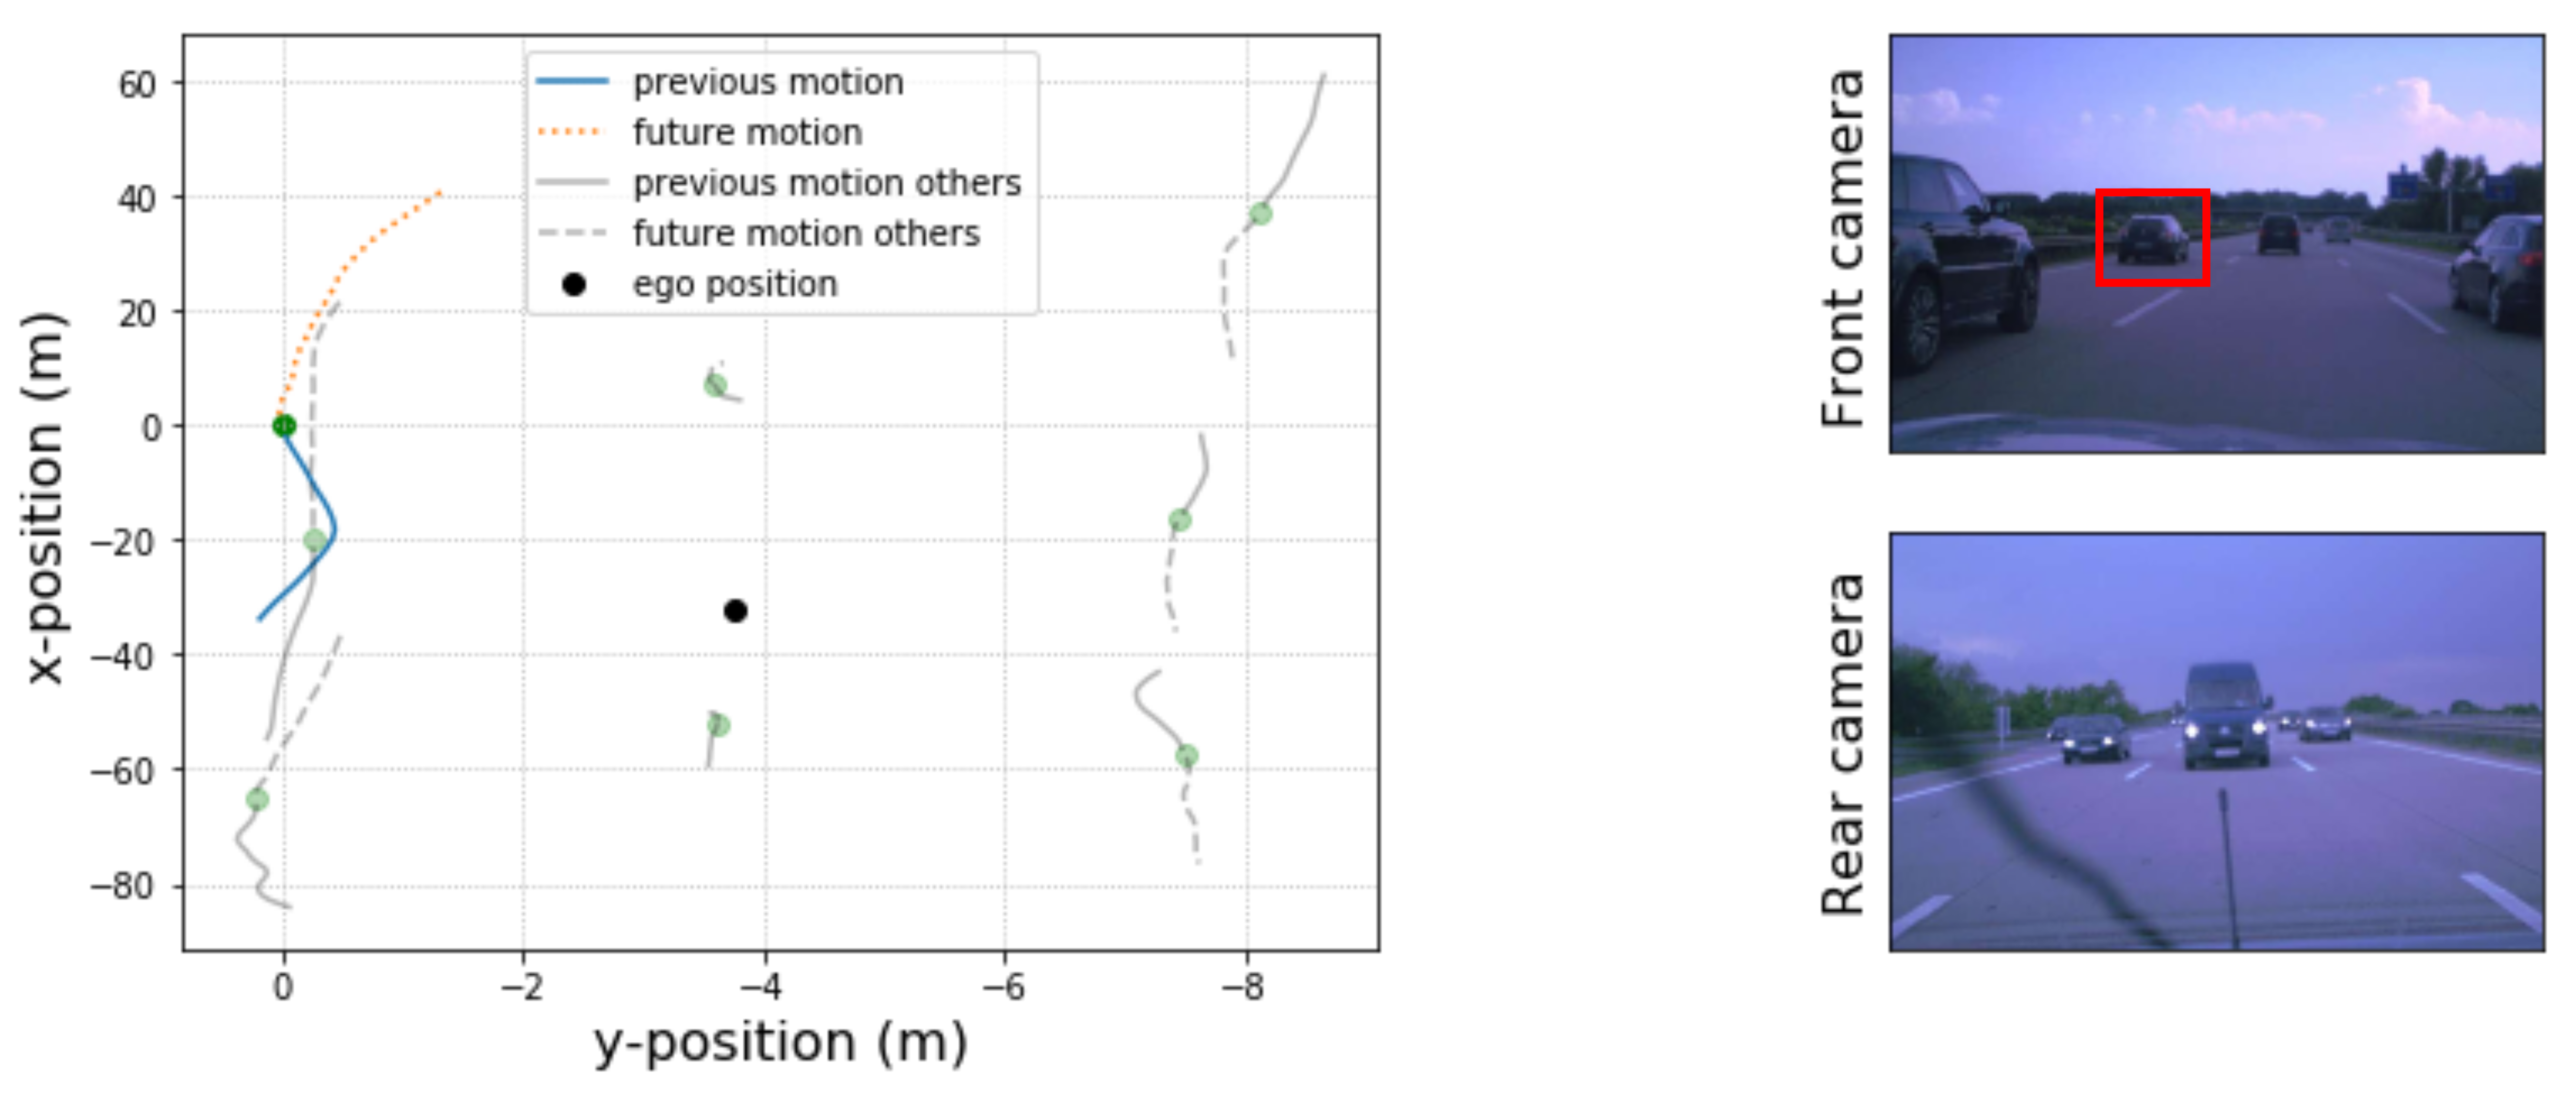
\includegraphics[width=\textwidth]{imgs/on_board_example_with_imgs_target.png}
    \caption{Data visualization of one driving situation example from the \emph{On-board} data set $D_1$.
        The dots in the left plot indicate the position of the vehicles and color-code the vehicle type (red=motorcycle, green=car, blue=truck, black=ego-vehicle), blue and orange lines show past and future motion of the target vehicle whereas gray lines depict the other vehicles' motion.
        The right figures show raw images of the ego-vehicle's front and rear camera with the target vehicle
    highlighted by a red rectangle.}\label{fig:on_board_data_example}
\end{figure}

This is our main data set used in this chapter.
It contains real-world data gathered using the on-board sensors of an automated vehicle prototype, which we refer to as the \emph{ego-vehicle}, during test drives mainly on highways in the area of Munich, Germany.
Therefore, we refer to this data set as the \emph{On-board} data set.
The data set contains object-lists with a variety of features obtained by fusing different sensor sources.
Apart from features about motion and behavior of the dynamic objects in the scene such as position, velocity and acceleration, which are estimated from \ac{LIDAR} sensors, there is also visual information like object type probabilities or lane information, which is acquired from additional camera sensors \parencite[see][for further information on the sensor setup]{Aeberhard2015}.
Table~\ref{tab:target_data_features} gives an overview and detailed description of the data features available in this data set, which are relevant for our models.
\begin{center}
	\begin{tabular}{|l | p{12cm}|}
		\hline
		\textbf{Data label} & \textbf{Description}\\ \hline
		Position & Lateral/Longitudinal position absolute/relative to the ego-vehicle's position estimated from range sensor readings \\ \hline
		Velocity& Lateral/Longitudinal velocity absolute/relative to the ego-vehicle's velocity estimated from range sensor readings \\ \hline
		Acceleration & Lateral/Lateral acceleration absolute/relative to the ego-vehicle's velocity estimated from range sensor readings \\ \hline
		Lane & Information about the lane relative to the ego-vehicle estimated from fused sensor reading (camera and range sensors) \\ \hline
		LaneBorderDistance & Distance to left/right border of the current lane estimated from fused sensor reading (camera and range sensors) \\ \hline
		LaneCurvature & Information about the lane curvature estimated from fused sensor reading (camera and range sensors) \\ \hline
		TypeProbability & Probability for the object being a of certain type (e.g. car or truck) estimated from camera sensors \\ \hline
	\end{tabular}
	\captionof{table}{Table depicting different features for dynamic objects within the training data}
	\label{tab:target_data_features}
\end{center}
In contrast to the data set used in chapter~\ref{chap:driving_context_classification}, the object-lists of the data set used here contain already preprocessed information as a fusion from the different available sensor sources.
This fused information about objects is available at a frequency of roughly \SI{5}{\hertz}.
The main feature of this data set is that all information (position, velocity, etc.) about vehicles other than the ego-vehicle is measured with respect to that ego-vehicle and its coordinate system.
Figure~\ref{fig:on_board_data_example} shows one example situation from this data set: the left plot depicts the already preprocessed) positional information of all vehicles detected by the ego-vehicle's on-board sensors.
The dots indicate the current position of the vehicles and color-code the vehicle type (red=motorcycle, green=car, blue=truck, black=ego-vehicle).
The blue and orange lines illustrate \SI{5}{\second} of past and future motion of the target vehicle respectively.
Solid and dashed gray lines depict the other vehicles' past and future motion respectively.
On the right-hand side, the raw images from the front and rear camera give an impression of the driving situation at hand with the target vehicle highlighted by a red box.
In total, the \emph{On-board} data set contains \num{3891} vehicles, which yield a total length of roughly \SI{28.3}{\hour} when adding up the time each individual vehicle is visible.

\subsection{\acs{NGSIM} US-101 data set}
\label{subsec:ngsim-dataset}

\begin{figure}[t!]
	\centering
	\resizebox{.95\textwidth}{!}{%
		\subfloat[\label{subfig:ngsim_highway_top_view}]{%
			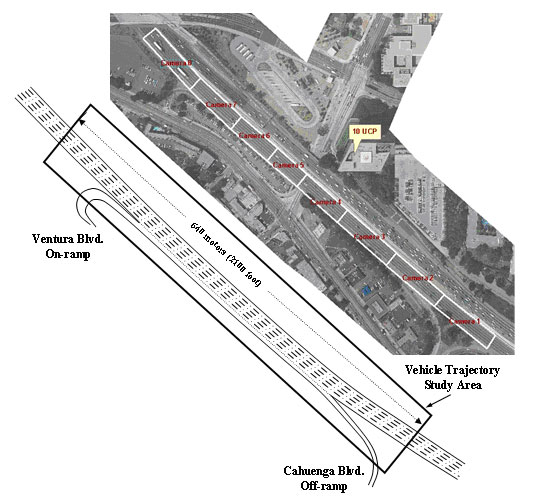
\includegraphics[height=4cm]{imgs/ngsim_highway_top_view.jpg}
		}
		\subfloat[\label{subfig:ngsim_example_xy}]{%
			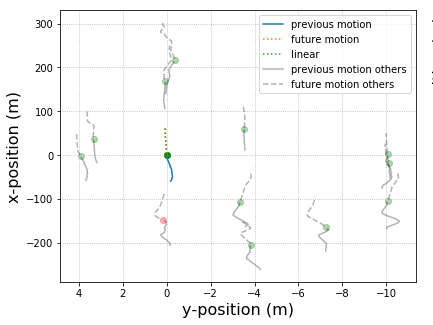
\includegraphics[height=4cm]{imgs/ngsim_example_xy.eps}
		}
	}
    \caption{Visualization of \emph{\ac{NGSIM}} data set:~\protect\subref{subfig:ngsim_highway_top_view} depicts the highway segment from top view perspective indicating the camera's position. Image source: \textcite{NGSIM-US101}.~\protect\subref{subfig:ngsim_example_xy} visualizes the data of one particular driving situation from the data set.}\label{fig:ngsim_dataset}
\end{figure}

The \ac{NGSIM} US-101 data set \parencite{NGSIM-US101} is a publicly available data set recorded on a segment of approximately \SI{640}{\meter} length with \num{6} lanes on the US-101 freeway in Los Angeles, California.
Although the data set was originally intended for driver behavior analysis and traffic flow models \parencite{He2017}, it has also been used to train trajectory prediction models, for instance proposed by \textcite{Altche2018, Deo2018}.
The data set was recorded using cameras observing freeway traffic from rooftops with trajectory-data being extracted later from the obtained video footage.
Figure~\ref{fig:ngsim_dataset} shows the recorded highway segment from top view perspective indicating the camera's position (Fig.~\ref{subfig:ngsim_highway_top_view}) as well as the visualization of one example driving situation (Fig.~\ref{subfig:ngsim_example_xy}).
The data set contains a total of \SI{45}{\minute} of driving data split into three \SI{15}{\minute} segments of mild, moderate and congesting traffic conditions.
Apart from positional information in lateral and longitudinal direction (in a global and local coordinate system), additional features such as instantaneous velocity, acceleration, vehicle size as well as the current lane are available for each vehicle.
The trajectory data is sampled with a frequency of \SI{10}{\hertz}.
The main difference to the \emph{On-board} data set is the fact that the \emph{\ac{NGSIM}} data set is recorded with external stationary cameras instead of a driving vehicle's on-board sensors.
Thus, there is no ego-vehicle present in the data and all information is available in absolute coordinates instead of being measured relative to one particular ego-vehicle.
In total, the \emph{\ac{NGSIM}} data set contains \num{5930} vehicles and therefore a total time of roughly \SI{91.3}{\hour} when adding up the time each individual vehicle is visible.

\subsection{Preprocessing}
\label{subsec:preproc}

In this section, we describe the preprocessing steps performed before training our models to prepare the trajectory information contained in our two data sets as input for neural networks.
Although we aim to keep these preprocessing steps as consistent as possible across both data sets, there are some mild differences, which we will point out here.
We aim to anticipate positions of dynamic objects \SI{5}{\second} into the future based on past positions \SI{5}{\second} prior to their current location for one object at a time.
As the two data sets are sampled at different frequencies, we interpolate the available data over \num{20} equidistant steps to achieve intervals of \SI{0.25}{\second} to improve consistency and comparability.
Furthermore, we translate the current position of the target vehicle, i.e., the vehicle to be predicted, to be the origin of the reference coordinate system.
That is, the current position of the target vehicle will be at position $\left(0,0\right)$ for all data samples consistently across both data sets (see Fig.~\ref{fig:on_board_data_example} and~\ref{subfig:ngsim_example_xy}).
The reason for this design choice is two-fold: on the one hand, we make samples from both data sets, which originally have different coordinate frames (global vs.\ ego-vehicle) as reference, more comparable and consistent.
On the other hand, by moving the current position of the target vehicle to the origin of the reference coordinate system of the sample, we prevent our models from treating similar trajectories differently due to positional variations.
Finally, to improve suitability of the data as input for neural networks, we divide all $x$-positions by a factor of \num{10} such that $x$-/$y$-values are scaled to a similar order of magnitude.
Since the \emph{\acs{NGSIM}} data set $D_2$ is sampled at a high frequency of \SI{10}{\hertz} and contains more data than the \emph{On-board} data set, we use only every \num{10}th data point.
Thereby, we avoid the creation of too many overlapping, and therefore too similar, data samples for the \emph{\ac{NGSIM}} data set.
Furthermore, we swapped the dimensions of the positions in the \emph{\ac{NGSIM}} data set such that for both data sets $x$- and $y$-direction correspond to longitudinal and lateral positions respectively.
For training and evaluating our models, we split both data sets into two distincts subset containing training $T_i \subset D_i$ and validation data $V_i \subset D_i$.
Those training and validation subsets contain \SI{90}{\percent} and \SI{10}{\percent} of the objects within the data sets respectively with $T_i \cap V_i = \varnothing$ to avoid testing our models on vehicles they have been trained with.

\subsection{Data set peculiarities}%
\label{subsec:data_set_peculiarities}

\begin{figure}[t]
    \centering
    \includegraphics[width=0.9\linewidth]{imgs/on_board_lane_change_example_with_imgs.png}
    \caption{Data visualization of one data sample from the \emph{On-board} data set $D_1$ containing a future lane change of the target vehicle.
        The dots in the left plot indicate the position of the vehicles and color-code the vehicle type (red=motorcycle, green=car, blue=truck, black=ego-vehicle), blue and orange lines show past and future motion of the target vehicle whereas gray lines depict the other vehicles' motion.
        The images in the top row show raw images recorded using the ego-vehicle's front and rear camera with the target vehicle highlighted by a red bounding box.}
    \label{fig:on_board_lane_change_example_with_imgs}
\end{figure}

In this section, we analyze the composition of our data sets regarding the amount of \enquote{interesting} behavior of the target vehicle.
Both, the \emph{On-board} and \emph{\ac{NGSIM}} data set consist of mainly highway driving, where we would expect mainly straight driving with the most interesting situations being the target vehicle, i.e., the vehicle whose motion we aim to predict, performing a lane change.
Hence, we are interested in the amount of situations where the target vehicle actually performs a lane change and how much more prominent normal straight driving is in both our data sets.
For the \emph{On-board} data set, we have information about the current lane as well as the distance to the lane borders estimated from the ego-vehicle's cameras available for all vehicles.
The \emph{\ac{NGSIM}} data set contains information about the current lane for each vehicle extracted from the external camera's video footage.
Thus, the selection process for the examples containing a lane change is straightforward for both data sets.
Figure~\ref{fig:on_board_lane_change_example_with_imgs} shows one data sample from the \emph{On-board} data set containing a lane change performed by the target vehicle in its future motion to be predicted.
Comparing this example to the one shown in Fig.~\ref{fig:on_board_data_example}, which shows mainly straight driving for all vehicles present in the scene, we observe, as expected, that a lane change mainly influences the vehicle's motion in lateral ($y$) direction.

\begin{figure}[t]
    \centering
    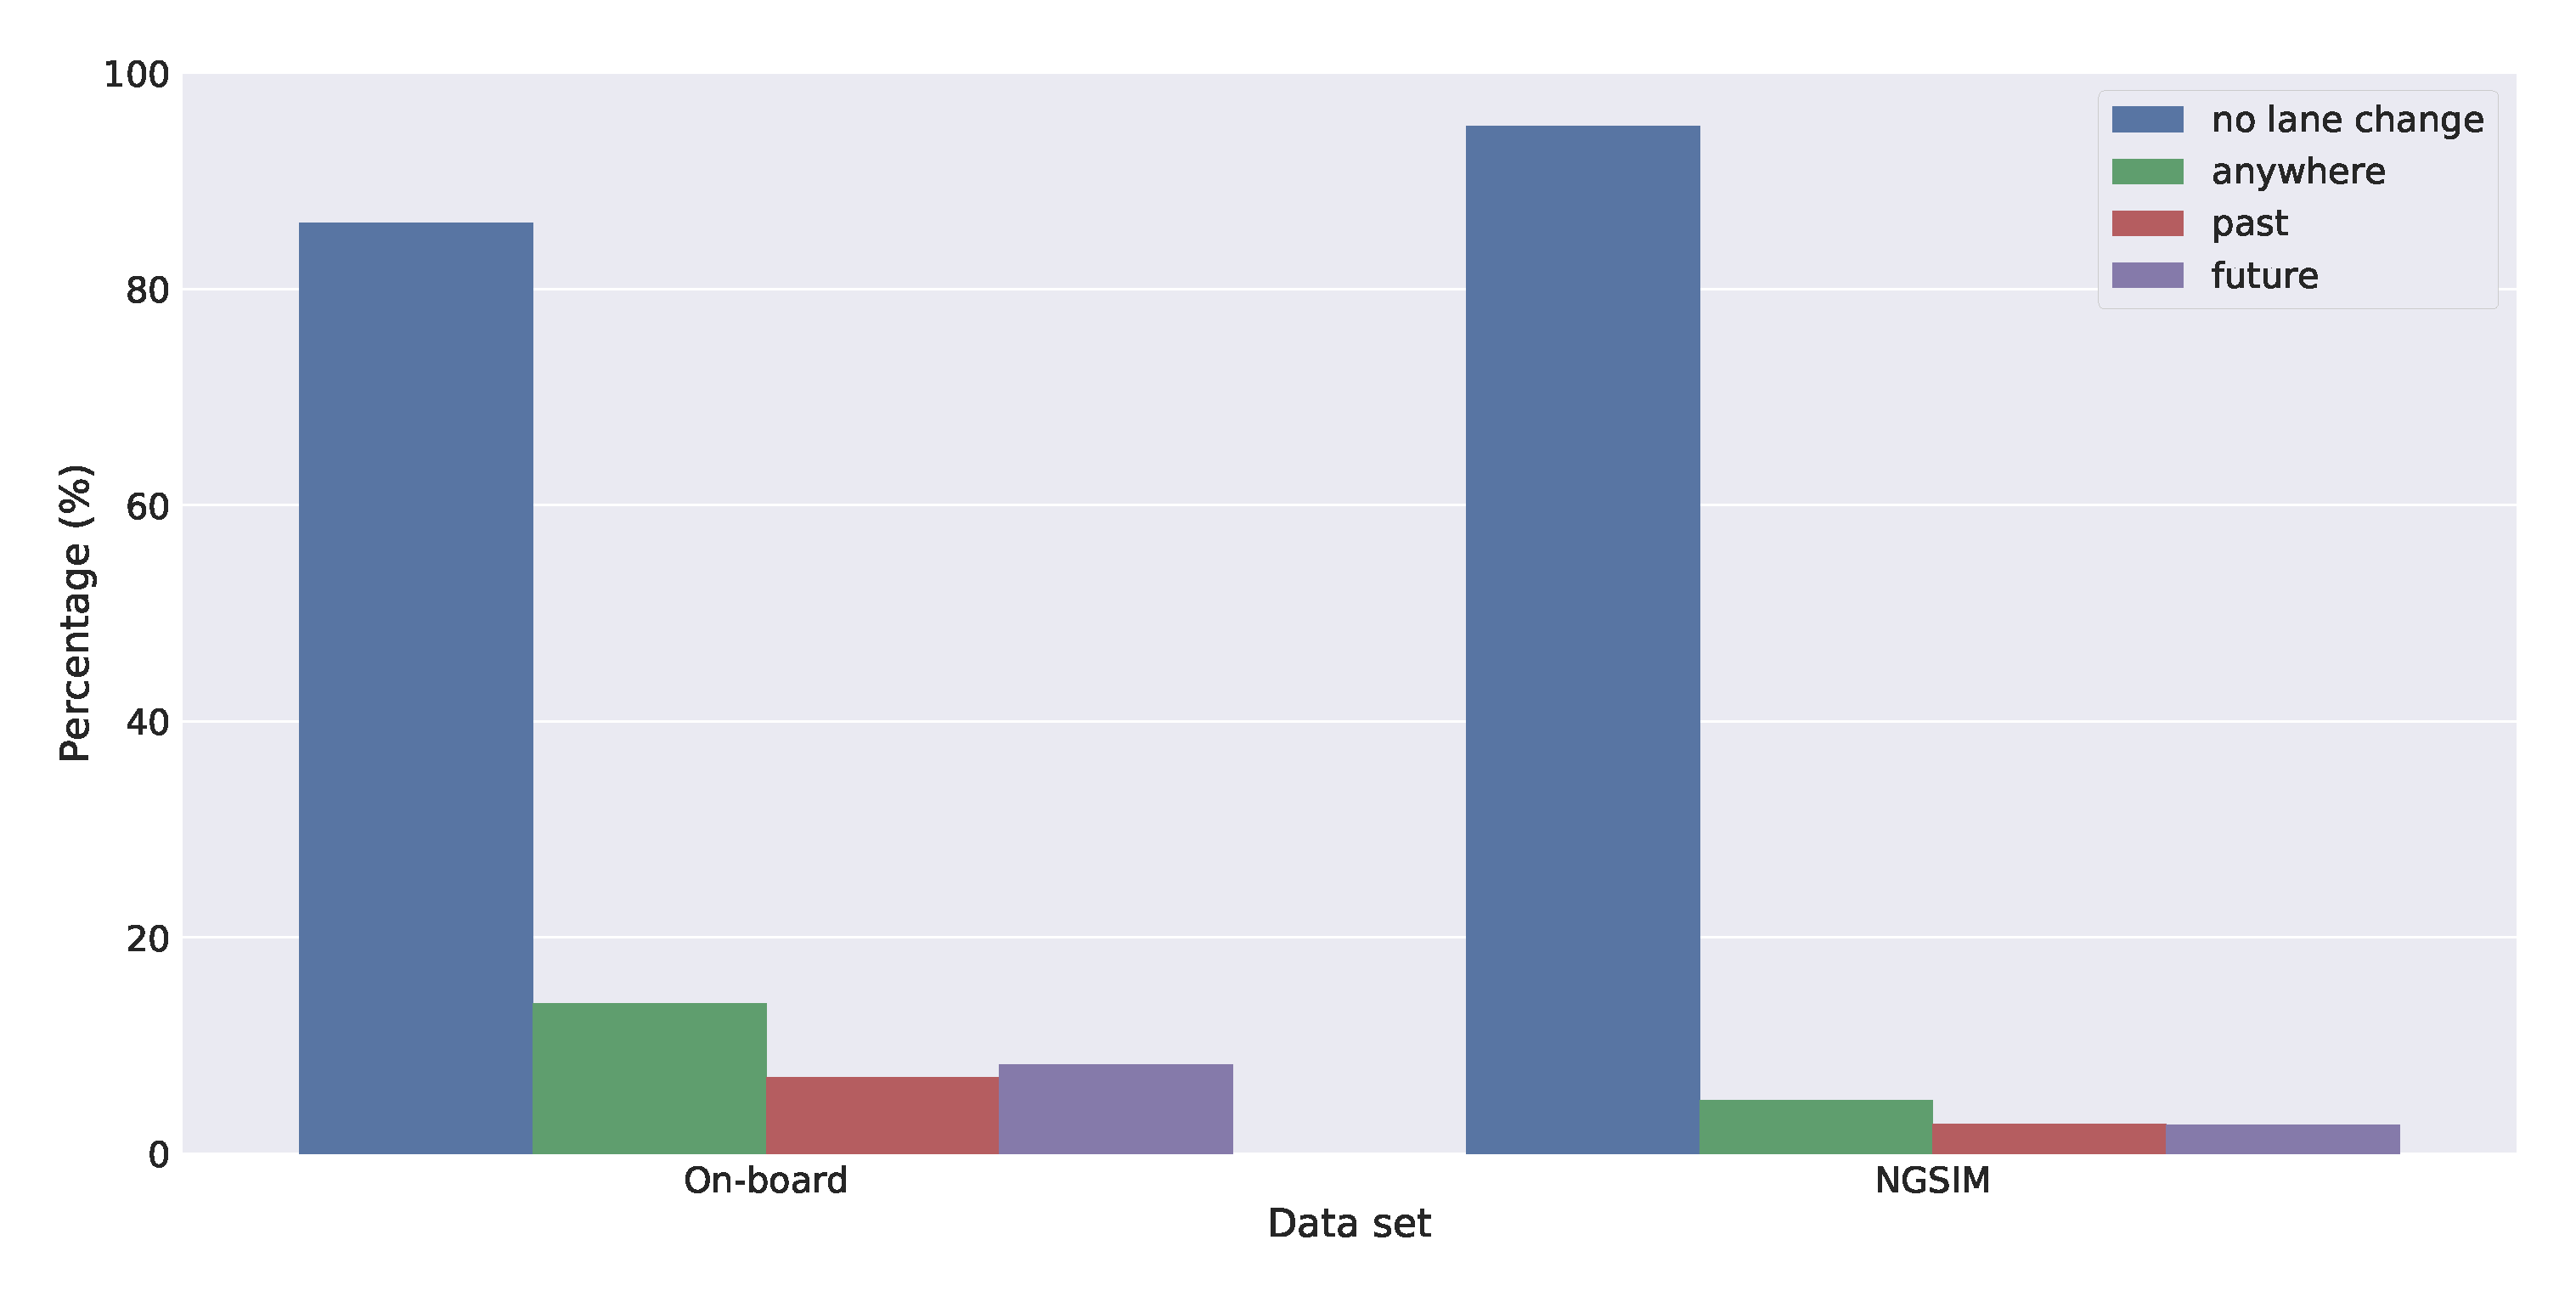
\includegraphics[width=1.\linewidth]{imgs/data_set_lane_change_distribution.eps}
    \caption{Visualization of the composition of both data sets regarding lane changes of the target vehicle.}
    \label{fig:data_set_lane_change_distribution}
\end{figure}

Figure~\ref{fig:data_set_lane_change_distribution} shows the amount of situations where the target vehicle performs a lane change in comparison to the amount of situations where no such behavior occurs for both, the \emph{On-board} and \emph{\ac{NGSIM}} data set.
For the \emph{On-board} data set, in \SI{86.1}{\percent} of all data samples the target vehicle does not perform a lane, i.e., only \SI{13.8}{\percent} of all data samples contain a lane change performed by the target vehicle.
We further distinguish between lane changes performed during the trajectory history, i.e., the past \SI{5}{\second} before the current time step (labeled as \emph{past} in Fig.~\ref{fig:data_set_lane_change_distribution}) and lane changes that are performed in the future, i.e., during the future \SI{5}{\second} from the current time step (labeled as \emph{future} in Fig.~\ref{fig:data_set_lane_change_distribution}).
We consider the lane changes in the future part of data samples to be the most interesting and challenging ones, since any model making predictions about the future trajectory needs to be able to anticipate these lane changes.
For the \emph{On-board} data set, \SI{7}{\percent} of all data samples contain a lane change in the trajectory history, while \SI{8.2}{\percent} of the samples contain a future lane change performed by the target vehicle.
In comparison to the \SI{86.1}{\percent} of data samples not containing a lane change, the amount of samples with interesting behavior other than straight driving within the data set is significantly less present.
For the \emph{\ac{NGSIM}} data set, the discrepancy between the amount of samples without the target vehicle performing lane change and the number of samples containing a lane change is even more significant.
The percentage of samples without a target vehicle lane change is \SI{95.1}{\percent} while only \SI{4.9}{\percent} of the samples contain a lane change performed by the target vehicle at all.
The amount of samples containing a future lane change performed by the target vehicle is only \SI{2.6}{\percent} of all samples in the \emph{\ac{NGSIM}} data set.
Hence, there is a significant imbalance in both data sets between examples containing mainly straight driving by the target vehicle, namely \SI{86.1}{\percent} and \SI{95.1}{\percent} of all samples in the \emph{On-board} and \emph{\ac{NGSIM}} data set respectively, where most likely already simple prediction approaches are able to achieve reasonable results.

\subsection{Performance baselines}
\label{subsec:baselines}

\begin{figure}[th!]
	\centering
	\subfloat[Overtaking maneuvre at $t=\SI{90}{\second}$\label{subfig:overtaking1}]{%
		\includegraphics[clip,width=\columnwidth]{imgs/Vis_overtaking_maneuvre_t1.png}
	}
	\vspace{-0.3cm}
	\subfloat[Overtaking maneuvre at $t=\SI{94}{\second}$\label{subfig:overtaking2}]{%
		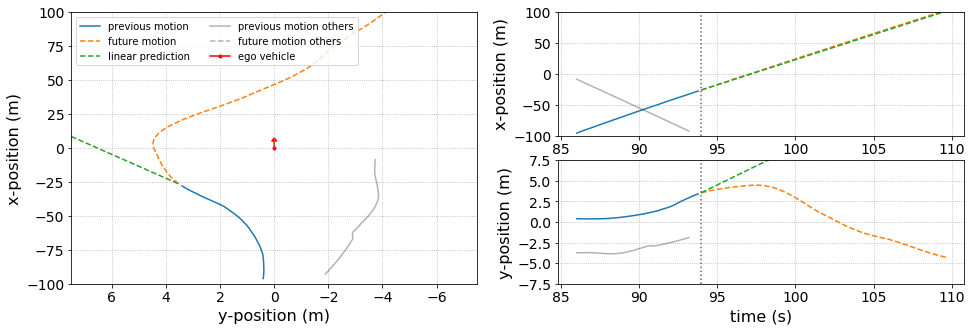
\includegraphics[width=\columnwidth]{imgs/Vis_overtaking_maneuvre_t2.png}
	}
	\vspace{-0.3cm}
	\subfloat[Overtaking maneuvre at $t=\SI{98}{\second}$\label{subfig:overtaking3}]{%
			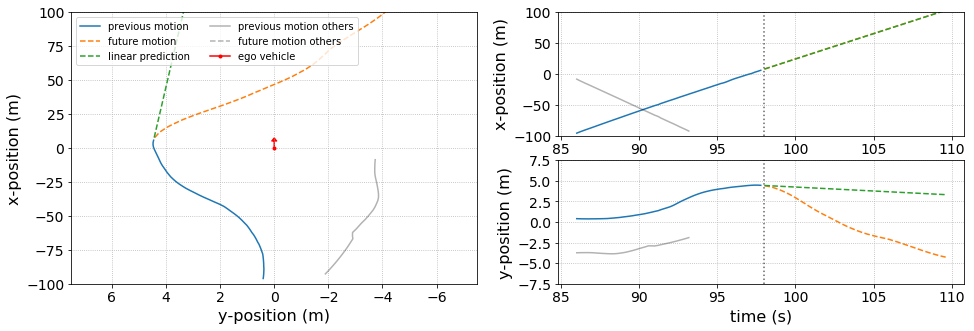
\includegraphics[width=\columnwidth]{imgs/Vis_overtaking_maneuvre_t3.png}
	}
	\vspace{-0.3cm}
	\subfloat[Overtaking maneuvre at $t=\SI{100}{\second}$\label{subfig:overtaking4}]{%
			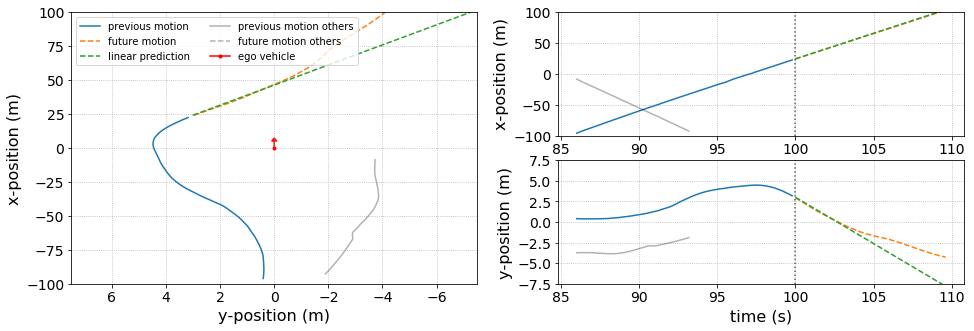
\includegraphics[width=\columnwidth]{imgs/Vis_overtaking_maneuvre_t4.png}
	}
	\caption{An example scene visualizing the data of an overtaking maneuver in a highway situation at selected time steps.}
    \label{fig:overtaking}
\end{figure}

In this section, we present and discuss the models we aim to use as performance baselines for our \ac{SPA}-based trajectory prediction approaches.
Therefore, we begin with an example:
Figure~\ref{fig:overtaking} shows an overtaking maneuver in a highway situation from the \emph{On-board} data set at four different selected time steps.
The ego-vehicle is overtaken by another car, the target vehicle to be predicted, approaching from behind.
During that overtaking maneuver, the ego-vehicle itself performs a lane change from the middle to the most right of the three lanes.
Figures~\ref{subfig:overtaking1}--~\ref{subfig:overtaking4} show different times of the situation.
Solid lines indicate previous positions whereas dashed lines indicate future positions or predictions.
The solid blue line depicts the past motion of the target vehicle overtaking the ego-vehicle, while solid gray lines visualize the past positions of other vehicles in the scene.
The dashed green line illustrates predictions from a simple linear model based on a constant velocity assumption.
This example illustrates the general trend we observe for both data sets used in this chapter that already simple linear prediction models achieve solid prediction accuracy, especially in $x$-direction.
This makes sense as both data sets almost exclusively contain highway driving situations, which in turn consists of significantly more straight driving and rather rare lane-change maneuvers as analyzed in section~\ref{subsec:data_set_peculiarities}.
For straight driving, linear prediction based on a constant velocity assumption is already a solid prediction approach, especially if all dynamic information (position, velocity etc.) is given relative to an already moving ego-vehicle like with the \emph{On-board} data set $D_1$.
Hence, we use these linear prediction models based on a constant velocity assumption as the simplest baseline models to compare our neural models using our distributed vector representations as input.

The analysis of related research on trajectory prediction in automotive context given in section~\ref{subsec:trajectory_prediction} suggests, that the most successful current state-of-the-art approaches rely mainly on \ac{LSTM}-based neural network architectures.
They are typically combined with other neural networks such as convolutional layers or classification networks \parencite{Deo2018a} to improve model performance.
In this chapter, we use \ac{LSTM}-based models as well as simpler feed-forward neural networks to predict trajectories based on our semantic vector representation of the current driving situation.
Hence, we use the same models just employing a different encoding (see section~\ref{subsec:scene_representation_in_vectors} for further details on the reference encoding schemes) of the input data avoiding further complexity of additional networks or layers to make the models as comparable as possible.

\section{Representation and models}
\label{sec:repr_models}

In this section, we describe the models we use for the behavior prediction task.
The input data for our models are sequences of positional data either as raw numerical values or in the form of semantic vectors as described in section~\ref{subsec:scene_representation_in_vectors}.
\ac{LSTM}-based neural network architectures have proven to be powerful tools for sequential data analysis and are widely used for behavior, or more generally, motion prediction.
We also investigate much simpler feed-forward neural networks constructed using the principles of the \acf{NEF} (c.f.\ section~\ref{sec:neural_eng}) to evaluate the performance gains achieved by the more complex \ac{LSTM} models.
To encode spatial information of driving situations in sequences of semantic vectors of fixed length, we employ the convolutive vector power introduced in Definition~\ref{def:conv_power} and analyzed in sections~\ref{subsec:different_vector_representations_for_numerical_values} and~\ref{subsec:capacity_analysis_limitations_to_vector_representations}.
For reference, we also describe a simpler vector representation employing the scalar multiplication encoding of numerical values also shown in section~\ref{subsec:different_vector_representations_for_numerical_values} as well as a raw numerical representation encoding only the positional information of the target vehicle.  
Furthermore, we describe the architecture of the learning models used for behavior prediction from that input data.
Importantly, here we use our models to predict one particular target vehicle at a time instead of trying to jointly predict the progress of the entire scene.
To achieve a forecast of the development of all vehicles in the scene, we would deploy several instantiations of the same network.
Using this approach, we only have to train one model while we can use each detected vehicle as training example, which significantly increases the amount of training data. 

\subsection{Scene representation in vectors}%
\label{subsec:scene_representation_in_vectors}

We use three different encoding schemes of the positional input data in this chapter.
Our main encoding scheme is the semantic vector representation as depicted in the following section making use of the convolutive vector power to encode numerical values (see also section~\ref{subsec:different_vector_representations_for_numerical_values}).
We also apply two other encoding schemes using the scalar multiplication encoding of numerical values in vectors (see also~\ref{subsec:different_vector_representations_for_numerical_values} as well as simply using the raw numerical values of the input data.

\subsubsection{Convolutive power representation}%
\label{ssubsec:convolutive_power_representation}

\begin{figure}[t!]
  \centering
  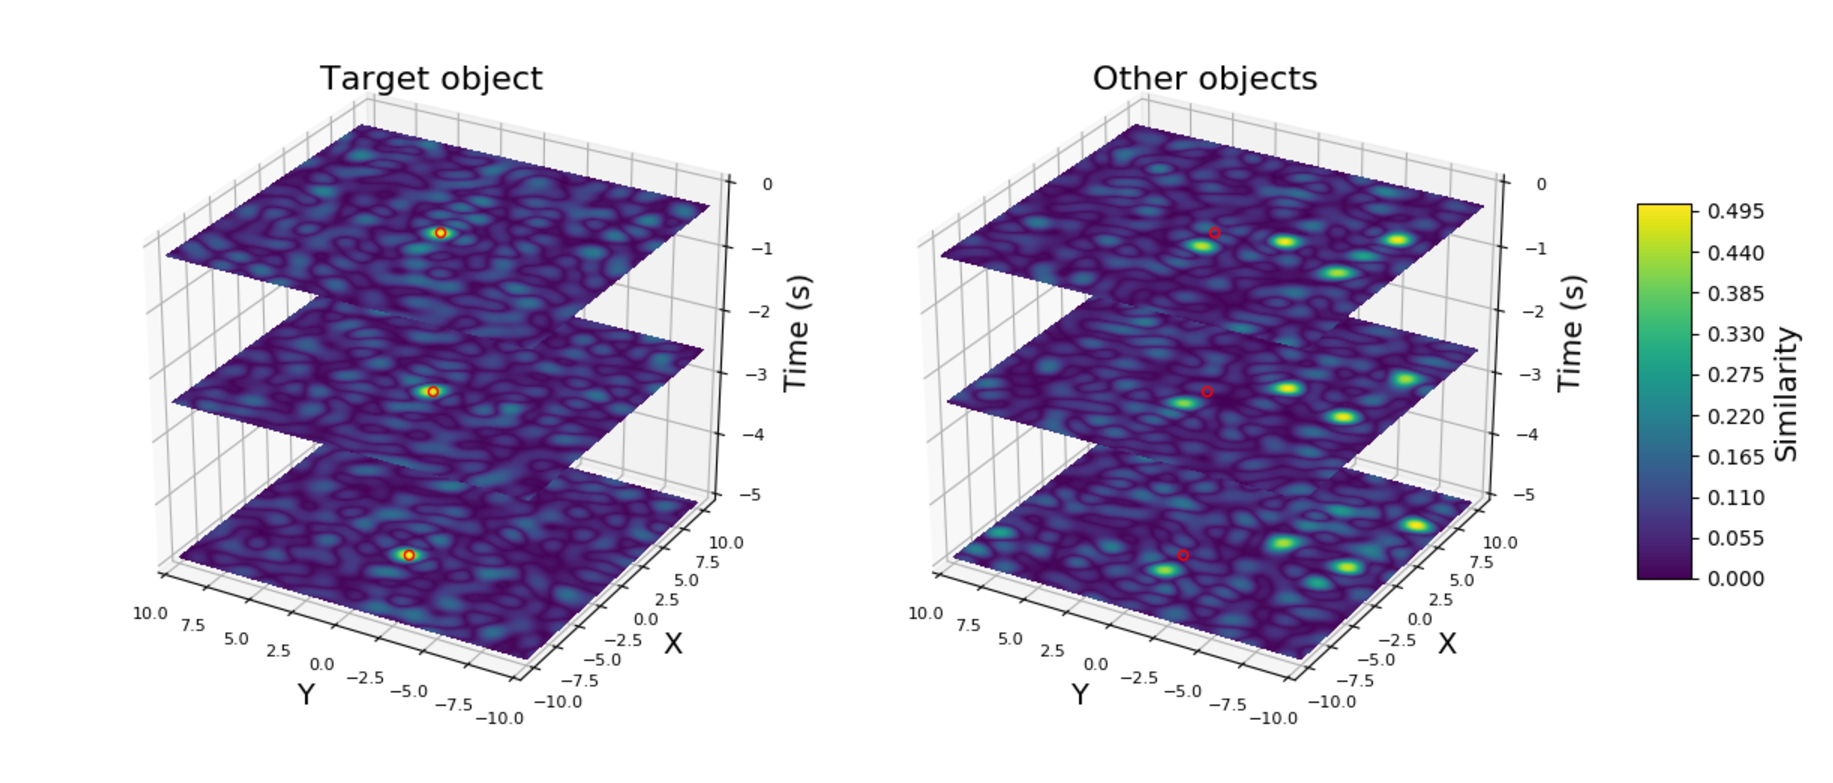
\includegraphics[width=0.95\textwidth]{imgs/spa_power_representation_in_time_viridis.eps}
  \caption{Visualization of the convolutive vector-power representation of one particular driving situation over time at selected time-steps as a heat map of similarity values for \num{512}-dimensional vectors. 
  The red circles indicate the measured position of the target vehicle.}
  \label{fig:spa_power}
\end{figure}

In this section, we investigate the expressive power of encoding the spatial positions of multiple vehicles using the convolutive vector-power introduced in Definition~\ref{def:conv_power}.
Given the results of section~\ref{subsec:the_influence_of_varying_vocabularies} that the impact of similarity structures in rather small vocabularies is neglectable, we create a random vocabulary $V$ of atomic vectors here.
We assign a random real-valued vector from the unit sphere to each category of dynamic objects (e.g.\ car, motorcycle, truck) as well as random unitary vectors (c.f.\ Definition~\ref{def:unitary_vec}) $\mathbf{X}$ and $\mathbf{Y}$ to encode the units of spatial positions in vectors.
We use unitary vectors $\mathbf{X}$ and $\mathbf{Y}$ since they have unit length and are closed under convolutive exponentiation as shown in Lemma~\ref{lemma:unitary_vec}.
Therefore, by encoding spatial positions with powers of unitary vectors, we avoid exploding lengths of our final scene vectors, which would lead to additional noise and unwanted behavior when using them as input for neural networks.
Furthermore, we use additional random ID-vectors $\mathbf{TARGET}$ and $\mathbf{EGO}$ representing the target object to be predicted and, if applicable, the ego-vehicle.
Given a situation as shown in Fig.~\ref{fig:on_board_data_example} with a sequence of prior positions $(x_{t}, y_{t})$ for the target vehicle at time step $t \in \left\{t_{0}, \ldots, t_{N} \right\}$ and equivalent sequences $(x_{obj,t}, y_{obj,t})$ for other traffic participants, we encapsulate this information in a scene vector

\begin{equation}
	\label{eq:conv_power_enc}
  \mathbf{S}_{t} = \underbrace{\mathbf{TARGET}\varoast \mathbf{TYPE}_{target} \varoast \mathbf{X}^{x_{t}} \varoast \mathbf{Y}^{y_{t}}}_{\textrm{target-vehicle}} \oplus \underbrace{\sum_{obj} \mathbf{TYPE}_{obj} \varoast \mathbf{X}^{x_{obj,t}} \varoast \mathbf{Y}^{y_{obj,t}}}_{\textrm{other objects}},
\end{equation}

This yields a sequence of semantic scene vectors $\mathbf{S}_{t}$ for $t \in \left\{t_{0}, \ldots, t_{N} \right\}$ encoding the past spatial development of objects in the current driving situation.
An alternative option could be to simply sum up the vectors at each past time step to encode the complete motion history within a single vector.
However, given the results regarding the capacity of the convolutive power encoding shown in section~\ref{subsec:capacity_analysis_limitations_to_vector_representations}, we decided for a sequence of individual vectors instead, which is also a more suitable input to neural networks employing \ac{LSTM} units.
Figure~\ref{fig:spa_power} depicts the aforementioned scene vector representation: the left plots show similarities (depicted as heat map) between the vector $\mathbf{S}_{t}$ encoding the scene from Fig.~\ref{fig:on_board_data_example} and the vectors $ \mathbf{v}_{i}=\mathbf{TARGET}\varoast \mathbf{TYPE}_{target} \varoast \mathbf{X}^{\bar{x}_{i}} \varoast \mathbf{Y}^{\bar{y}_{i}}$ for a sequence of discrete position samples ${\bar{x}_{i}, \bar{y}_{i}}$.
Similarly, the right plots show similarities between $\mathbf{S}_{t}$ and $\mathbf{CAR} \varoast \mathbf{X}^{\bar{x}_{i}} \varoast \mathbf{Y}^{\bar{y}_{i}}$ visualizing all other objects in the scene of type \emph{car}.
Importantly, each vector in the sequence $ \mathbf{S}_{t}$, i.e., each plane in the sequence of heat maps shown in Fig.~\ref{fig:spa_power} is a spatial encoding vector of the type depicted Fig.~\ref{fig:spa_power_encoding}
Hence, we can encode spatial information of several different objects in a sequence of semantic vectors and reliably decode it back out.
This allows us to encode automotive scenes with varying number of dynamic objects in a vector representation of fixed dimension.
Note that by using this vector representation as input data for a neural network (or any other predictor), we predict the future position of one other traffic participant at a time.
The indication vector $\mathbf{TARGET}$ bound to the target vehicle, i.e., the object we want the model to predict, indicates the network the current focus.
To predict all objects present in a scene during deployment, multiple instantiations of the same network can be used.
Thereby, the amount of training data generated per file increases with the number of objects while we only need to train one network.

To avoid accumulation of noise in the vectors (cf.\ section~\ref{subsec:capacity_analysis_limitations_to_vector_representations}) while focusing on the vehicles most relevant for prediction, we only use objects closer than \SI{40}{\meter} to the target vehicle in the \emph{On-board} data set.
For the \emph{\ac{NGSIM}} data set $D_2$, we additionally include only objects on the same lane as the target vehicle and on adjacent lanes.
Thereby, we aim for consistency across both data sets and we keep the input data as comparable as possible to what a driving vehicle could be able to detect using its on-board sensors.

For the \emph{On-board} data set $D_1$, we use two different variants of this representation, which differ in that the ego-vehicle's position is used or excluded in the \emph{other objects} part of Equation~\eqref{eq:conv_power_enc}, yielding two sequences $(\mathbf{S}_{t}^{ego})_{t_0}^{t_N}$ and $(\mathbf{S}_{t})_{t_0}^{t_N}$.
We used \acs{Nengo}'s \ac{SPA} package for implementation and therefore refer to these two encoding schemes $(\mathbf{S}_{t})_{t_0}^{t_N}$ and $(\mathbf{S}_{t}^{ego})_{t_0}^{t_N}$ as \emph{\ac{SPA}-power} and \emph{\ac{SPA}-power-with-ego} respectively.
As the \emph{\ac{NGSIM}} data set $D_2$ does not contain an ego-vehicle, we only investigate the \emph{\ac{SPA}-power} encoding scheme there.

\subsubsection{Reference encoding schemes}%
\label{ssubsec:reference_encoding_schemes}

For a simple reference vector-representation, we employ the scalar multiplication encoding for numerical values shown in section~\ref{subsec:different_vector_representations_for_numerical_values}.
Therefore, we add the positional vectors $\mathbf{X}$ and $\mathbf{Y}$ scaled with the target vehicle's prior positions $(x_{t}, y_{t})$ at each time step $t$, yielding the sequence $\tilde{\mathbf{S}}_{t} =  x_{t} \cdot \mathbf{X} + y_{t}\cdot \mathbf{Y}$.
We refer to this simpler encoding scheme based on the scalar multiplication encoding as \emph{\ac{SPA}-simple}.
Finally, we also use plain numerical position values $p_t = (x_{t}, y_{t})$ as another reference encoding scheme of the input data to our learning models, which we refer to as \emph{numerical}.
Importantly, only the \emph{\ac{SPA}-power} representation variants $(\mathbf{S}_{t})_{t_0}^{t_N}$ and $(\mathbf{S}_{t}^{ego})_{t_0}^{t_N}$ contain positional information about vehicles other than the target.

\subsection{\acs{LSTM}-based prediction models}%
\label{subsec:lstm_based_prediction_models}

\begin{figure}[t!]
  \centering
  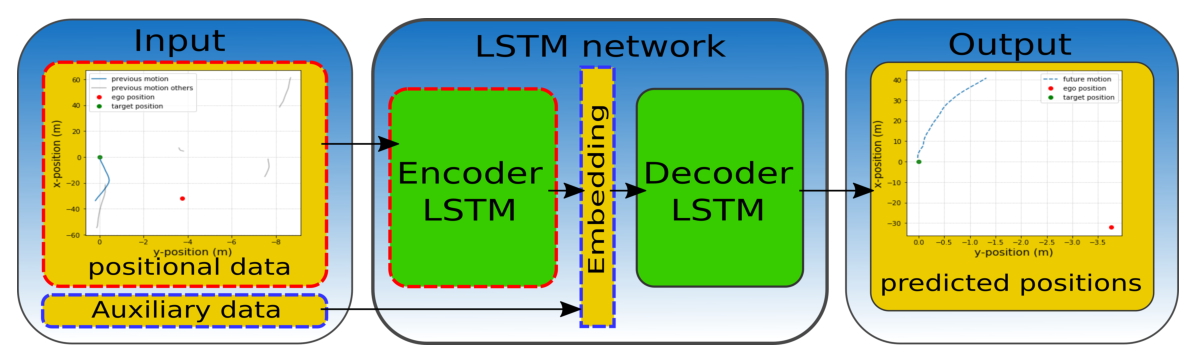
\includegraphics[width=0.95\textwidth]{imgs/lstm_arch.eps}
  \caption{Visualization of our \ac{LSTM}-based learning architecture. Modules that change with varying encoding scheme of the input data are highlighted through dashed red borders whereas parts that change when varying the data set are highlighted through dashed blue borders.}\label{fig:lstm_arch}
\end{figure}

In this section, we use a \acf{LSTM} \parencite{Hochreiter1997} network-architecture for the prediction of vehicle positions.
Our network consists of one \ac{LSTM} encoder and decoder cell for sequence to sequence prediction, which means that the input and the final result of our model is sequential data.
The encoder \ac{LSTM} takes positional data for $20$ past, equidistant time frames as input.
That is, the input data is a sequence of \num{20} items of either positions of the target vehicle or a sequence of high-dimensional vectors encoding this positional data.
The resulting embedding vector encodes the history of the input data over those time frames.
This embedding vector is concatenated with additional auxiliary information to aid the model when predicting the future trajectory of the target vehicle.
This auxiliary data is information, that is available to the system when the prediction is to happen, i.e., sensory data available at prediction time or future data about the ego-vehicle such as its own planned trajectory (see section~\ref{subsec:evaluation_of_the_lstm_based_prediction_models} for further details on this auxiliary data).
Finally, the embedding vector is used as input for the decoder \ac{LSTM} to predict future vehicle positions.
The output of each model is a sequence of \num{20} positions of the target vehicle predicted over a certain temporal horizon into the future.
We use the same network architecture for all encoding schemes of the input data and for both data sets.
However, the dimensionality of the input and the information used as auxiliary information to enrich the embedding vector vary over different encoding schemes and data sets respectively.
Figure~\ref{fig:lstm_arch} visualizes the architecture of our \ac{LSTM} models indicating modules that change when varying the encoding scheme by a dashed red border whereas parts that change with the data set are highlighted through a dashed blue border.

\subsection{Simple feed-forward \acs{NEF}-based prediction models}%
\label{subsec:simple_feed_forward_nef_based_prediction_models}

As an alternative to the \ac{LSTM}-models, we also considered a much simpler single-hidden-layer network defined using the \acf{NEF} \parencite{Eliasmith2003}.
While this is usually used for constructing large-scale biologically realistic neuron models \parencite{Eliasmith2012}, the \ac{NEF} software toolkit \acs{Nengo} \parencite{Bekolay2014} also allows for traditional feed-forward artificial neural networks using either spiking or non-spiking neurons.
For these \ac{NEF} networks, we use a single hidden layer, with randomly generated (and fixed) input weights, and use least-squares optimization to compute the output weights.
We employ the principles of the \ac{NEF} as shown in section~\ref{sec:neural_eng} to instantiate and train these models.
As with any traditional network, we can have any number of input, output, and hidden neurons, all following this same process.
The goal here is to provide a simple baseline for comparison to the \ac{LSTM} networks, to see what (if any) performance gain is produced by the more complex network approach.
However, these simpler networks are unable to process sequential data in the same way as the \ac{LSTM} models.
Therefore, we will have to slightly adapt our data, especially the semantic vector sequences, to make it suitable as input for the feed-forward networks.

\subsection{Excursion on unsupervised anomaly detection}%
\label{subsec:excursion_on_unsupervised_anomaly_detection}

In this section, we take a brief detour on anomaly detection.
We are further interested in the information encapsulated within our semantic vector representation and if it can be used to detect potentially dangerous driving situations from just the vector representation.
\acp{VSA} in general already have an intrinsic mechanism of comparing vectors with one another through the measure of similarity $\phi$.
However, it is not clear if simply comparing vectors in terms of similarity to, for instance, the mean pairwise-similarity of all known vectors, or a subset of vectors considered \enquote{normal}, will differentiate outliers from the \enquote{normal data}.
A-priori, it might not even be clear what vectors belong to the baseline set of normal data or how to define vectors to be considered as inliers.
One option could be to manually define metrics such as the number of vehicles in the scene or a threshold for the distance between the vehicles to detect crowded and potentially dangerous situations.
However, such an approach suffers from the typical issues of manual engineering such as biases introduced by the human designer as well as poor scaling.
Therefore, we employ an unsupervised learning approach based on fully-connected autoencoder neural networks similar to the one proposed in \textcite{Chen2017}.
We train an autoencoder neural network on the latest vector in the sequence $(\mathbf{S}_{t})_{t_0}^{t_N}$ of our scene vectors based on the convolutive vector-power representation in unsupervised fashion.
Thereby, the network is trained to reconstruct, i.e., generate replicates of, the data it is given.
Once the network is trained on a sufficiently large data set, we can calculate the element-wise error between the original vector $ \mathbf{v} = \left(v_{0}, \ldots, v_{D-1}\right)$ and the replicate vector $ \tilde{\mathbf{v}} = \left(\tilde{v}_{0}, \ldots, \tilde{v}_{D-1}\right)$ generated by the neural network autoencoder, i.e.,
\begin{equation}
\label{eq:anom_error}
\epsilon_{ \mathbf{v}} = \sqrt{ \frac{1}{D} \sum\limits_{i=0}^{D-1} \left(v_{i} - \tilde{v}_{i}\right)^{2}}.
\end{equation}
Vectors exceeding a certain threshold $c$ for this reconstruction error, i.e., $\epsilon_{ \mathbf{v}} > c$ will be considered as outliers or anomalies.
The threshold $c$ is generated from the percentage of examples we expect to be anomalies within the data set, which is typically chosen in the range of \SIrange{5}{15}{\percent}.

\section{Experiments and results}
\label{sec:experiments}

In this section, we describe the training process and parameters of all our models and give a detailed analysis and evaluation of the results achieved.
The \ac{LSTM} models are implemented in Tensorflow \parencite{Abadi2016} whereas the \ac{NEF} models are implemented using the \acs{Nengo} software suite \parencite{Bekolay2014}.
We use the \ac{RMSE} as our main metric for evaluation purposes.
In contrast to earlier work, we inspect the \ac{RMSE} for lateral and longitudinal directions separately to give more detailed insights into the models' behavior.
Calculating the \ac{RMSE} of the Euclidean distance would absorb the influence of the lateral \ac{RMSE} since it is an order of magnitude smaller than the longitudinal \ac{RMSE}, while we consider both directions to be at least equally important.
The lateral \ac{RMSE} is even more informative regarding the models' performance on, for instance, lane change maneuvers.
For all evaluations in this section, we refer to the longitudinal and lateral direction as $x$- and $y$-direction respectively.
Furthermore, we investigate where the models show their best performance looking for correlations between prediction accuracy and specific driving situations.

For both model types, we follow the same order of analyzing steps: firstly, we perform an investigation of the model's hyperparameters to find the best possible configuration for each model.
Secondly, we describe the process of training each model with all peculiarities corresponding to the data used or the training process itself.
Finally, we evaluate the trained models and compare their performance.
For the hyperparameter analysis, we conduct a thorough investigation on both our network architectures using only numerical input data for simplicity and to keep the time needed for training limited.
Systematically, we only analyze one parameter at a time and fix the best value for that parameter for the subsequent analysis of other parameters.
However, we also inspect certain parameter pairs jointly if there are correlations or mutual influences between the parameters to be expected.
All hyperparameter analyses in this section on both model types are performed on the \emph{On-board} data set $D1$.
If not declared otherwise, all figures show the performance of the investigated models on the validation part $V_1 \subset D_1$ of the \emph{On-board} data set.
The training process however is intended to be kept as coherent as possible between the data sets and differences having an impact on the training process will be highlighted where necessary.
Finally, we evaluate both model types' performance on both available data sets and, especially for the \ac{LSTM}-based models, we give a thorough analysis on which model performs best depending on the current driving context.
Thereby, we will identify strengths and weaknesses of each particular model.

\begin{center}
    \resizebox{\textwidth}{!}{%
        \begin{tabular}{cccccccc}
            \toprule
            \thead{Short name} & \thead{Input} & \thead{Position \\ encoding} & \thead{Network \\ architecture} & \thead{Training} & \thead{Number of \\ Units/Neurons} & \thead{Data set}\\ 
            \midrule
            linear & \makecell{current position \\ and velocity} & - & Linear regression & - & - & both \\ 
            \midrule
            LSTM numerical & sequence of positions & - & \makecell{\acs{LSTM} with one \\ encoder/decoder cell each} & \makecell{Offline, \\ backpropagation} & \makecell{\num{150} units \\ per cell} & both \\ \midrule
            LSTM \acs{SPA} \num{1} & semantic vector sequence & convolutive power & \makecell{\acs{LSTM} with one \\ encoder/decoder cell each} & \makecell{Offline, \\ backpropagation} & \makecell{\num{150} units \\ per cell} &both \\ 
            \midrule
            LSTM \acs{SPA} \num{2} & semantic vector sequence & scalar multiplication & \makecell{\acs{LSTM} with one \\ encoder/decoder cell each} & \makecell{Offline, \\ backpropagation} & \makecell{\num{150} units\\  per cell} &both \\ 
            \midrule
            LSTM \acs{SPA} \num{3} & semantic vector sequence & \makecell{convolutive power \\ incl.\ ego-vehicle} & \makecell{\acs{LSTM} with one \\ encoder/decoder cell each} & \makecell{Offline, \\ backpropagation} & \makecell{\num{150} units \\ per cell} &\emph{On-board} \\ 
            \midrule
            \acs{NEF} numerical & sequence of positions & - & \acs{NEF} Single-layer & \makecell{Offline, \\ least-squares} & \num{3000} neurons & both \\ 
            \midrule
            \acs{NEF} \acs{SPA} \num{1} & semantic vector sum & \makecell{convolutive power \\ incl.\ ego-vehicle} & \acs{NEF} Single-layer & \makecell{Offline, \\ least-squares} & \num{3000} neurons  &\emph{On-board} \\ 
            \midrule
            \acs{NEF} \acs{SPA} \num{2} & semantic vector sum & convolutive power & \acs{NEF} Single-layer & \makecell{Offline, \\ least-squares} & \num{3000} neurons &\emph{\ac{NGSIM}}\\ 
            \bottomrule
        \end{tabular}
    }
	\captionof{table}{Summary of the evaluated models regarding architecture, input data, encoding and training.}
	\label{tab:evaluated_models}
\end{center}

Table~\ref{tab:evaluated_models} summarizes the models evaluated in this section.
The models \ac{LSTM} \ac{SPA} \num{1} - \num{3} as well as \ac{LSTM} numerical employ the same network architecture as described in section~\ref{subsec:lstm_based_prediction_models} with sequential information as input data (using the different encoding schemes presented in section~\ref{ssubsec:reference_encoding_schemes}) and are analyzed in section~\ref{subsec:evaluation_of_the_lstm_based_prediction_models}.
The models \ac{NEF} \ac{SPA} \num{1} and \num{2} employ the simpler, single-layer, feed-forward architecture as described in section~\ref{subsec:simple_feed_forward_nef_based_prediction_models} with a vector obtained as partial sum of vectors from the whole sequence used as input for the \ac{LSTM} models (see section~\ref{subsec:evaluation_of_nef_based_feed_forward_prediction_models} for further details).
The models will be denoted in legends of the figures in this chapter by their short name given in table~\ref{tab:evaluated_models}.

In section~\ref{subsec:scene_representation_in_vectors}, we have described the different encoding schemes we will use to evaluate our models.
We mentioned that the models employing the convolutive power to encode the input data (i.e., \ac{LSTM} \ac{SPA} \num{1}, \num{3} and \ac{NEF} \ac{SPA} \num{1} and \num{2}) are the only ones having access to information about objects other than the target vehicle.
Although these models therefore have access to more data than the other reference models such as \ac{LSTM} numerical, we are interested in evaluating the benefits of encoding the interconnections between vehicles implicitly in the input data using our semantic vector encoding instead of introducing a more complex network architecture.
Therefore, we focus on the same network architecture for all encoding schemes in this chapter and leave a comparison with more sophisticated network architectures, for instance, ones combining \acp{LSTM} with social pooling layers as in \textcite{Deo2018a} or \textcite{Alahi2016} for future work.

\subsection{Evaluation of the \acs{LSTM}-based prediction models}%
\label{subsec:evaluation_of_the_lstm_based_prediction_models}

In this section, we will investigate the \ac{LSTM}-based prediction models.

\subsubsection{Hyperparameter analysis}%
\label{ssubsec:hyperparameter_analysis_lstms}

\begin{figure}[t!]
  \centering
  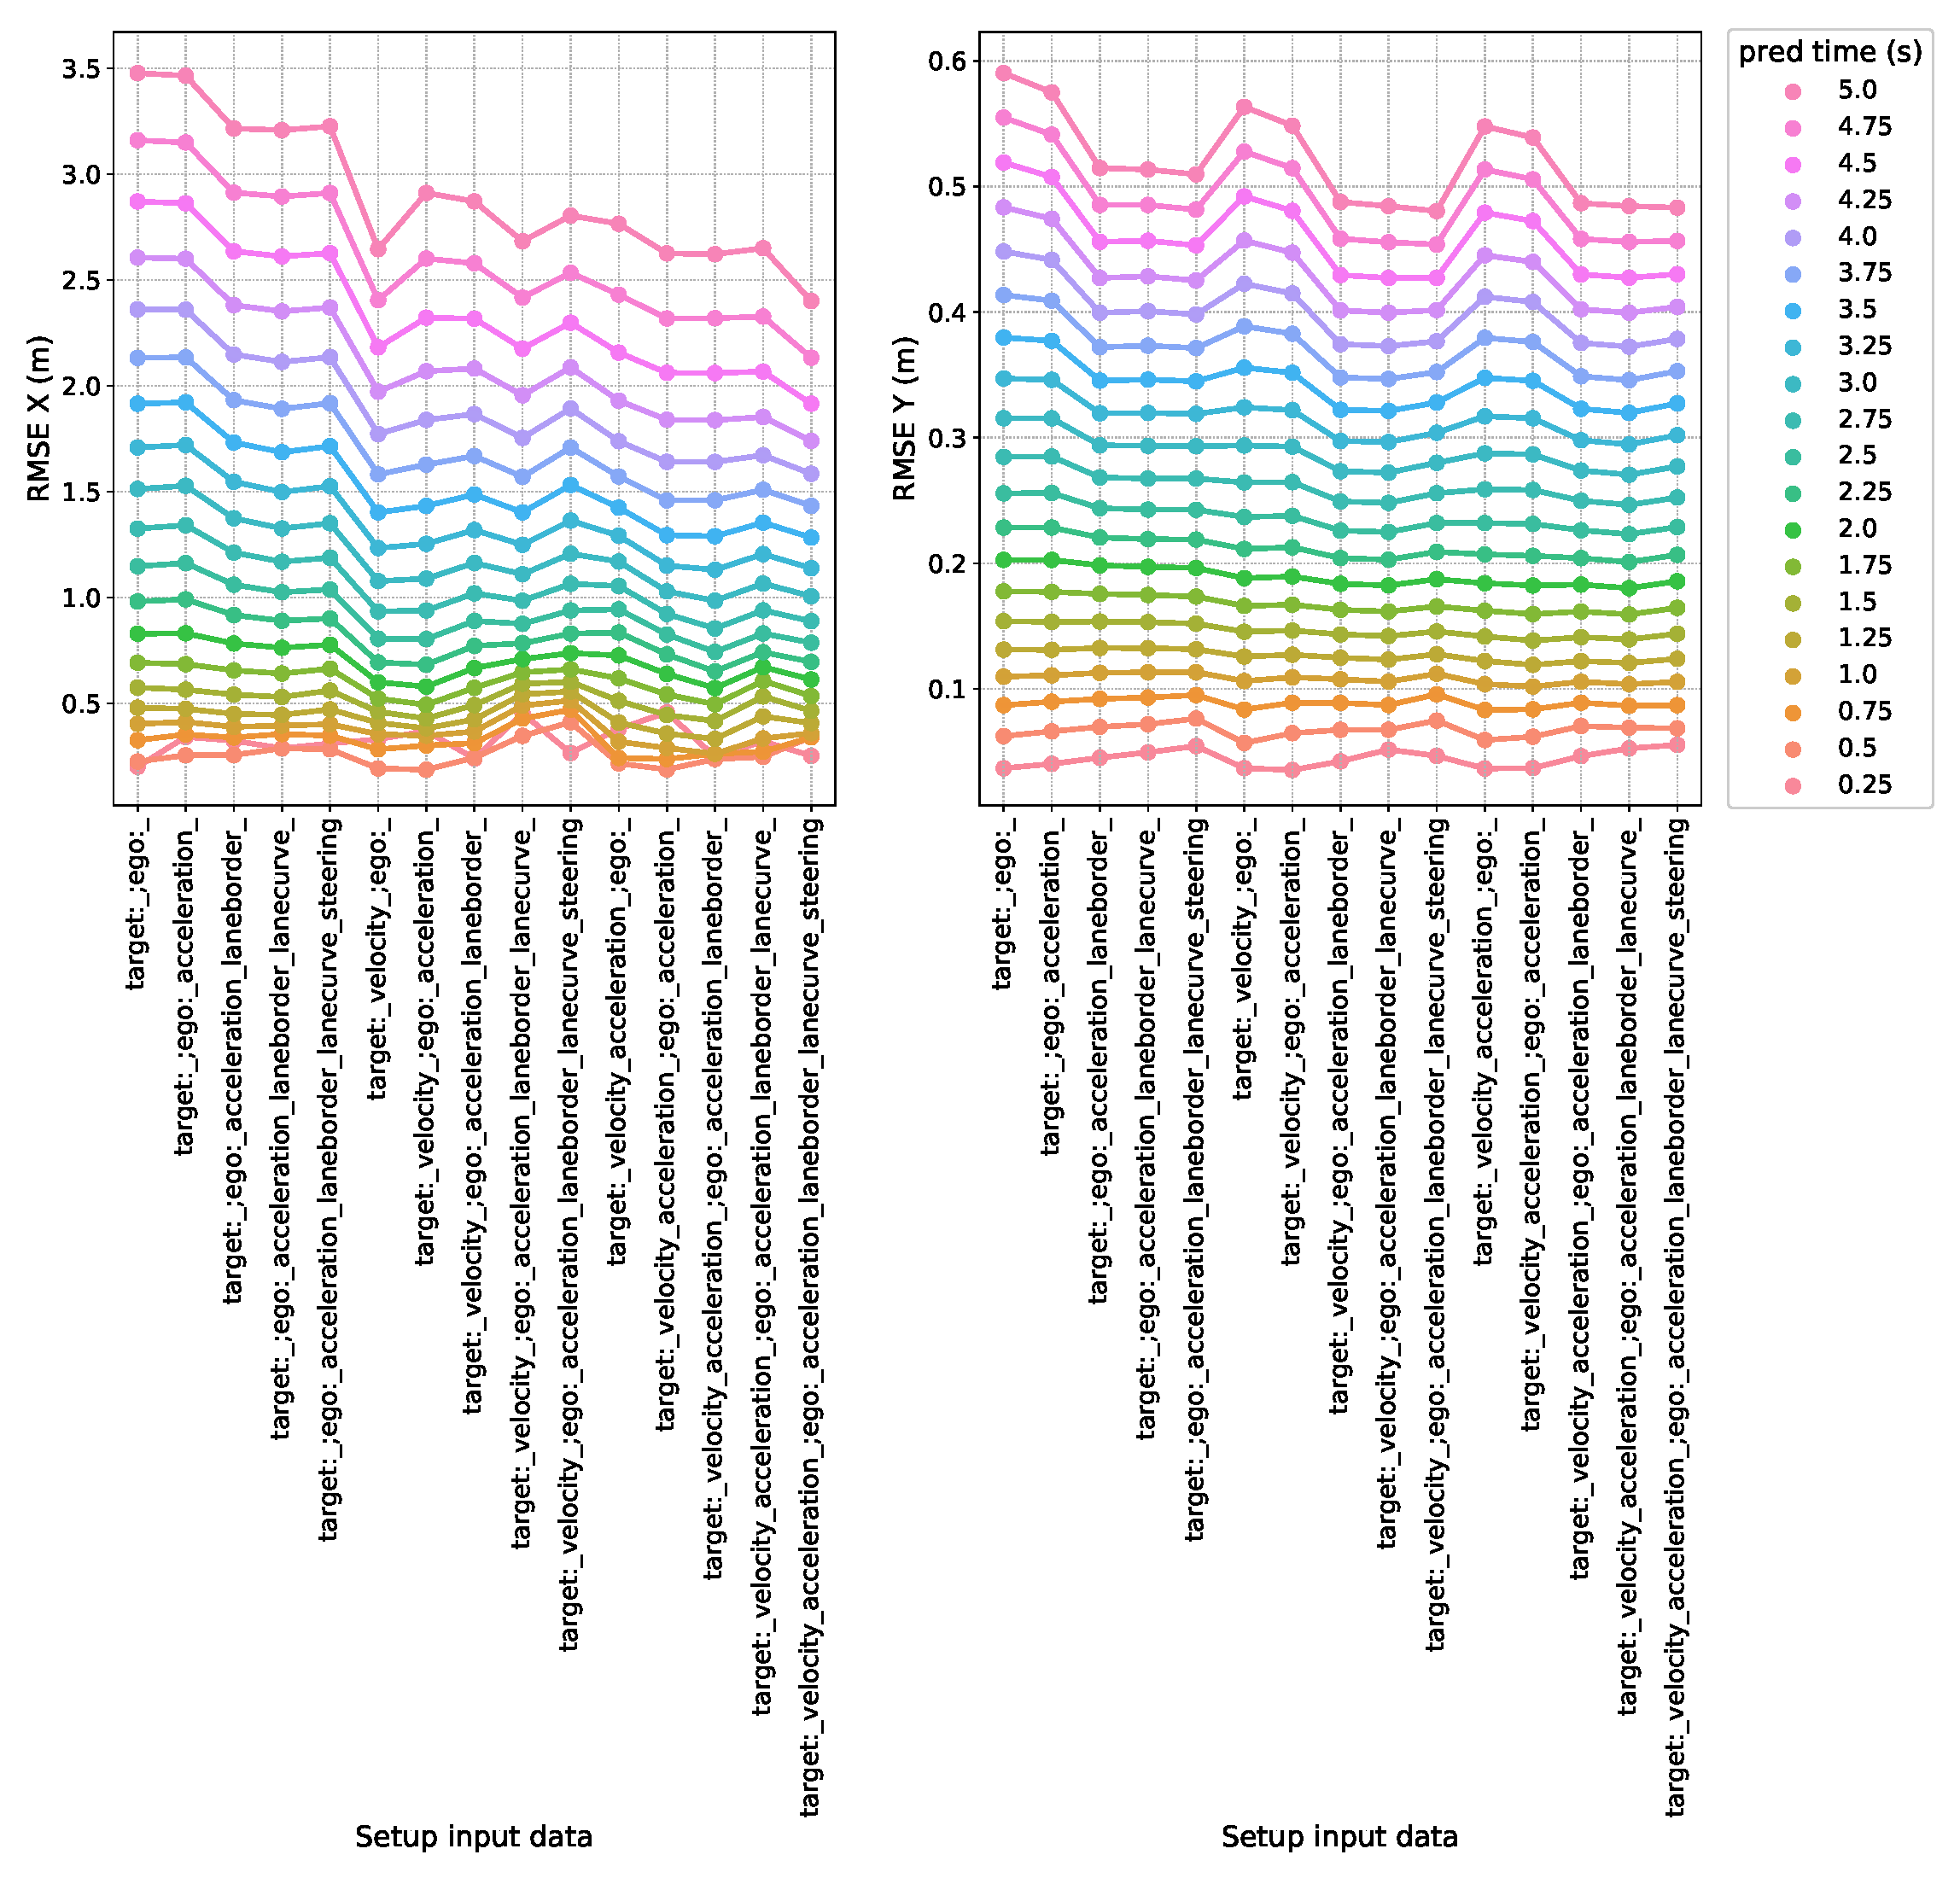
\includegraphics[width=0.95\textwidth]{imgs/lstm_input_data_analysis.eps}
  \caption{Analysis of the \ac{RMSE} for different variations of numerical input to our \ac{LSTM} model trained on the \emph{On-board} data set for \num{8} epochs.}
  \label{fig:lstm_input_data_analysis}
\end{figure}

\begin{center}
    \resizebox{\textwidth}{!}{%
        \begin{tabular}{cccccccc}
            \toprule
            \multirow{2}{1in}{\thead{Setup \#}} & \multicolumn{3}{c|}{\thead{Included target vehicle data}} & \multicolumn{4}{|c}{\thead{Included ego-vehicle data}} \\ 
            \cmidrule{2-8}
             & \thead{Position} & \thead{Velocity} & \thead{Acceleration} & \thead{Acceleration} & \thead{Lane Border} & \thead{Lane Curvature} & \thead{Steering}\\ 
            \midrule
            1 & \checkmark & & & & & &  \\
            \midrule
            2 & \checkmark & & & \checkmark& & &  \\
            \midrule
            3 & \checkmark & & & \checkmark& \checkmark& &  \\
            \midrule
            4 & \checkmark & & & \checkmark& \checkmark& \checkmark&  \\
            \midrule
            5 & \checkmark & & & \checkmark& \checkmark& \checkmark& \checkmark \\
            \midrule
            6 & \checkmark & \checkmark& & & & &  \\
            \midrule
            7 & \checkmark & \checkmark& & \checkmark& & &  \\
            \midrule
            8 & \checkmark & \checkmark& & \checkmark& \checkmark& &  \\
            \midrule
            9 & \checkmark & \checkmark& & \checkmark& \checkmark& \checkmark&  \\
            \midrule
            10 & \checkmark & \checkmark& & \checkmark& \checkmark& \checkmark& \checkmark \\
            \midrule
            11 & \checkmark & \checkmark& \checkmark& & & &  \\
            \midrule
            12 & \checkmark & \checkmark& \checkmark& \checkmark& & &  \\
            \midrule
            13 & \checkmark & \checkmark& \checkmark& \checkmark& \checkmark& &  \\
            \midrule
            14 & \checkmark & \checkmark& \checkmark& \checkmark& \checkmark& \checkmark&  \\
            \midrule
            15 & \checkmark & \checkmark& \checkmark& \checkmark& \checkmark& \checkmark& \checkmark \\
            \bottomrule
        \end{tabular}
    }
    \captionof{table}{Summary of the input data setups of the different models evaluated in Fig.~\ref{fig:lstm_input_data_analysis}.}
	\label{tab:input_data_setups}
\end{center}

For the \ac{LSTM}-models, we firstly investigated the composition of the input data to the model to get an idea, what kind of information is useful for the task of motion prediction.
Therefore, we trained several instantiations of our \ac{LSTM}-network architecture on the \emph{On-board} data set $D_1$ for different variations of the input data, for \num{8} epochs each.
Table~\ref{tab:input_data_setups} summarizes the different setups and shows what kind of data is included in each setup shown in Fig.~\ref{fig:lstm_input_data_analysis}.
The simplest setting (setup \num{1}) is using only the positional information of the target vehicle as input and its instantaneous velocity as additional information in the embedding without including any information about the ego-vehicle.
We refer to this setting as the default setting in this section.
In addition, we also analyze settings, where additional information like velocity (setups \num{6}-\num{15}) and acceleration (setups \num{11}-\num{15}) of the target vehicle are available to the system.
Furthermore, if all dynamic information is available relative to the ego-vehicle, there are other features that could be useful for motion prediction such as the current curvature of the road or the current velocity or steering values of the ego-vehicle itself.
For instance, if the ego-vehicle performs a lane change or the road bends, this will influence the relative motion of all other vehicles while this information most likely will not be available from just the positions of the target vehicle. 
On the other hand, if such information is available to the system, it would improve the model's capability of abstracting and inferring correlations between the available information in such situations.
In this evaluation, we include the history of the ego-vehicle's information to the input data and future values to the embedding, whereas we include additional information about the target vehicle to the input data only. 

\begin{figure}[t!]
	\centering
    \subfloat[\label{subfig:lstm_units_analysis}]{%
        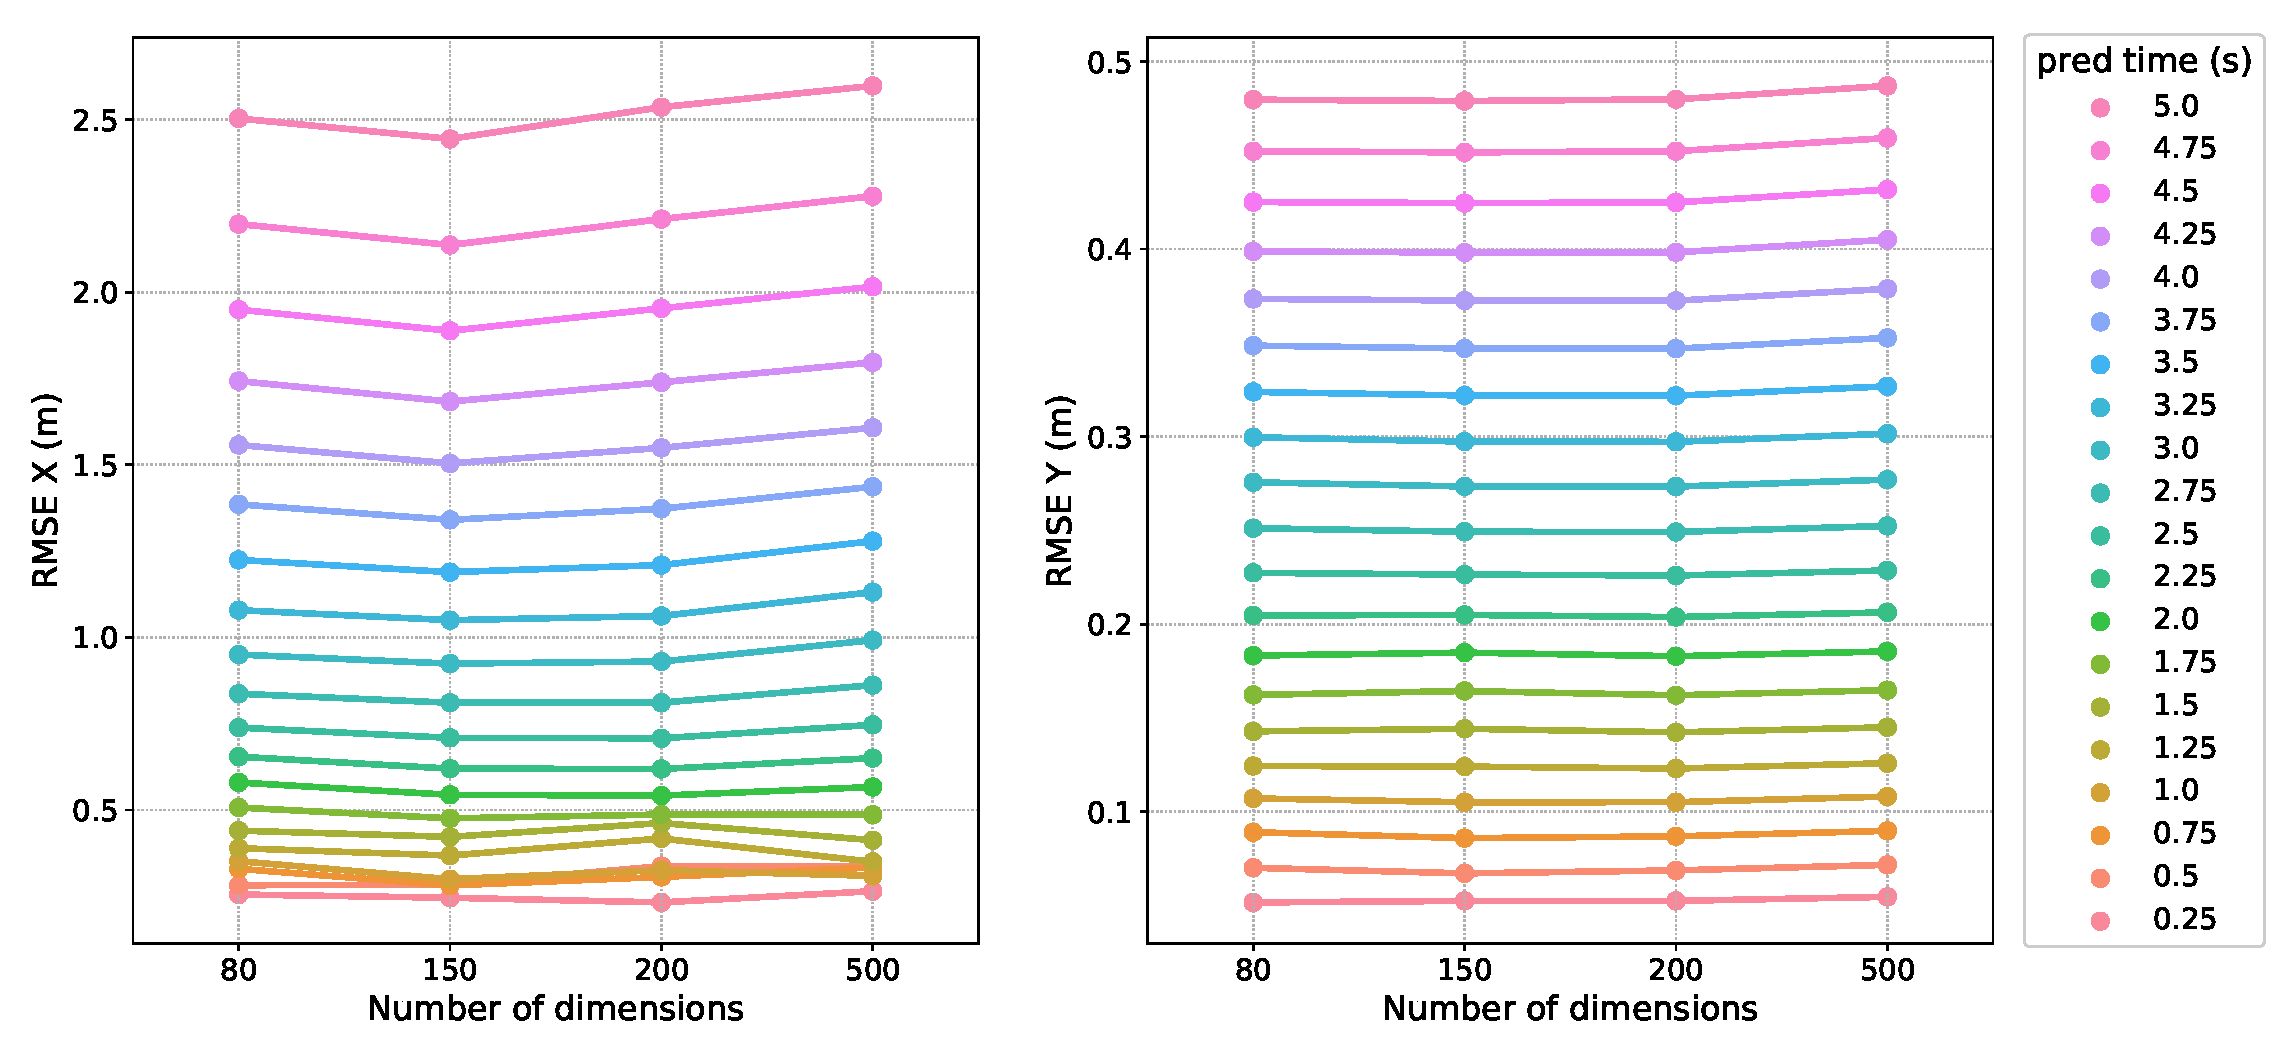
\includegraphics[width=\columnwidth]{imgs/lstm_units_analysis.eps}
    }
    \vspace{-0.3cm}
    \subfloat[\label{subfig:lstm_layers_analysis}]{%
        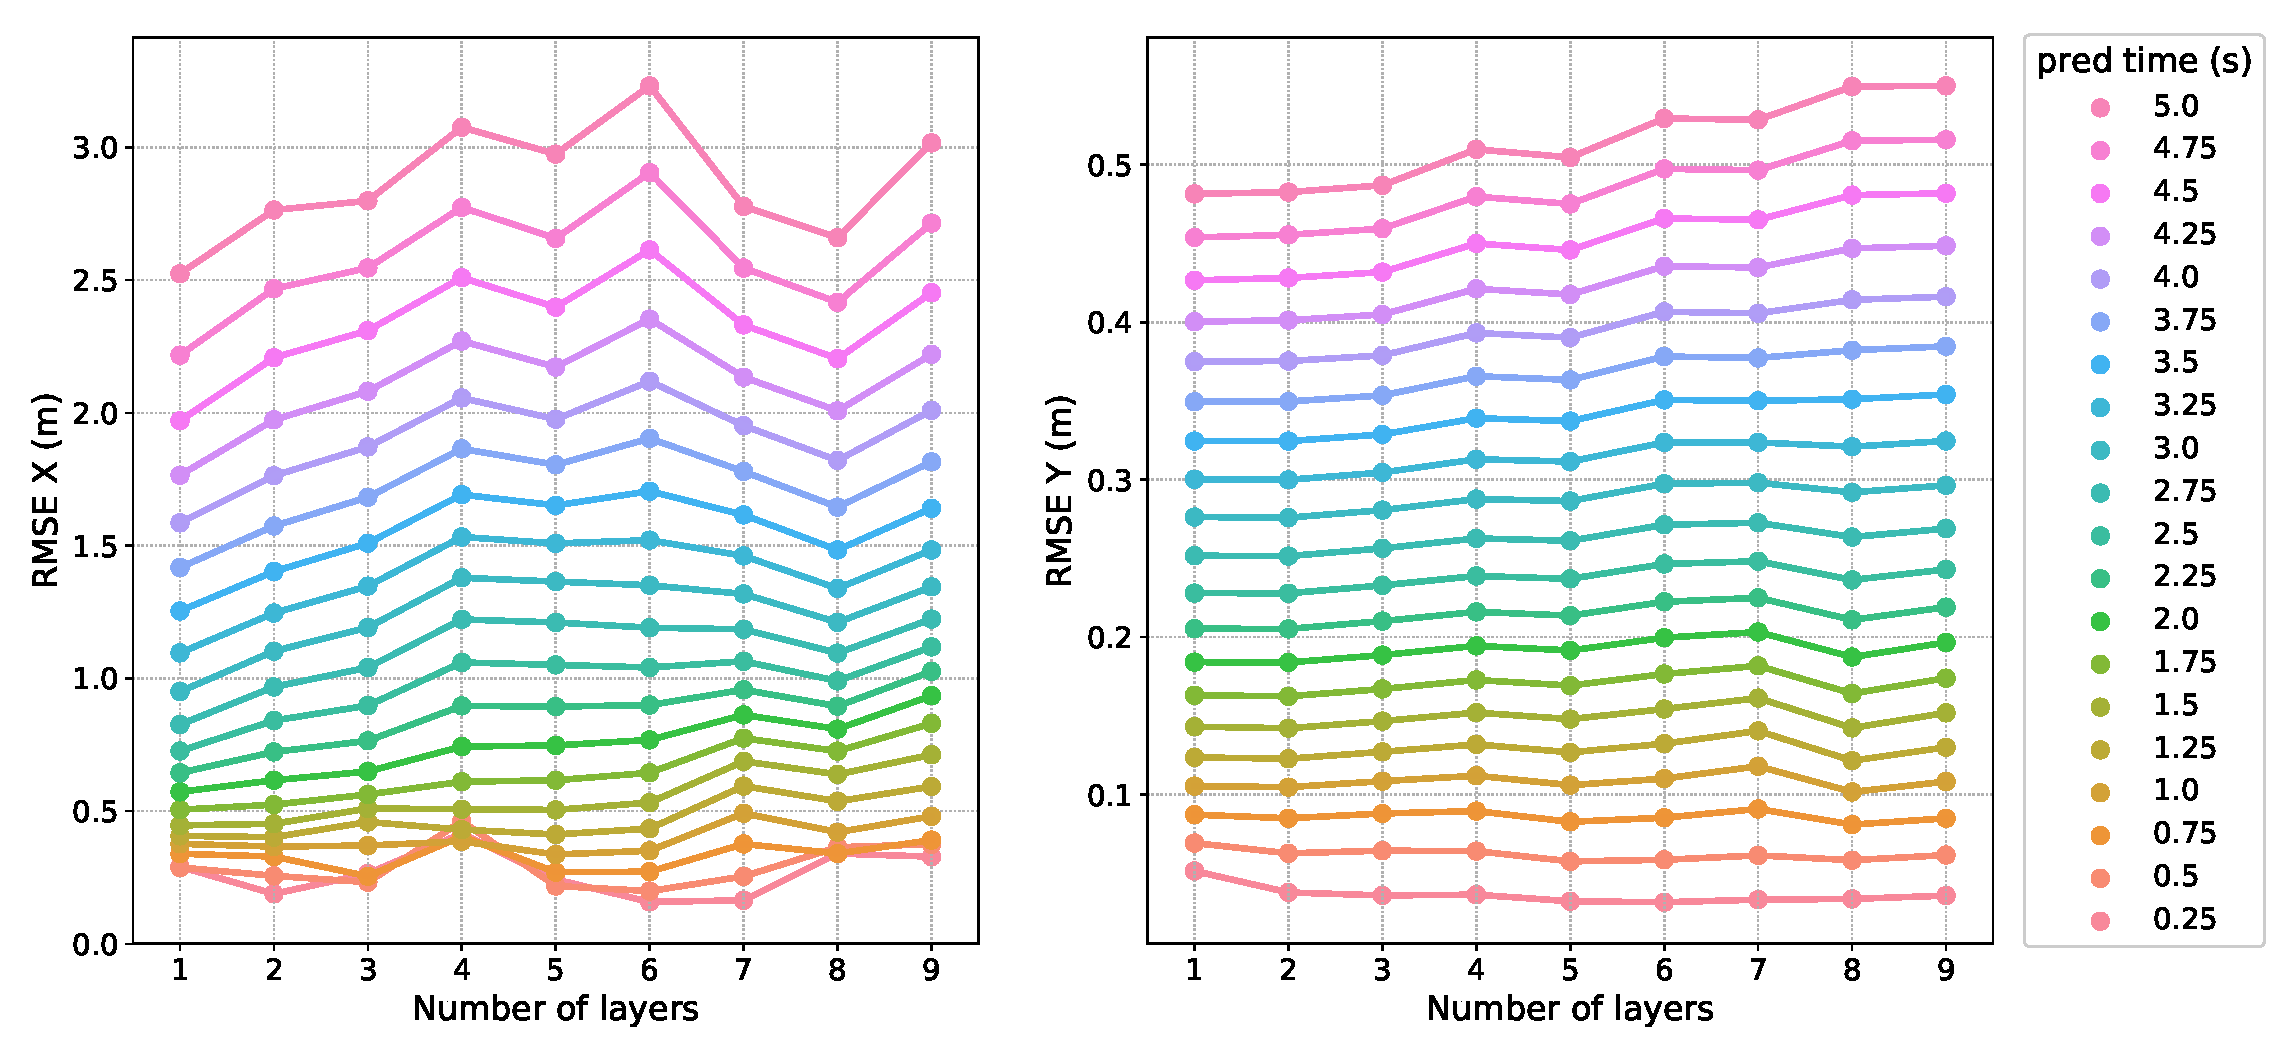
\includegraphics[width=\columnwidth]{imgs/lstm_layers_analysis.eps}
    }
    \caption{Visualization of the \ac{RMSE} for different parameter tests of our \ac{LSTM}-model trained on the \emph{On-board} data set for \num{8} epochs:~\protect\subref{subfig:lstm_units_analysis} depicts the \ac{RMSE} when varying the number of dimensions in each \ac{LSTM} cell~\protect\subref{subfig:lstm_layers_analysis} visualizes the \ac{RMSE} when varying the number of layers, i.e., the number of encoder and decoder \ac{LSTM} cells are used in the network.}
    \label{fig:lstm_units_layers_analysis}
\end{figure}

Figure~\ref{fig:lstm_input_data_analysis} depicts the \ac{RMSE} ($y$-axis) for each input data setup given in table~\ref{tab:input_data_setups} on the $x$-axis at each prediction time step.
Each tick on the $x$-axis corresponds to one input setup, whereas each group of \num{5} ticks from left to right corresponds to one fixed setup for the target vehicle.
The left group contains only the default data about the target vehicle (setups \num{1}-\num{5} in table~\ref{tab:input_data_setups}), the middle group contains the history of the target vehicle's velocity (setups \num{6}-\num{10} in table~\ref{tab:input_data_setups}) and the right group contains additionally the history of the target vehicle's acceleration (setups \num{11}-\num{15} in table~\ref{tab:input_data_setups}).
Each tick within one group corresponds to one setting for the ego-vehicle, whereas again from left to right the amount of available information increases.
Therefore, the rightmost tick contains information about the ego-vehicle's acceleration, distance to the lane border as well as the curvature of the current lane and its current steering values (setup \num{15} in table~\ref{tab:input_data_setups}). 
We observe that adding more information about both, the ego- and target vehicle, indeed improves prediction accuracy significantly: the difference between the best and worst setting is more than \SI{1}{\meter} in $x$-direction and more than \SI{0.1}{\meter} in $y$-direction.
For both dimensions, setup \num{15} using all available information outperforms the simpler setups.
However, there are some interesting peculiarities visible in this analysis that are worth noting.
For instance, the input information improving performance in $x$-direction the most appears to be the target vehicle's velocity (setups \num{1}-\num{5} vs. setups \num{6}-\num{10}). 
Furthermore, the target vehicle's acceleration does not yield further significant improvements given its velocity is available.
Interestingly, setup \num{6} using only the target vehicle's velocity as additional information is closely behind the best setting in $x$-direction.
Furthermore, the performance boost of the setting using all available information (setup \num{15} or the rightmost tick) over the prior setting comes from the ego-vehicle's steering, which only appears when its acceleration information is also available.
For the $y$-direction, we observe similar trends in that the target vehicle's acceleration does not yield significant improvements if its velocity is already given.
Here however, the information about the ego-vehicle's distance to the lane borders appears to be the input that gives the most significant improvements in $y$-direction (setup \num{2} vs. \num{3}, setup \num{7} vs. \num{8} and setup \num{12} vs. \num{13}).
That makes sense, since these inputs encode information about the ego-vehicle's motion in $y$-direction when, for instance, performing lane changes.
As setup \num{15} using all available information (the rightmost tick in Fig.~\ref{fig:lstm_input_data_analysis}) is by far outperforming all other settings in $x$-direction and is on par with the best in $y$-direction, we use this data setup for further analyzing the hyperparameters of the \ac{LSTM}-model.

\begin{figure}[t!]
  \centering
  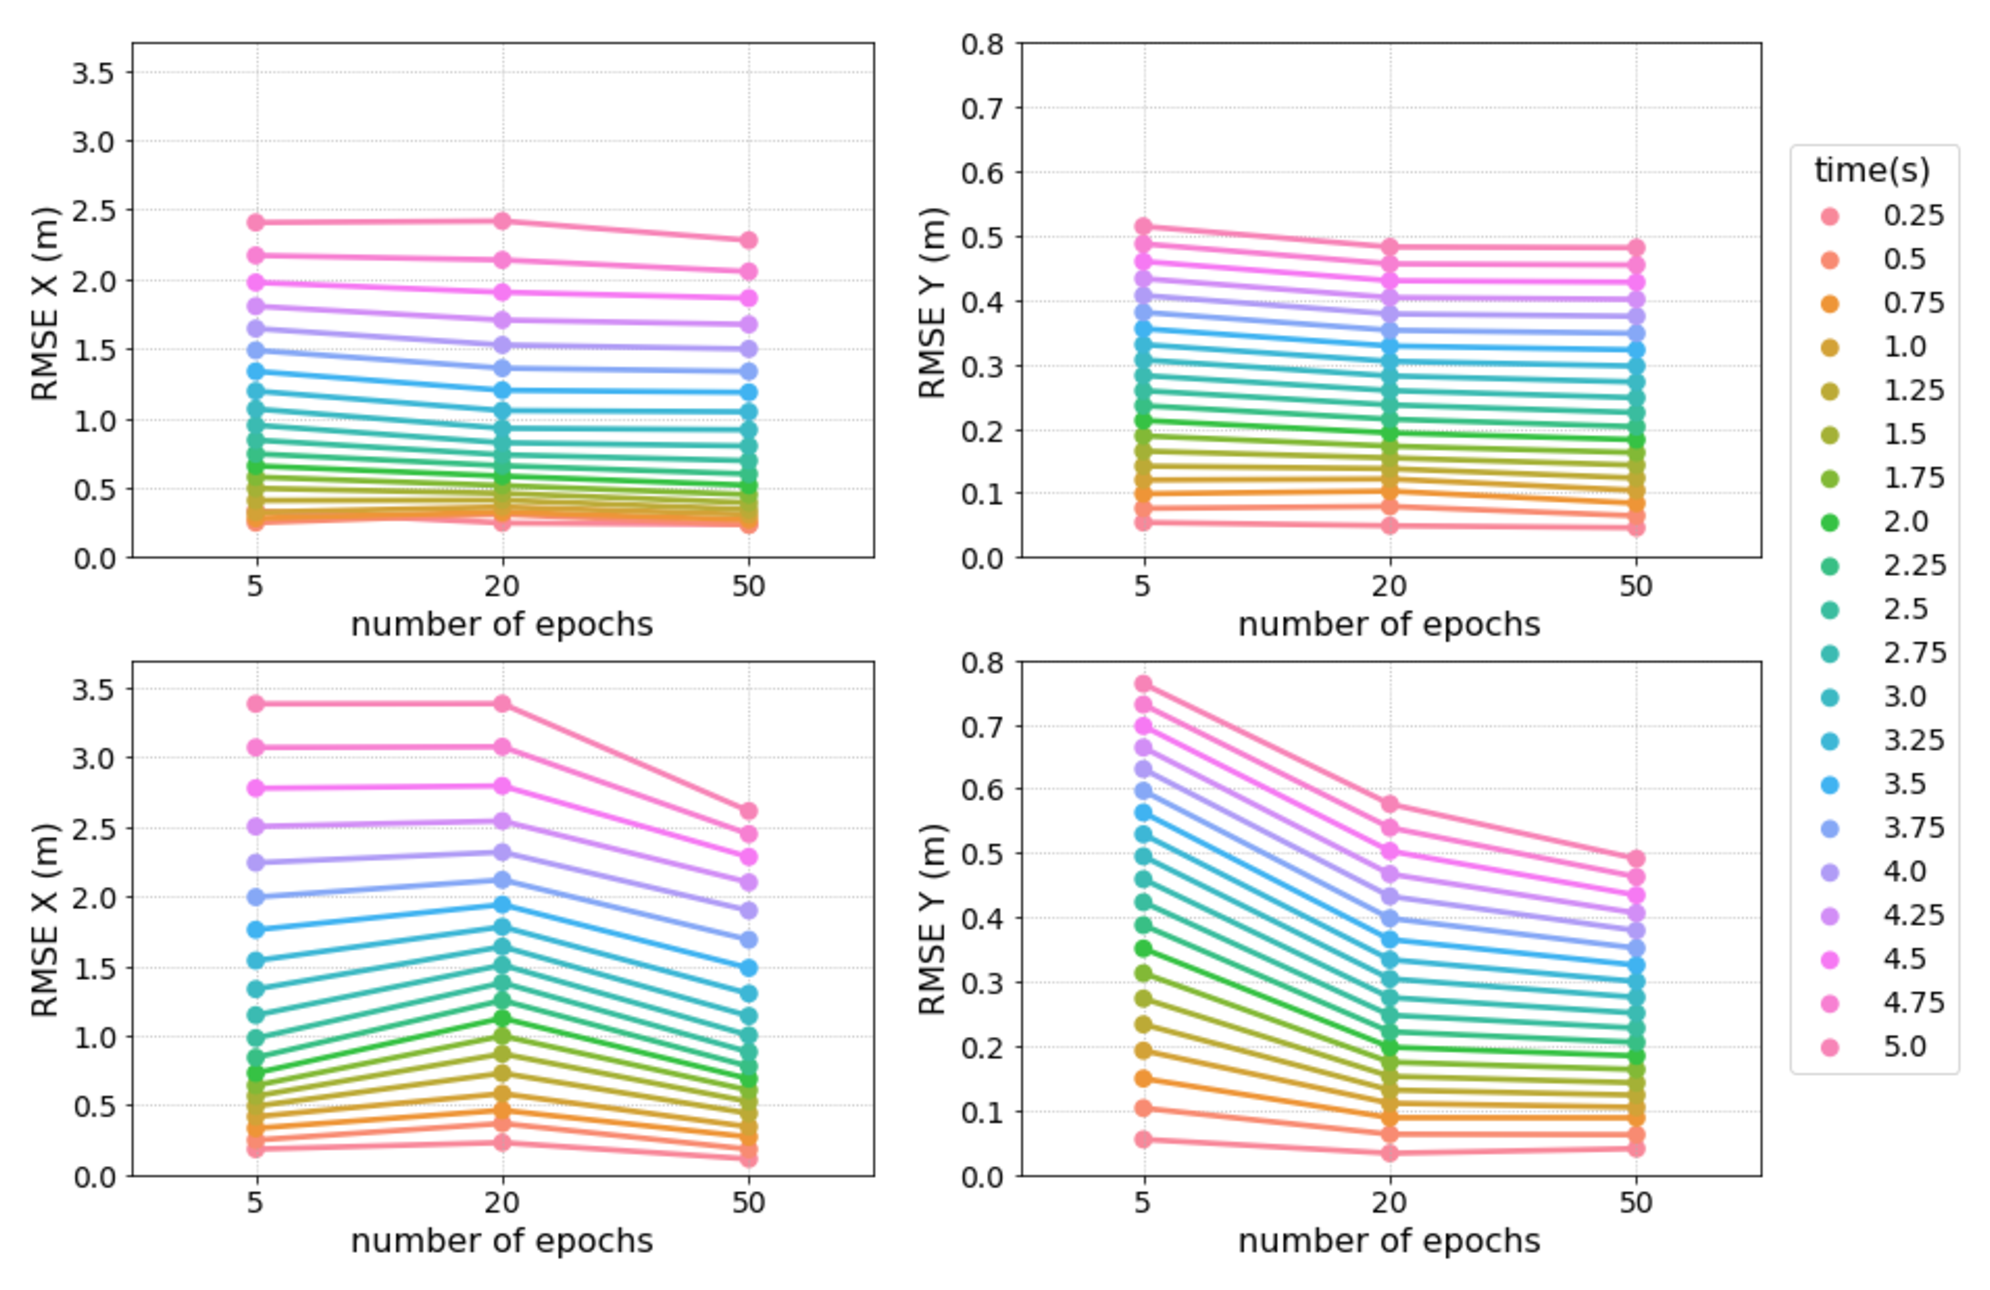
\includegraphics[width=0.9\textwidth]{imgs/lstm_layers_epochs_analysis.eps}
  \caption{Analysis of the \ac{RMSE} varying the number of layers and epochs of our \ac{LSTM} model trained on the \emph{On-board} data set. The left column shows the \ac{RMSE} of a model with only one layer trained for \num{5}, \num{20} and \num{50} epochs, while the right column shows the \ac{RMSE} of a model with \num{10} layers trained for \num{5}, \num{20} and \num{50} epochs.}
  \label{fig:lstm_layers_epochs_analysis}
\end{figure}

We continue our hyperparameter analysis by inspecting the number of dimensions within the \ac{LSTM} cells.
In our initial experiment, we used \num{80} dimensions in each of the \ac{LSTM} encoder and decoder cell.
Here, we investigate if adding more dimensions improves the models' prediction performance.
Again, we train the model for \num{8} epochs.
Figure~\ref{subfig:lstm_units_analysis} depicts the \ac{RMSE} for models with \num{80}, \num{150}, \num{200} and \num{500} dimensions in the \ac{LSTM} cells.
We observe that the model with \num{150} dimensions performs best in $x$-direction whereas all models show comparable performance in $y$-direction.
However, increasing the number of dimensions beyond \num{150} per \ac{LSTM} does not improve the models' accuracy but rather deteriorates the performance.
Therefore, we fix the number of dimensions within the \ac{LSTM} cells to \num{150} for further investigation.

In the next step, we inspect how the number of layers in our network architecture influences the model's performance.
Here, one layer is a pair of one \ac{LSTM} encoder and decoder cell each.
Thus, a model with \num{2} layers consists of a sequence of \num{2} \ac{LSTM} encoder cells followed by a sequence of again \num{2} \ac{LSTM} decoder cells.
Figure~\ref{subfig:lstm_layers_analysis} visualizes the \ac{RMSE} of models with \num{1} up to \num{9} layers trained for \num{8} epochs.
This analysis shows that the model using only one layer performs best and that increasing the number of layers and thus using a deeper network architecture does not improve the model's performance.
On the contrary, more layers lead to worse accuracy in both dimensions.
However, we trained all models for a fixed number of \num{8} epochs whereas deeper network architectures might demand a longer training process.

In the next step, we therefore analyze the number of layers and number of epochs jointly to investigate if larger network architectures trained for more epochs improve prediction performance.
Figure~\ref{fig:lstm_layers_epochs_analysis} visualizes the results of this experiment: the left column depicts the \ac{RMSE} of a model with only one layer trained for \num{5}, \num{20} and \num{50} epochs, whereas the right column shows the \ac{RMSE} of a model with \num{10} layers trained for \num{5}, \num{20} and \num{50} epochs. 
We observe that training a deeper model for more epochs does improve its accuracy.
However, if we compare the left and right plots in Fig.~\ref{fig:lstm_layers_epochs_analysis}, we also find that by training a model with \num{10} layers for \num{50} epochs we only achieve the accuracy of the simpler single-layer \ac{LSTM} model trained for \num{5} epochs.
We conclude, that using more layers even with a longer training process (i.e., increased number of epochs) does not lead to improved prediction results.
Thus, a \ac{LSTM} model with one encoder and decoder cell each is not only the simplest network architecture but also the best in terms of accuracy and time needed for training.

\begin{figure}[t!]
  \centering
  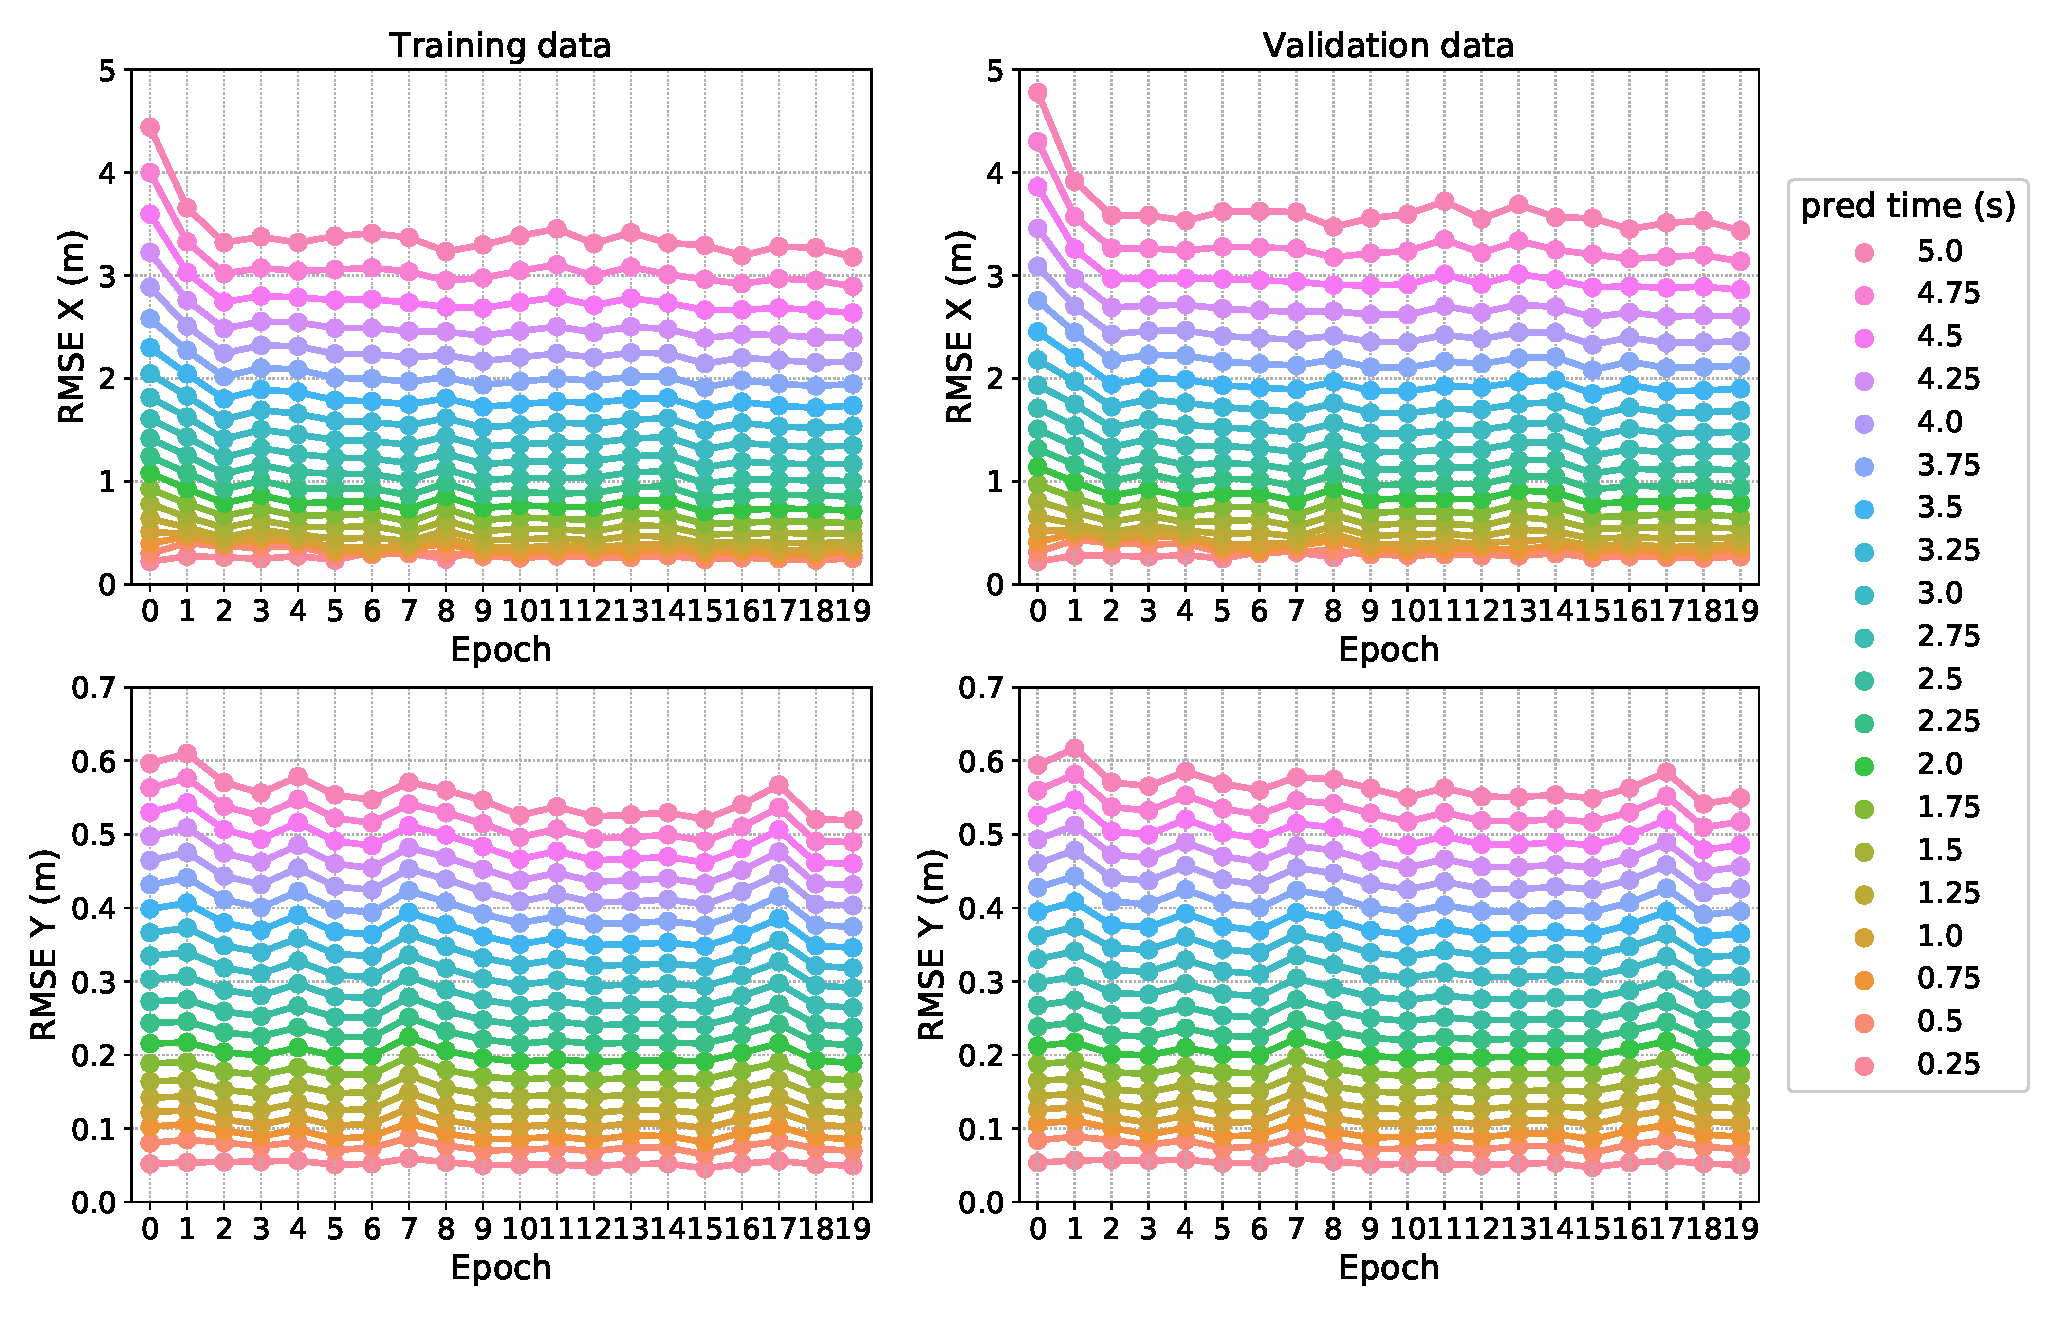
\includegraphics[width=0.95\textwidth]{imgs/rmse_dev_over_epochs.eps}
  \caption{Development of the \ac{RMSE} at every prediction time step during the training process of the \ac{LSTM} \acs{SPA} \num{3} model for each epoch on the training (left column) and validation part (right column) of the \emph{On-board} data set.
  One observes comparable trends on both, training and validation set and that the \ac{RMSE} does not significantly decrease after \num{10} epochs.}\label{fig:rmse_dev_over_epochs}
\end{figure}

We briefly summarize the findings of this section and fix the following set of parameters for subsequent sections: we use a \ac{LSTM} model with one encoder and one decoder cell with \num{150} hidden dimensions each.

\subsubsection{Model training}%
\label{ssubsec:model_training_lstms}

Using the aforementioned network architecture and hyperparameter set, we train one model instantiation for each encoding scheme mentioned in section~\ref{subsec:scene_representation_in_vectors}, whereas only the input dimensionality of the encoder cell changes when varying the representation of the input data.
Importantly, we focus on positional information as the only input for our \ac{LSTM} models in this work for reasons of consistency to make all models as comparable as possible.
Hence, we neglect for example the history of the target (or ego-) vehicle's velocity or acceleration as input here.
Between the two data sets, the only difference between models is the auxiliary data, that is used as additional input to the \ac{LSTM} decoder cell at each time step.
For both data sets, we use the instantaneous velocity of the target vehicle to aid the model predicting the future trajectory at every time step.
As there is no ego-vehicle present in the \emph{\ac{NGSIM}} data set $D_2$, we use no further auxiliary data.
For the \emph{On-board} data set $D_1$, we use the ego-vehicle's predicted acceleration and the estimated curvature of the ego-vehicle's current lane.
Although this is future information, we argue that it is solely about the ego-vehicle, which we expect to be available at the time the prediction is to happen.
We assume, that an automated vehicle, in order to safely navigate, will have an estimation of the future lane curvature as well as the acceleration values of its own planned trajectory.
Furthermore, we employed early stopping, that is, we trained our models for \num{10} epochs as we found that the models' performance stagnate on both, training and validation data sets, when training for up until a total \num{20} epochs.
Figure~\ref{fig:rmse_dev_over_epochs} visualizes this result by showing the development of the \ac{RMSE} of the \ac{LSTM} \acs{SPA} \num{3} model using the \ac{SPA}-power-with-ego vector representation $(\mathbf{S}_{t}^{ego})_{t_0}^{t_N}$ as input for the training (Fig.~\ref{fig:rmse_dev_over_epochs} left column) and validation part (Fig.~\ref{fig:rmse_dev_over_epochs} right column) of the \emph{On-board} data set $D_1$.
On the $y$-axis of each sub-figure, we have the \ac{RMSE} while the $x$-axis from left to right depicts the result after each epoch during the training process.
Each colored line illustrates the \ac{RMSE} of the model for one particular prediction time step while all points with the same value on the $x$-axis depict the model's performance after the respective epoch during the training process.

\subsubsection{Evaluation}%
\label{ssubsec:evaluation_lstms}

\begin{figure}[t!]
	\centering
    \subfloat[\label{subfig:lstm_rmse_all_on_board}]{%
        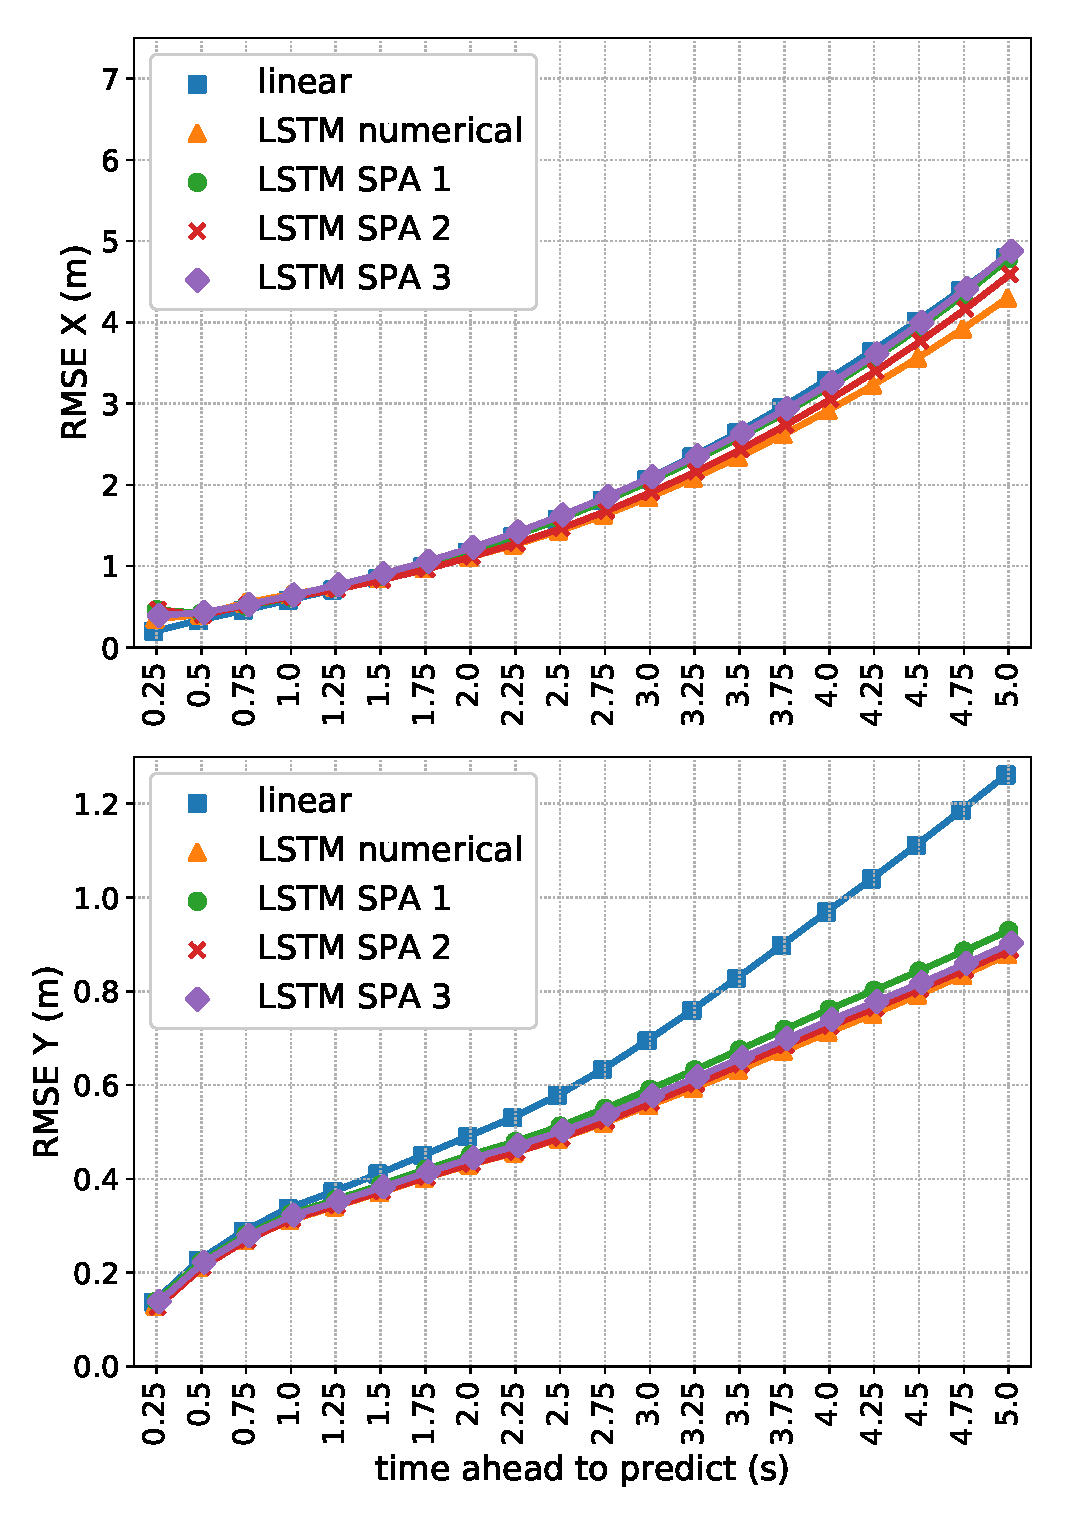
\includegraphics[width=0.5\columnwidth]{imgs/rmse_large_all.eps}
    }
    %\vspace{-0.3cm}
    \subfloat[\label{subfig:lstm_rmse_subset_on_board}]{%
        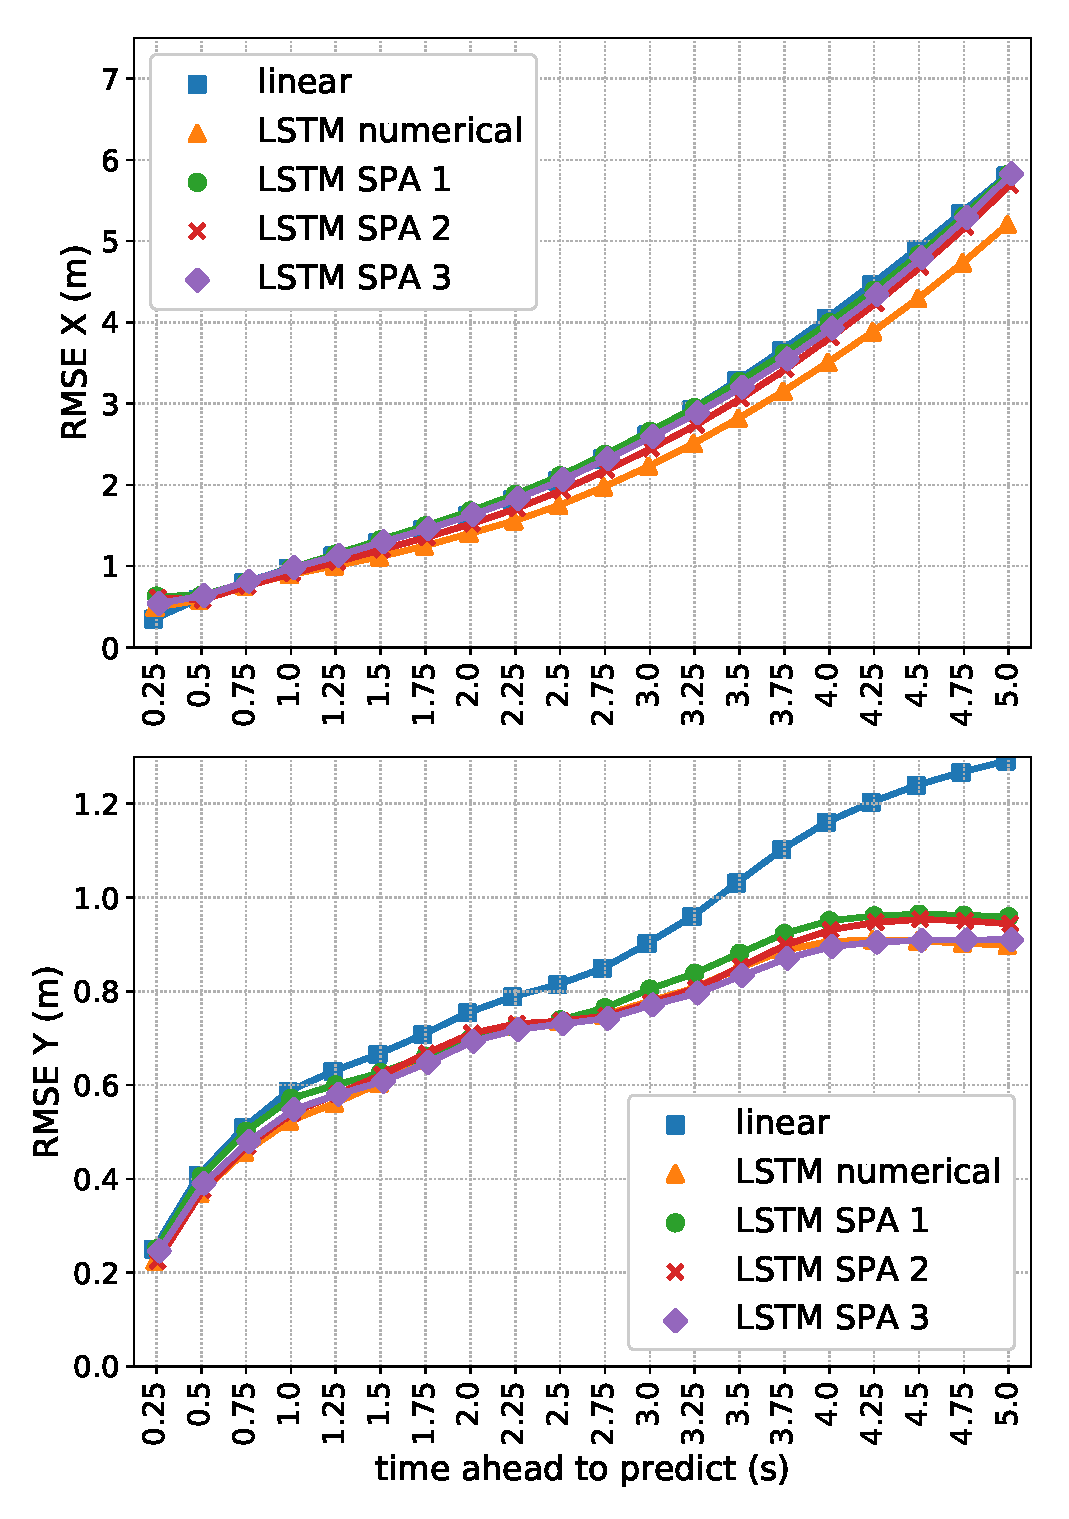
\includegraphics[width=0.5\columnwidth]{imgs/rmse_large_subset.eps}
    }
    \caption{Visualization of the \ac{RMSE} of all \ac{LSTM} models on the \emph{On-board} data set:~\protect\subref{subfig:lstm_rmse_all_on_board} shows the complete validation set $V_1 \subset D_1$~\protect\subref{subfig:lstm_rmse_subset_on_board} shows the subset of situations with at least \num{3} other vehicles present and distance between the target and ego-vehicle lower than  \SI{20}{\meter} and between target and closest other vehicle lower than \SI{10}{\meter}.}\label{fig:rmse_on_board_all}
\end{figure}

Figure~\ref{fig:rmse_on_board_all} visualizes the \ac{RMSE} of all \ac{LSTM}-based models on the validation-set $V_1 \subset D_1$ of the \emph{On-board} data set using \num{512}-dimensional vectors.
Figure~\ref{subfig:lstm_rmse_all_on_board} shows the performance on the complete validation-set, whereas Fig.~\ref{subfig:lstm_rmse_subset_on_board} depicts only situations with at least \num{3} other vehicles present, the distance between the target and the ego-vehicle being lower than \SI{20}{\meter} and the distance between the target and the closest other vehicle being less than \SI{10}{\meter}.
We observe that all approaches yield comparable results with notable differences in certain situations.
Although the models employing the \ac{SPA}-power encoding schemes tend to perform worst in $x$-direction, we observe that they perform better in $y$-direction in crowded situations with closely driving vehicles with the \acs{LSTM} \acs{SPA} \num{3} model ranking best along the \acs{LSTM} numerical model.
\begin{figure}[t!]
    \centering
    \subfloat[\label{subfig:histogram_on_board_1}]{%
        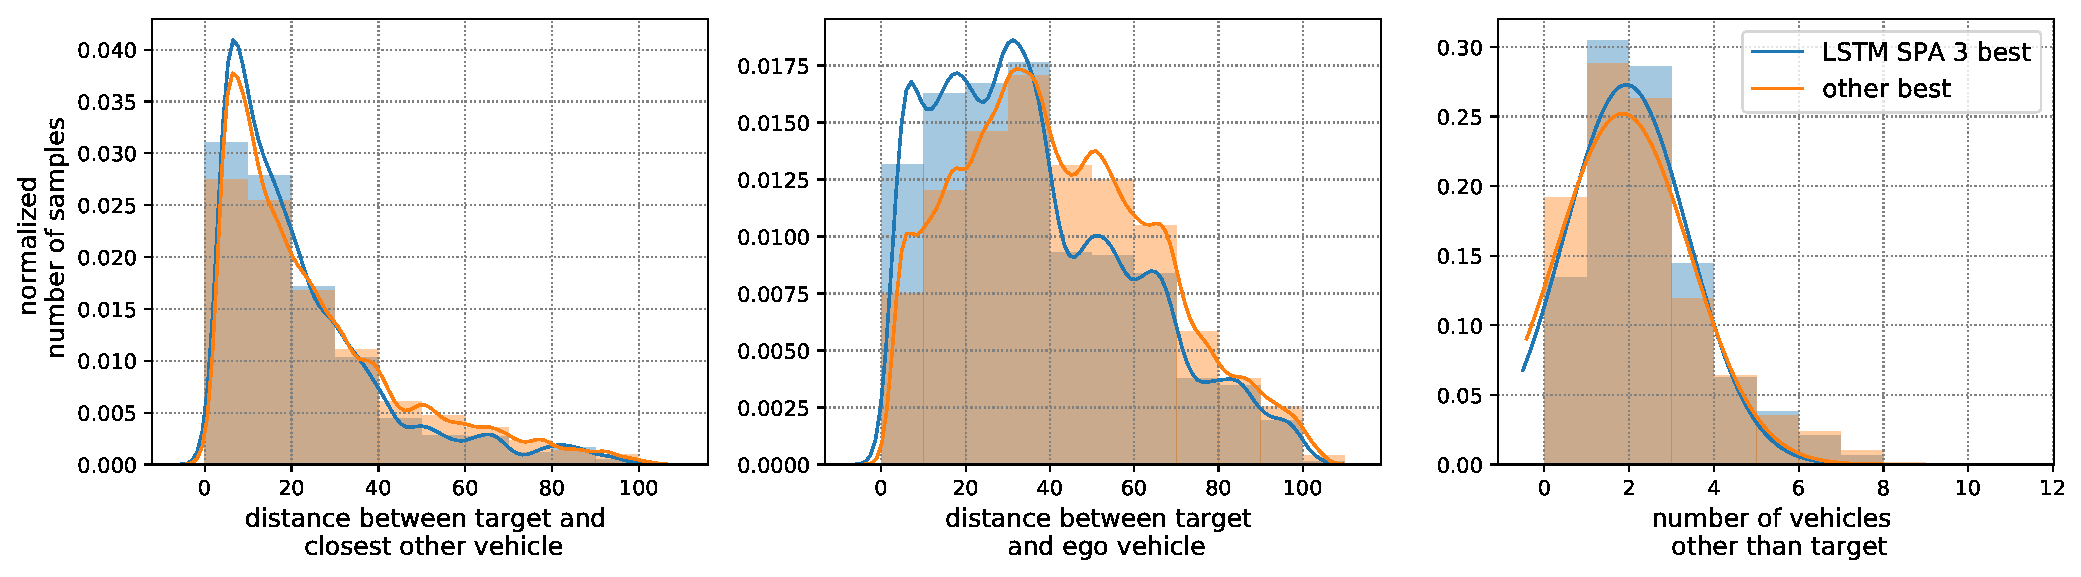
\includegraphics[width=0.95\linewidth]{imgs/histogram_on_board_1.eps}
    }\\
    \subfloat[\label{subfig:histogram_on_board_2}]{%
        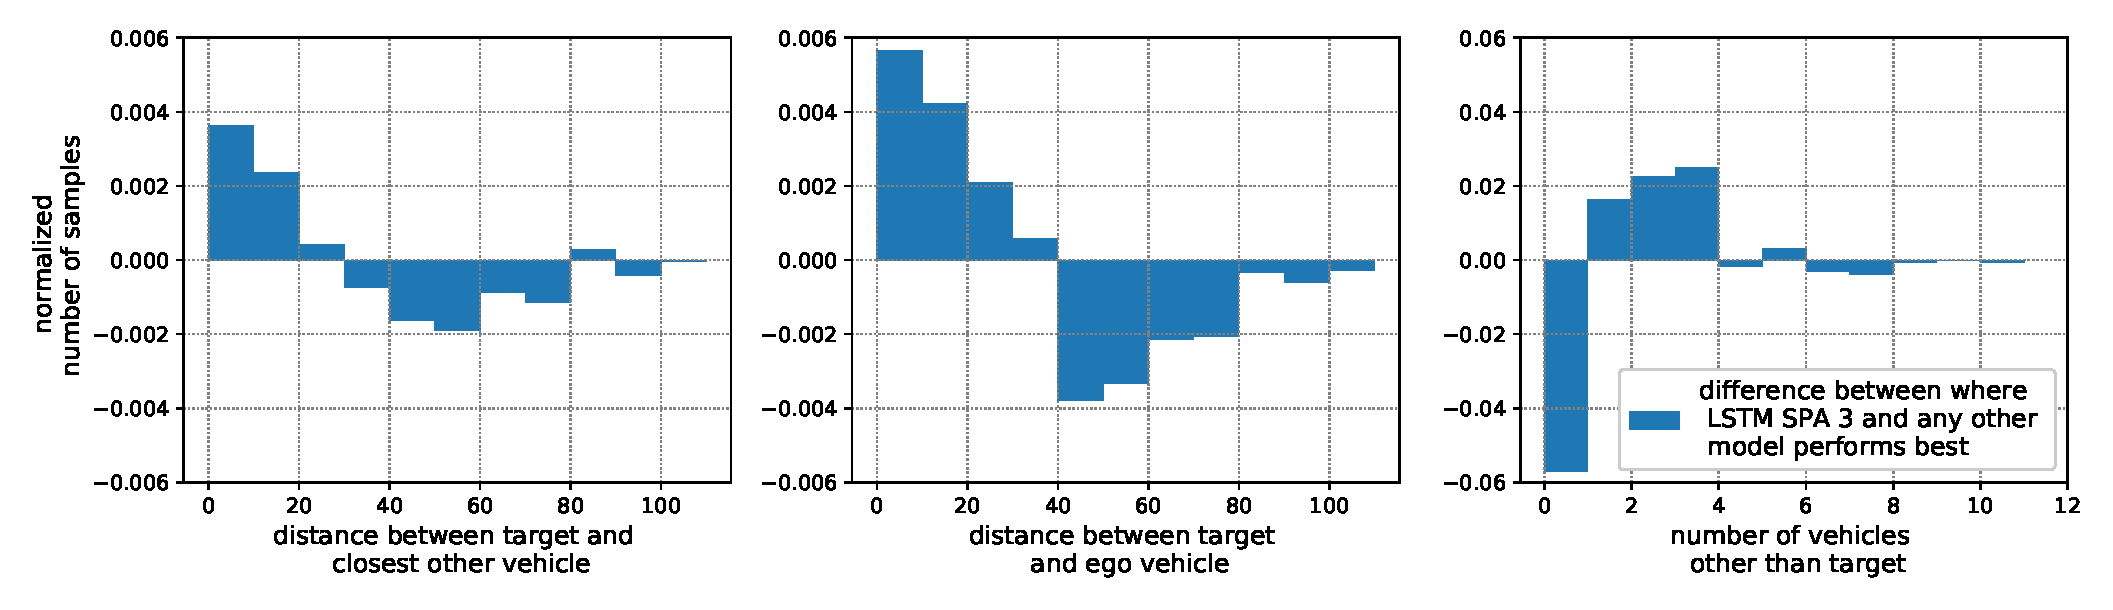
\includegraphics[width=0.95\linewidth]{imgs/histogram_on_board_2.eps}
    }
    \caption{Metric evaluation specifying situations where the \ac{LSTM} \acs{SPA} \num{3} model outperforms all other approaches regarding the \acs{RMSE} in $y$-direction on the \emph{On-board} data set $D_1$.
      In the upper row~\protect\subref{subfig:histogram_on_board_1}, blue bars illustrate samples where \ac{LSTM} \ac{SPA} \num{3} performs better than all other models while the orange bars depict samples where any other model performs best.
      From left to right, the plots in ~\protect\subref{subfig:histogram_on_board_1} illustrate the distance between the target vehicle and the closest other vehicle, the distance between the target and the ego-vehicle and the number of vehicles other than the target.
      The lower row~\protect\subref{subfig:histogram_on_board_2} illustrates the difference between the blue and orange bars in the corresponding plot in~\protect\subref{subfig:histogram_on_board_1}.
    }
    \label{fig:histograms_on_board}
\end{figure}

To further investigate this result, we evaluated certain metrics, chosen to characterize crowded and potentially dangerous situations, for items in the validation set, where the \ac{LSTM} \ac{SPA} \num{3} model outperforms all other approaches with respect to the \ac{RMSE} in $y$-direction (see Fig.~\ref{fig:histograms_on_board}).
We observe that the number of samples, where the distance between the target and the ego-vehicle and/or the closest other object being small is significantly higher when the \ac{LSTM} \ac{SPA} \num{3} model outperforms all other approaches.
For samples where the \ac{LSTM} \ac{SPA} \num{3} model performs best, the number of samples with a distance less than \SI{20}{\meter} between the target and ego-vehicle is \SI{50.5}{\percent} higher compared to samples where any of the other models performs best.
For distances less than \SI{20}{\meter} between the target vehicle and the closest other vehicle, the number of samples is still \SI{11.4}{\percent} higher when the \ac{LSTM} \ac{SPA} \num{3} model performs best.
Finally, the number of situations with at least \num{3} other vehicles present is also \SI{7.8}{\percent} higher compared to samples where any other model performs best.
However, we aim to investigate more sophisticated options such as clustering methods in future work to uncover other, potentially more meaningful features compared to the ones shown in this paper, distinguishing between situations where \ac{LSTM} \ac{SPA} \num{3} performs best compared to another model showing the best performance.

\begin{figure}[t!]
	\centering
    \subfloat[\label{subfig:lstm_rmse_512_ngsim}]{%
        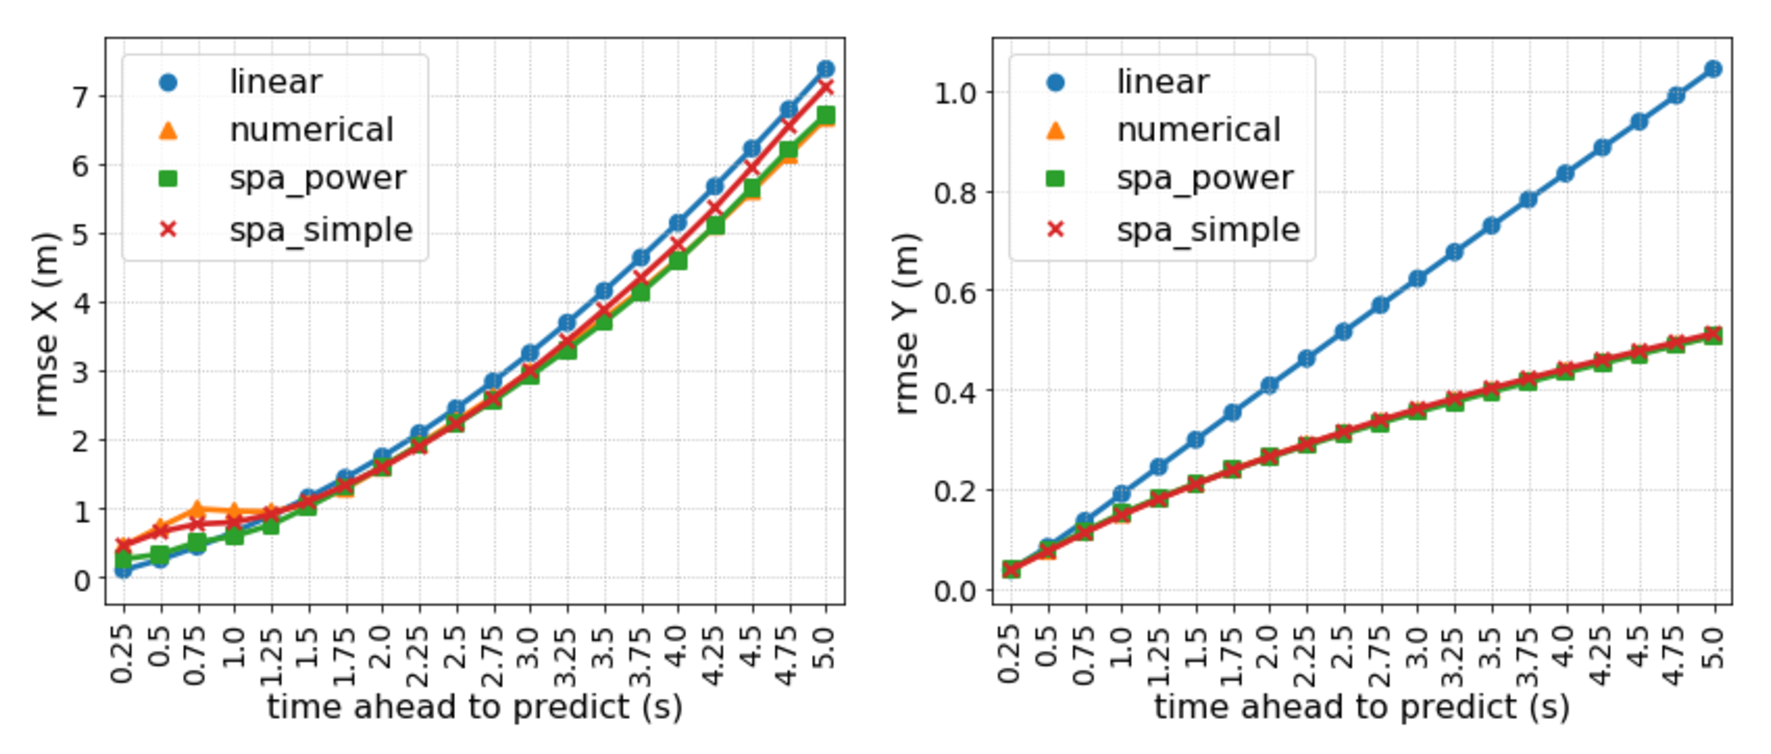
\includegraphics[width=0.5\columnwidth]{imgs/rmse_ngsim_512_10epochs.eps}
    }
    \subfloat[\label{subfig:lstm_rmse_1024_ngsim}]{%
        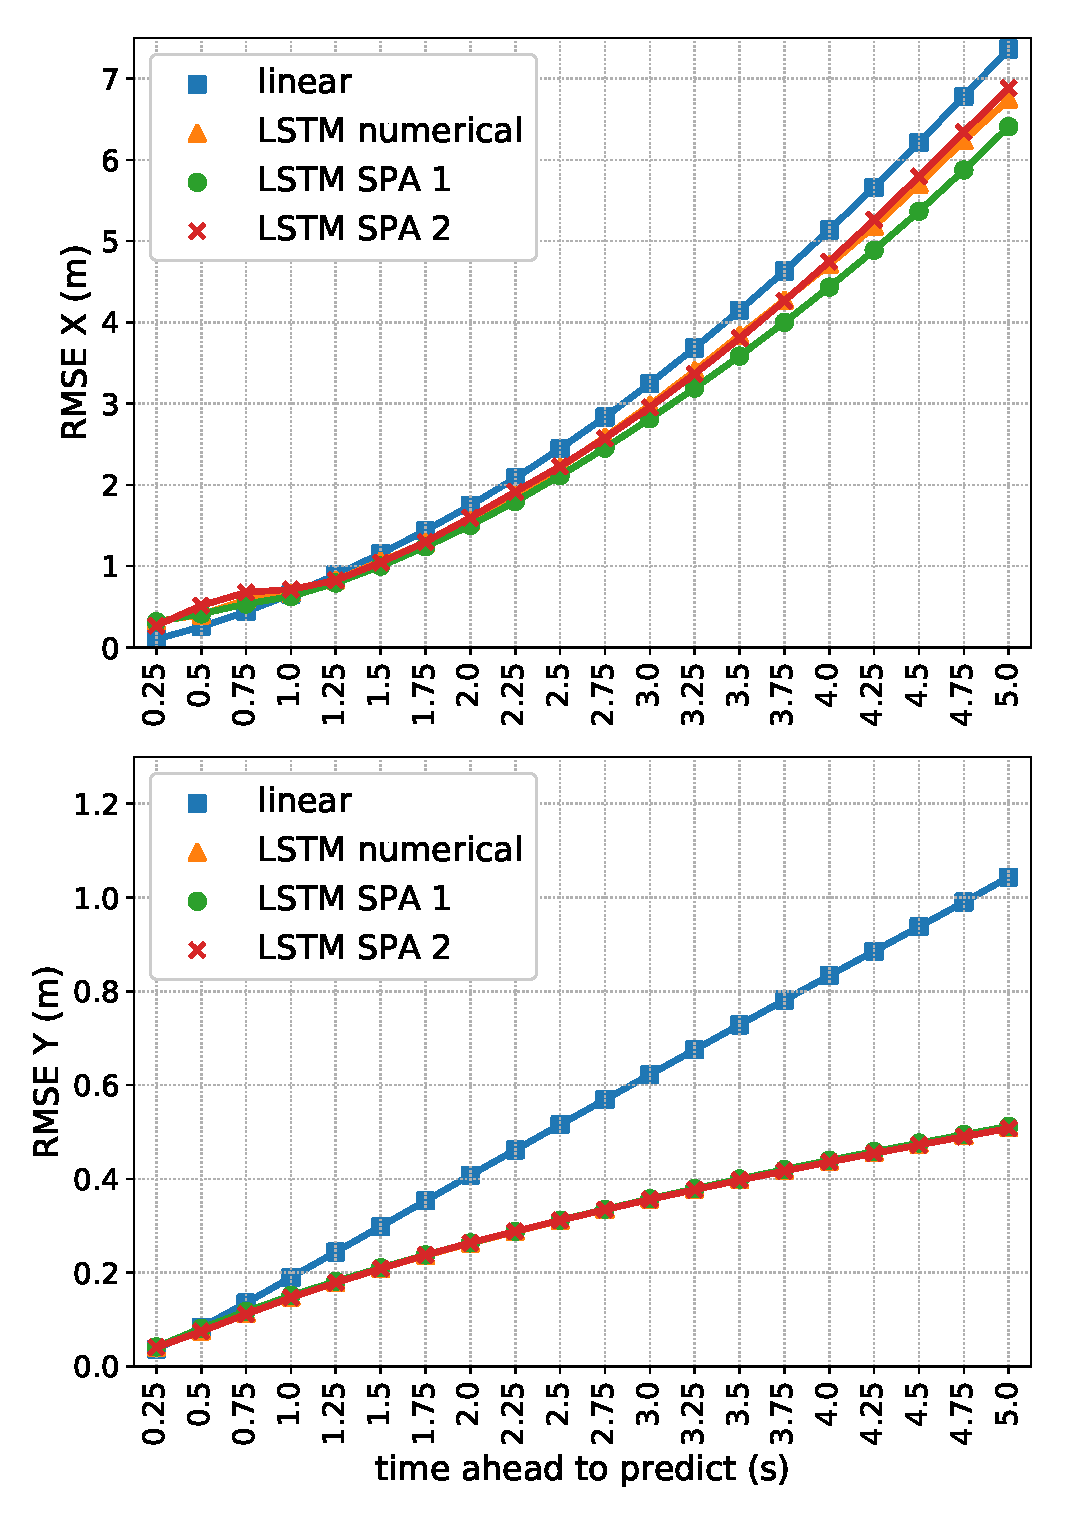
\includegraphics[width=0.5\columnwidth]{imgs/rmse_ngsim_1024_10epochs.eps}
    }

    \caption{Visualization of the \ac{RMSE} of all \ac{LSTM} models on the \emph{\ac{NGSIM}} validation set $V_2 \subset D_2$ using~\protect\subref{subfig:lstm_rmse_512_ngsim} vectors of dimension $512$ for the \ac{SPA}-based models and~\protect\subref{subfig:lstm_rmse_1024_ngsim} using vectors of dimension $1024$ for the \ac{SPA}-based models.}\label{fig:rmse_ngsim_all}

\end{figure}

Figure~\ref{fig:rmse_ngsim_all} visualizes the \ac{RMSE} of all \ac{LSTM}-based models on the validation-set $V_2 \subset D_2$ of the \emph{\ac{NGSIM}} data set for \num{512}-dimensional vectors (Fig.~\ref{subfig:lstm_rmse_512_ngsim}) and for \num{1024}-dimensional vectors (Fig.~\ref{subfig:lstm_rmse_1024_ngsim}).
We observe, that all \ac{LSTM} models achieve a very similar performance (almost identical in $y$-direction) with \ac{LSTM} \ac{SPA} \num{1} achieving the best performance in $x$-direction being on par with the numerical encoding for \num{512}-dimensional vectors.
For \num{1024}-dimensional vectors, \ac{LSTM} \ac{SPA} \num{1} even slightly outperforms all other approaches in $x$-direction, whereas we do not observe significant improvements in $y$-direction.

\paragraph{Evaluation of models trained on data set variations}%
\label{par:evaluation_of_models_trained_on_data_set_variations}

\begin{figure}[th!]
    \centering
    \subfloat[\label{subfig:rmse_large_all}Trained and evaluated on complete data set]{%
        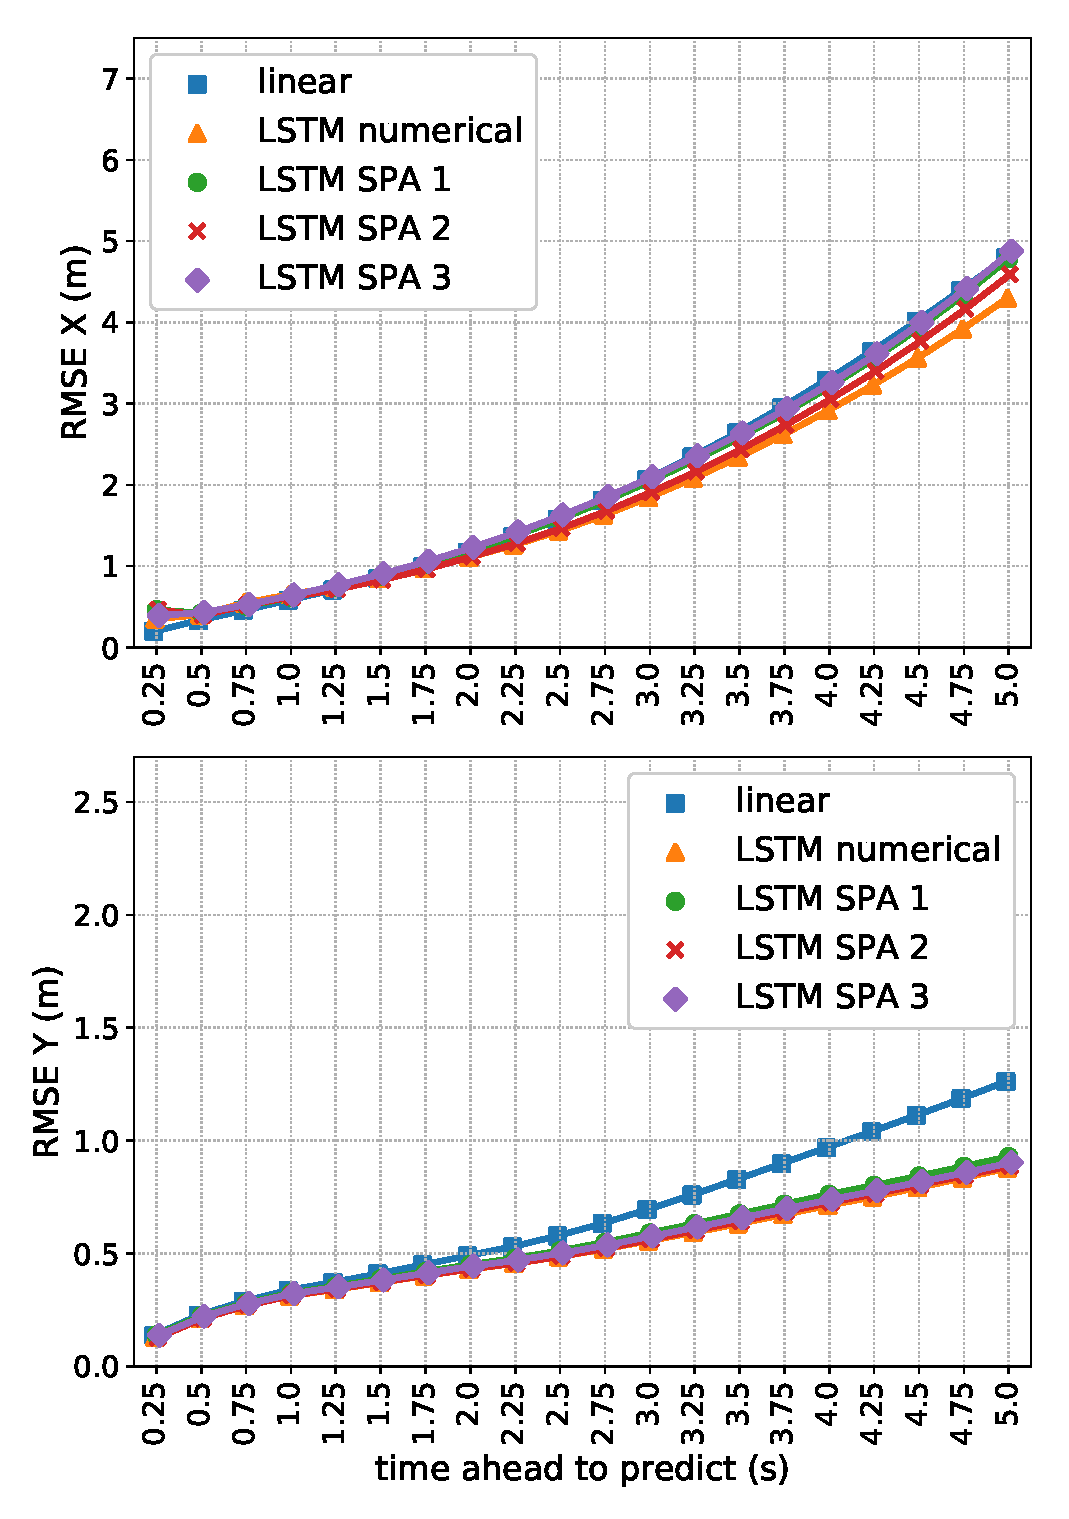
\includegraphics[width=0.25\linewidth]{imgs/rmse_large_all_trained_on_all.eps}
    }
    \subfloat[\label{subfig:rmse_large_all_trained_on_lc}Trained on lane change samples, evaluated on complete data set]{%
        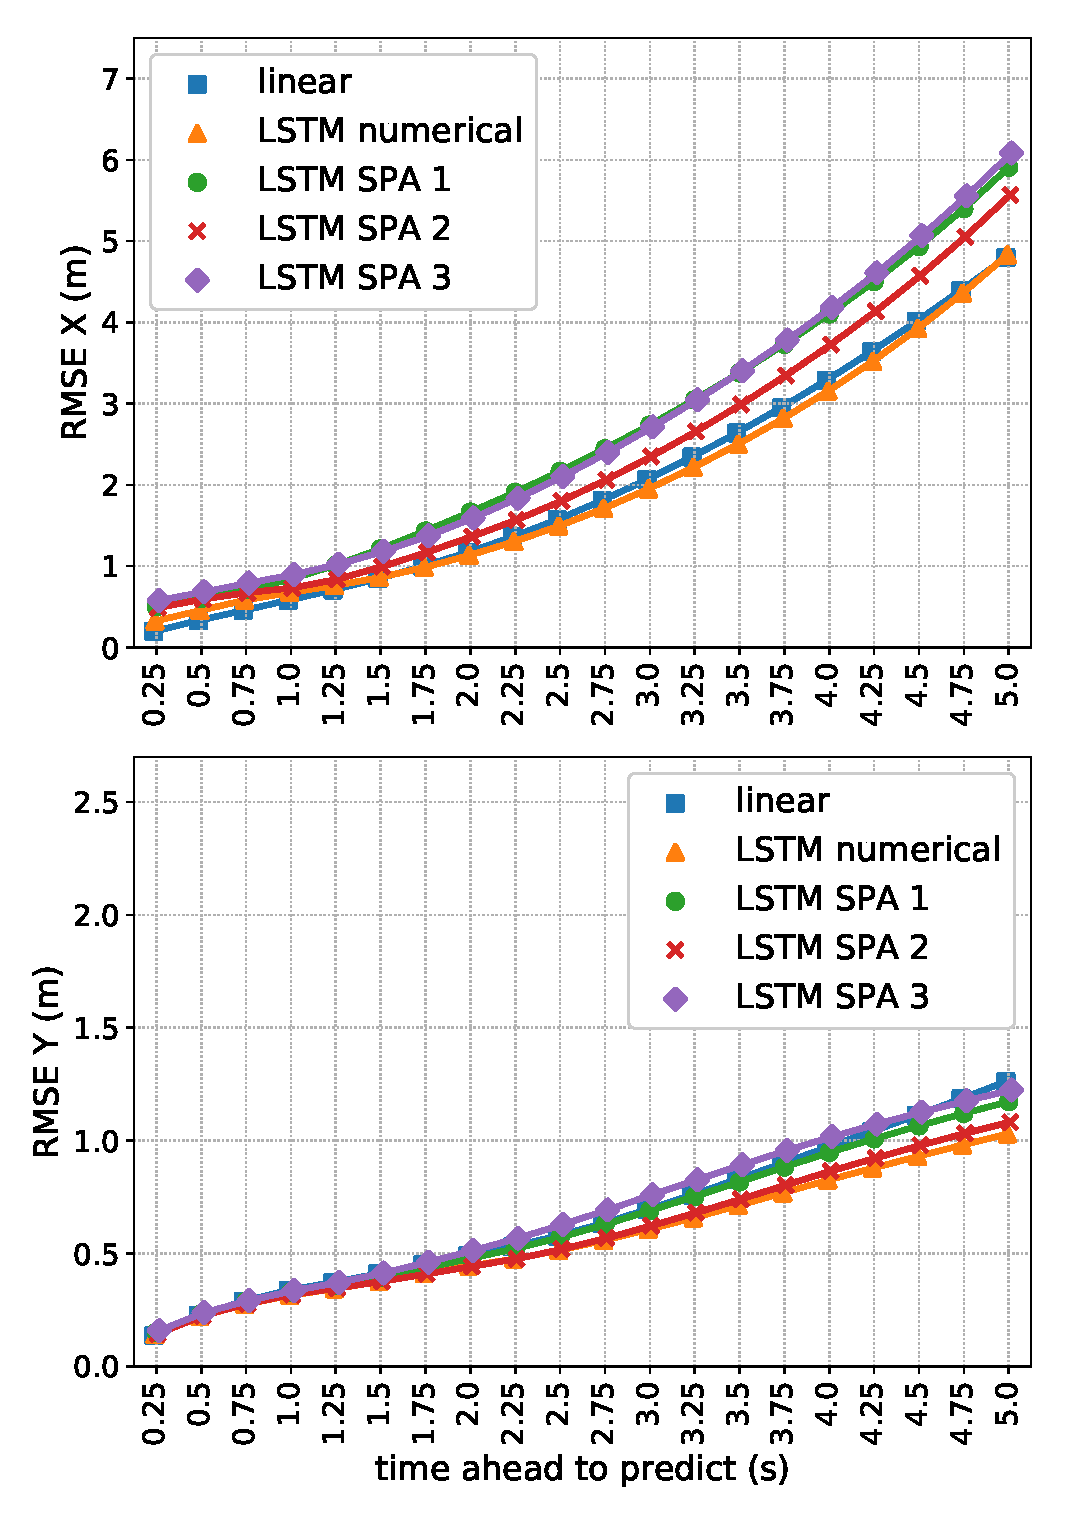
\includegraphics[width=0.25\linewidth]{imgs/rmse_large_all_trained_on_lc.eps}
    }
    \subfloat[\label{subfig:rmse_large_all_lc_only}Trained on complete data set, evaluated on lane changes samples]{%
        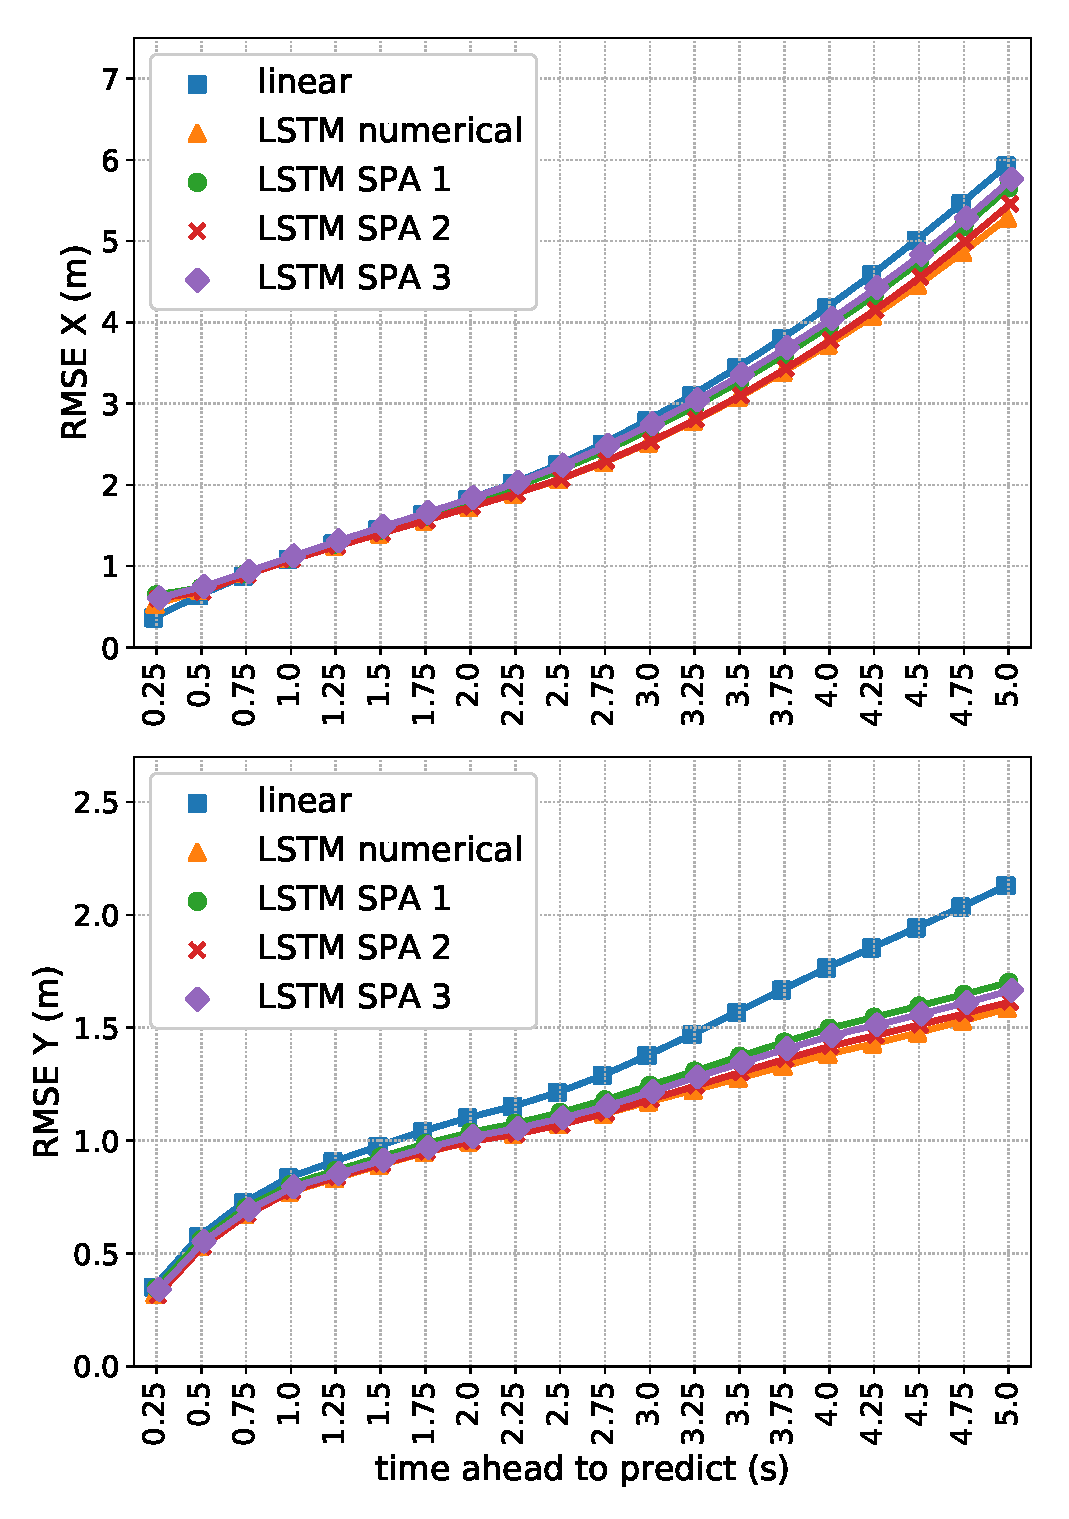
\includegraphics[width=0.25\linewidth]{imgs/rmse_large_all_trained_on_all_evaluated_on_lc.eps}
    }
    \subfloat[\label{subfig:rmse_large_all_lc_only_trained_on_lc}Trained and evaluated on lane change samples ]{%
        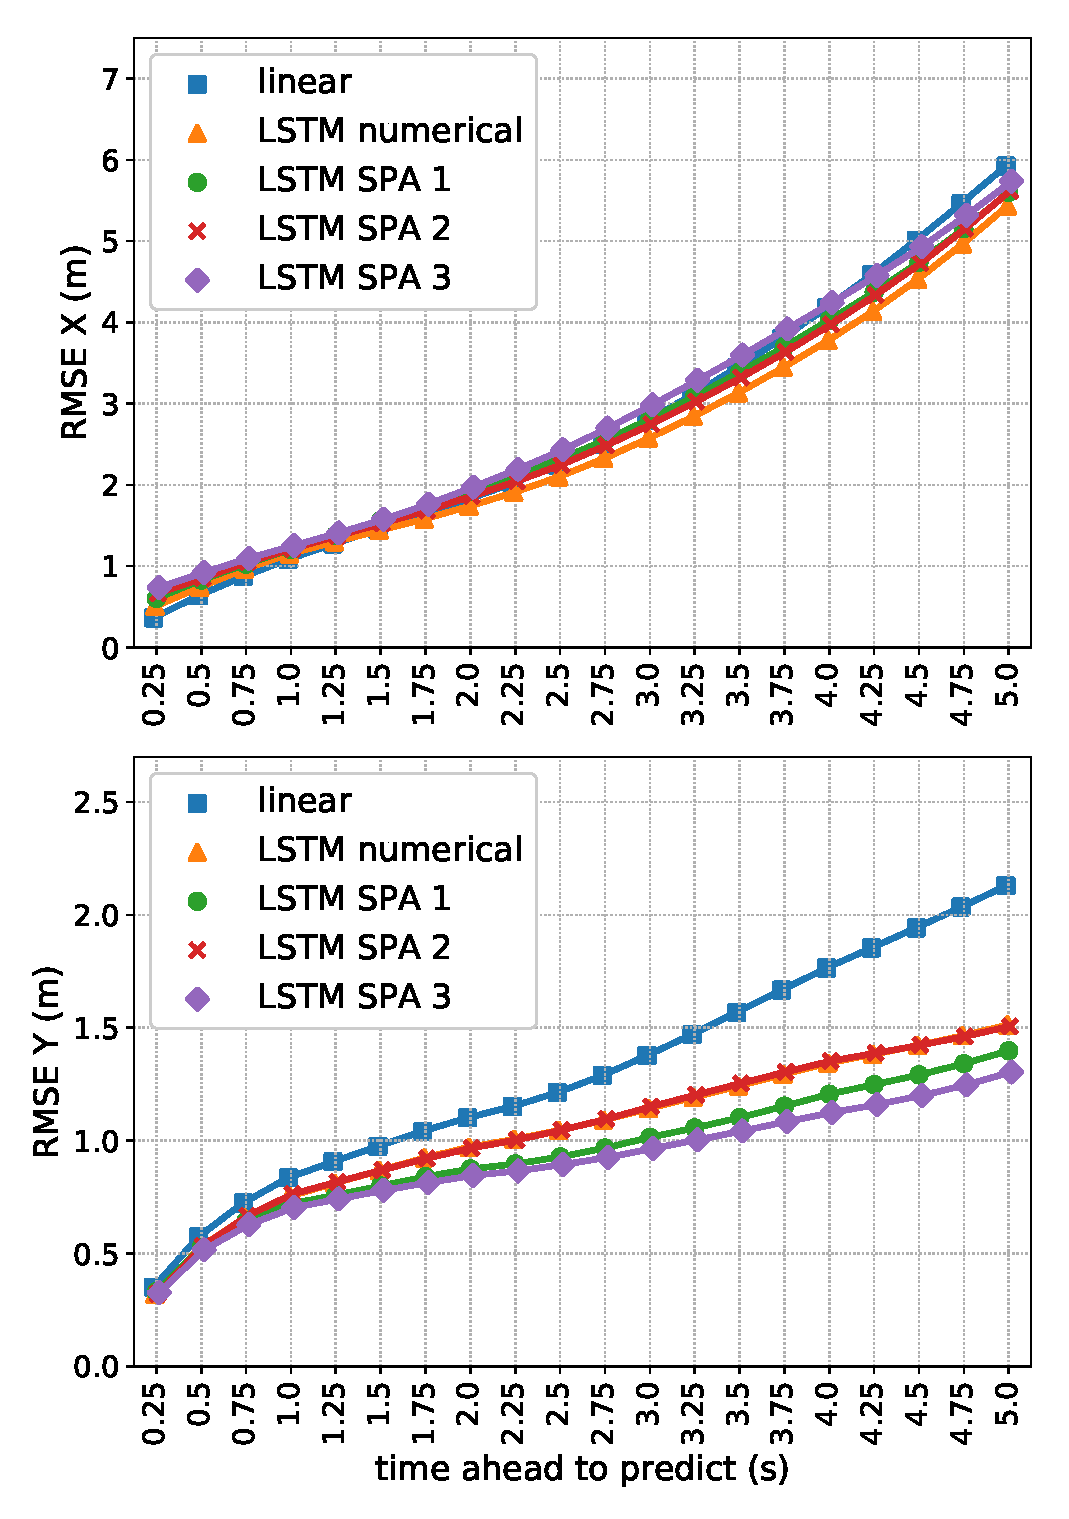
\includegraphics[width=0.25\linewidth]{imgs/rmse_large_all_trained_on_lc_evaluated_on_lc.eps}
    }\\
    \subfloat[\label{subfig:rmse_large_subset}Trained on complete data set, evaluated on crowded situations]{%
        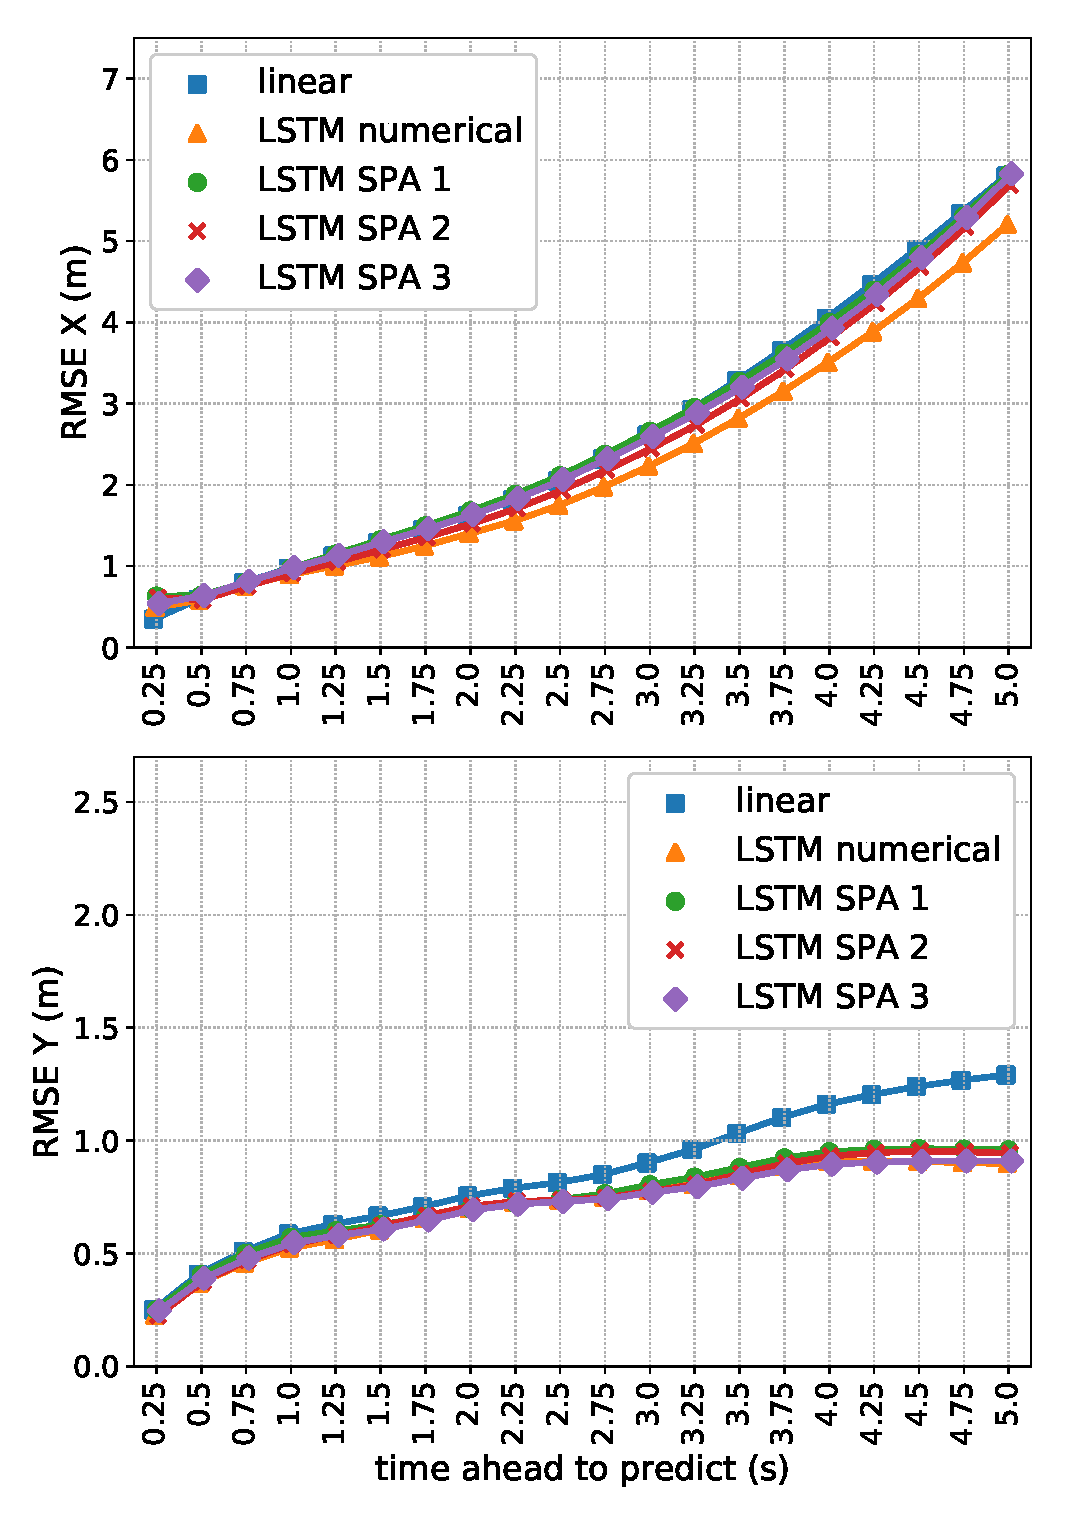
\includegraphics[width=0.25\linewidth]{imgs/rmse_large_subset_trained_on_all.eps}
    }
    \subfloat[\label{subfig:rmse_large_subset_trained_on_lc}Trained on lane change samples, evaluated on crowded situations]{%
        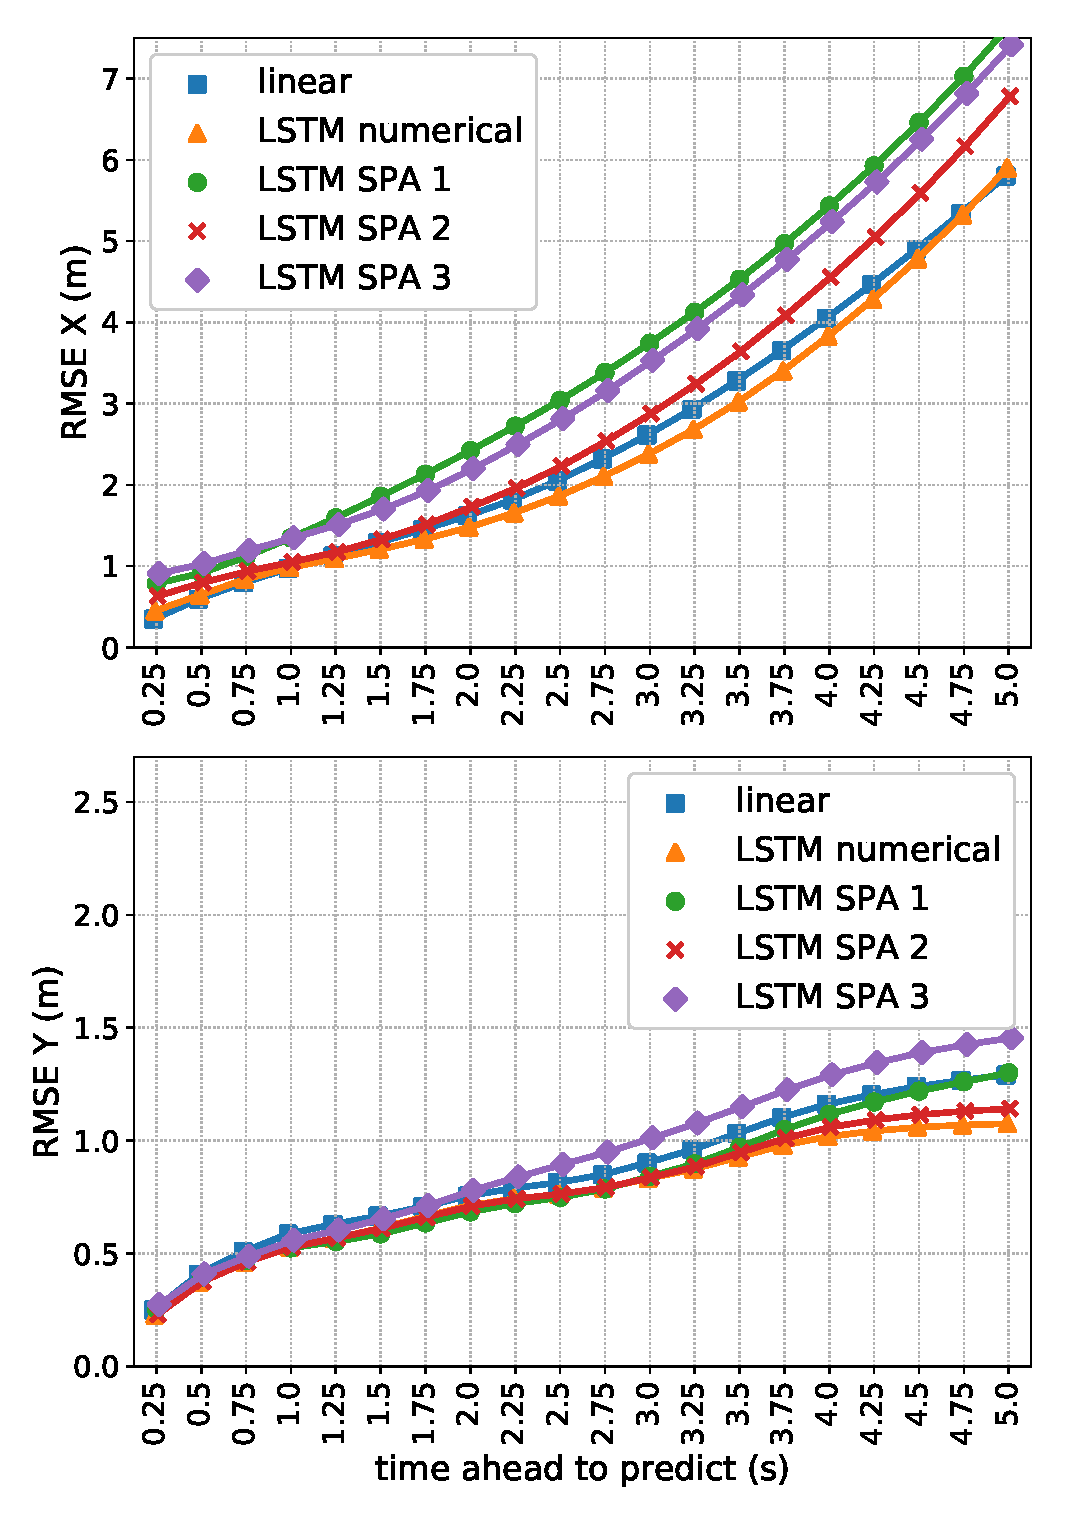
\includegraphics[width=0.25\linewidth]{imgs/rmse_large_subset_trained_on_lc.eps}
    }
    \subfloat[\label{subfig:rmse_large_subset_lc_only}Trained on complete data set, evaluated on crowded situations with lane changes]{%
        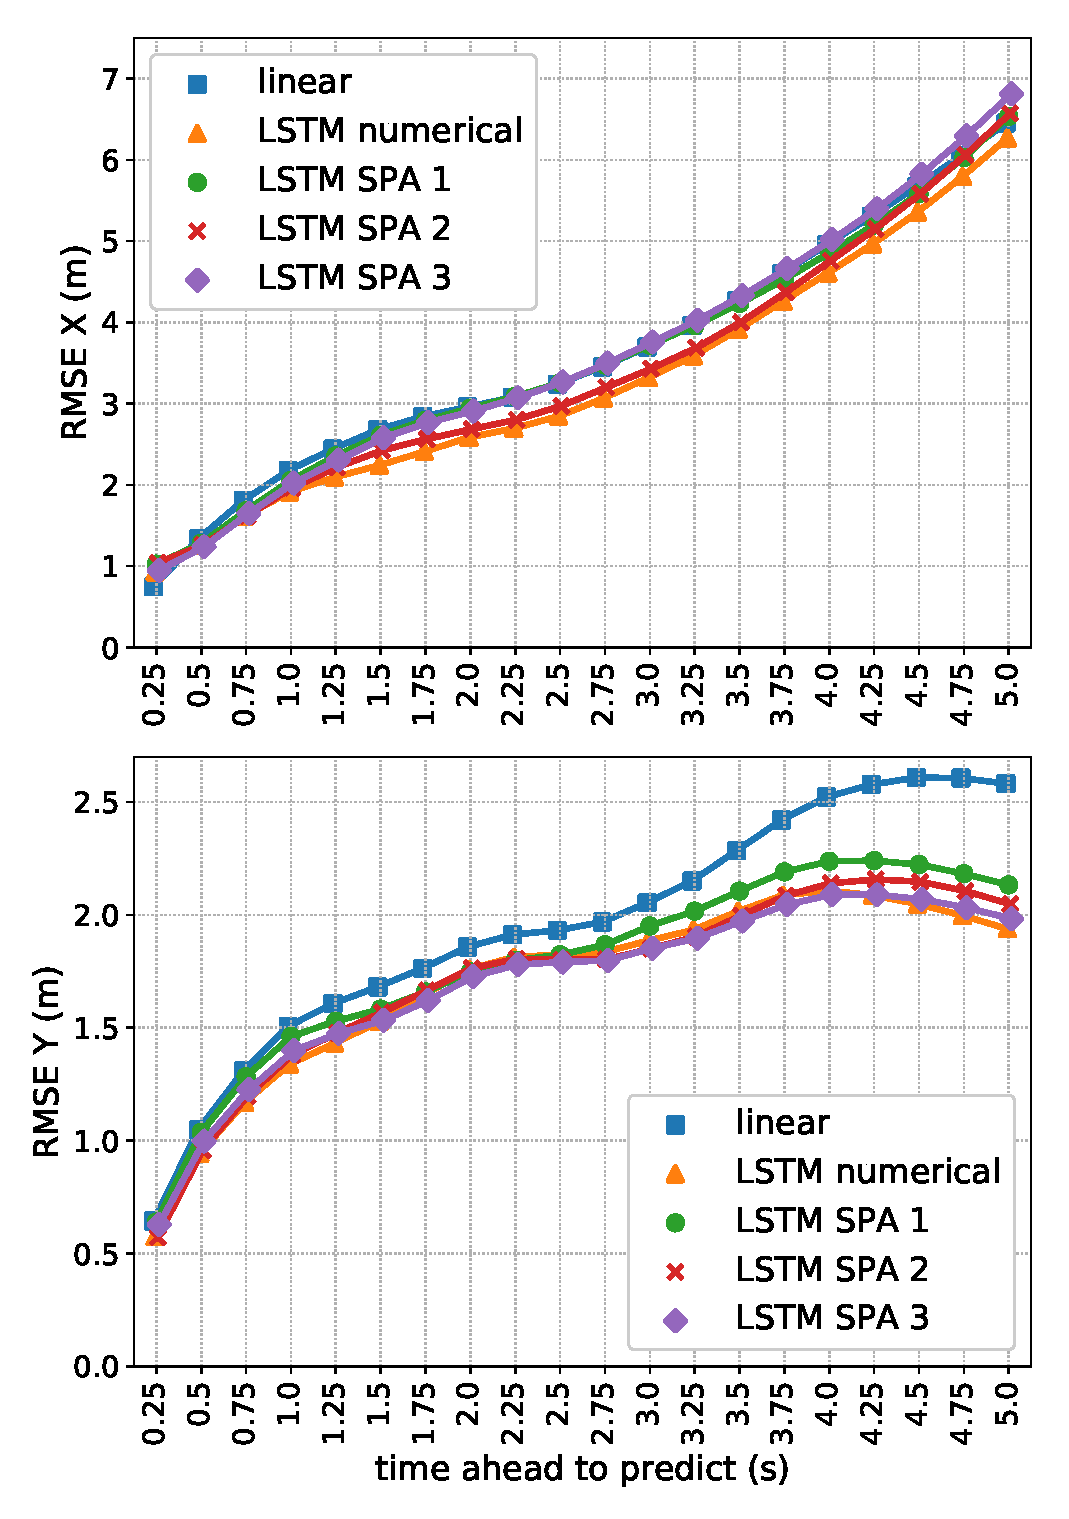
\includegraphics[width=0.25\linewidth]{imgs/rmse_large_subset_trained_on_all_evaluated_on_lc.eps}
    }
    \subfloat[\label{subfig:rmse_large_subset_lc_only_trained_on_lc}Trained on lane change samples, evaluated on crowded situations with lane changes]{%
        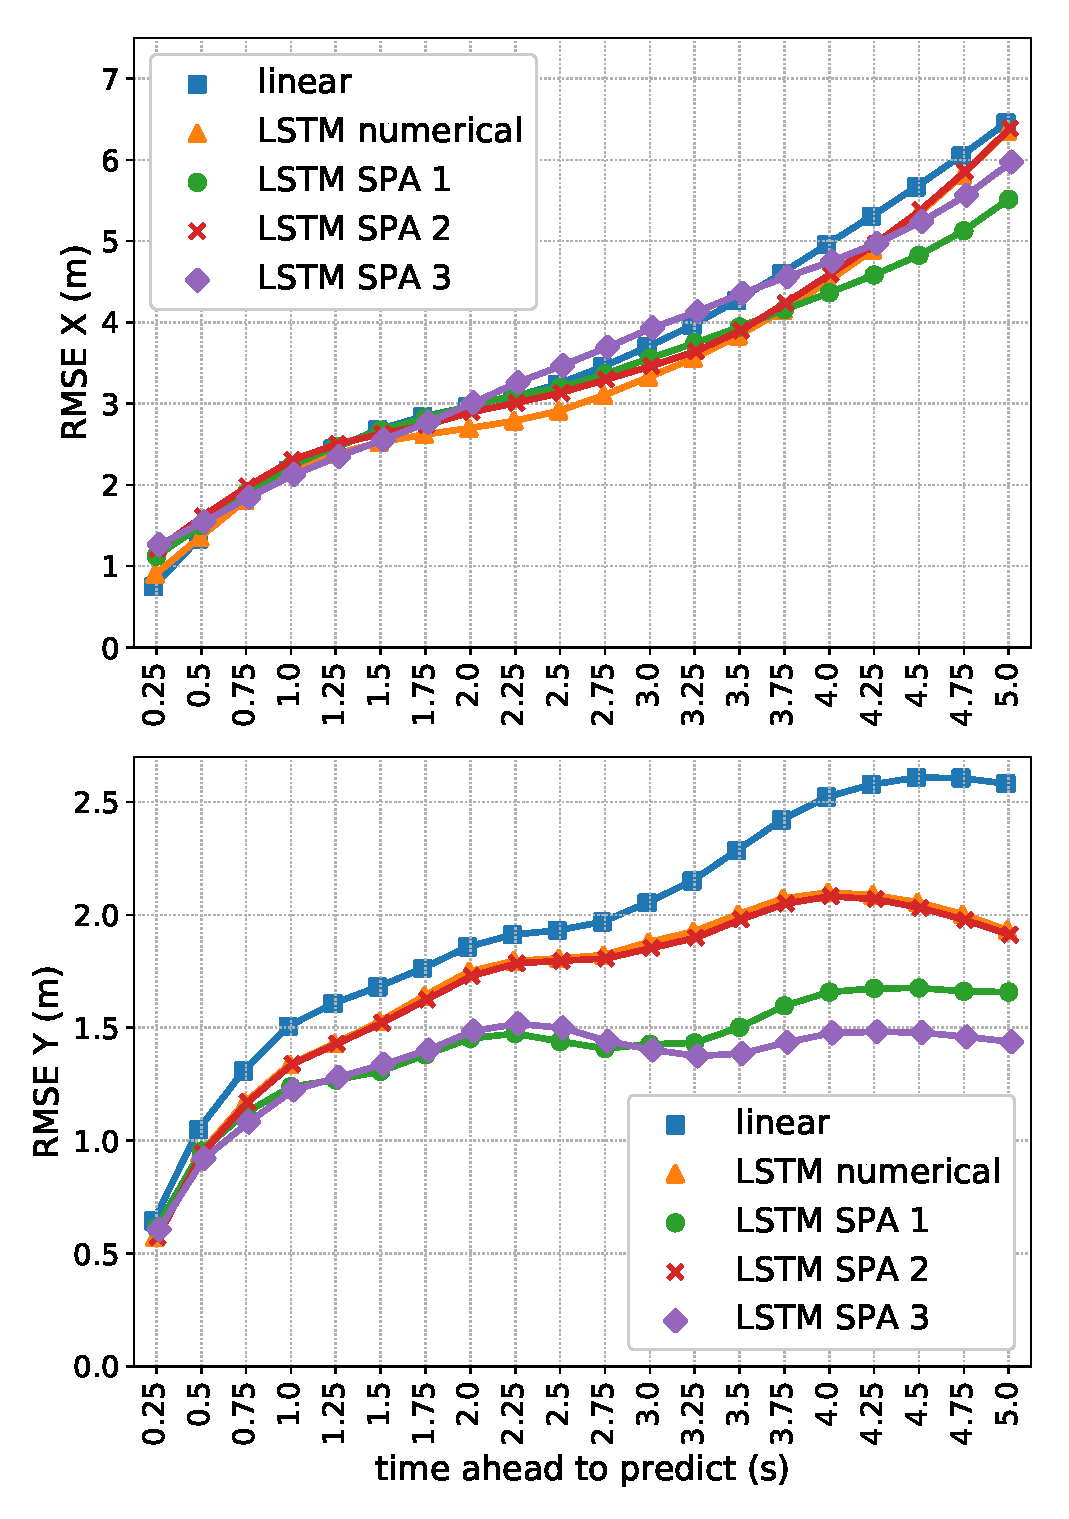
\includegraphics[width=0.25\linewidth]{imgs/rmse_large_subset_trained_on_lc_evaluated_on_lc.eps}
    }
    \caption{Visualization of the \ac{RMSE} performance of our \ac{LSTM} models for different data setups.
    Figures~\protect\subref{subfig:rmse_large_all},~\protect\subref{subfig:rmse_large_all_lc_only},~\protect\subref{subfig:rmse_large_subset} and~\protect\subref{subfig:rmse_large_subset_lc_only} show the \ac{RMSE} for models trained on the complete data set, while
Fig.~\protect\subref{subfig:rmse_large_all_trained_on_lc},~\protect\subref{subfig:rmse_large_all_lc_only_trained_on_lc},~\protect\subref{subfig:rmse_large_subset_trained_on_lc},~\protect\subref{subfig:rmse_large_subset_lc_only_trained_on_lc} show the same models evaluated on the same samples but trained only on the samples including a target vehicle lane change.}
    \label{fig:rmse_on_board_training_data_variation}
\end{figure}

In section~\ref{subsec:data_set_peculiarities}, we have already seen that our prediction models using neural networks have to deal with imbalanced data sets containing significantly more straight driving than lane changes performed by the target vehicle.
Hence, training any learning system on all the samples of both our data sets will expose the system to a significantly higher amount of data, in which most likely already a simple linear prediction model performs reasonably well. 
In this section, we therefore analyze the influence of the training data set on our \ac{LSTM} models and if there are significant differences in the performance of models trained on the complete data sets and on subsets consisting only of such samples that contain a lane change of the target vehicle.
We conduct this analysis on the \emph{On-board} data set only.
Figure~\ref{fig:rmse_on_board_all} showed the performance of our \ac{LSTM}-based models trained on the complete data set.
Here, we train models with the exact same neural network architectures and encoding schemes of the input just on different data sets, namely the subset of samples containing a lane change performed by the target vehicle.
We consider both types of target vehicle lane changes, namely those performed during the trajectory history as well as lane changes performed in the future trajectory to be predicted, as input for the models.
Figure~\ref{fig:rmse_on_board_training_data_variation} shows a comparison of different setups regarding training and evaluation data for our \ac{LSTM}-based trajectory prediction models.
We also keep the simple linear prediction model based on a constant velocity assumption for reference in the figures, since it is not a data-driven learning model and is therefore invariant under the changes of the training data.
Figures~\ref{subfig:rmse_large_all},~\ref{subfig:rmse_large_all_lc_only},~\ref{subfig:rmse_large_subset} and~\ref{subfig:rmse_large_subset_lc_only} show the \ac{RMSE} for models trained on the complete data set while Fig.~\ref{subfig:rmse_large_all_trained_on_lc},~\ref{subfig:rmse_large_all_lc_only_trained_on_lc},~\ref{subfig:rmse_large_subset_trained_on_lc} and~\ref{subfig:rmse_large_subset_lc_only_trained_on_lc} show the same models evaluated on the same samples but trained
only on data samples including a target vehicle lane change.
On the other hand, the upper row of Fig.~\ref{subfig:rmse_large_all} -~\ref{subfig:rmse_large_subset_trained_on_lc} illustrates the performance of the models trained on either the complete data set or on only the lane changes in all data samples, while the lower row of Fig.~\ref{subfig:rmse_large_all_lc_only} -~\ref{subfig:rmse_large_subset_lc_only_trained_on_lc} shows the performance of the models trained on either the complete data set or only on data samples containing a target vehicle lane change.

\begin{figure}[t!]
    \centering
    \subfloat[\label{subfig:rmse_large_all_spa_power_trained_on_lc_vs_trained_on_all}All samples]{%
        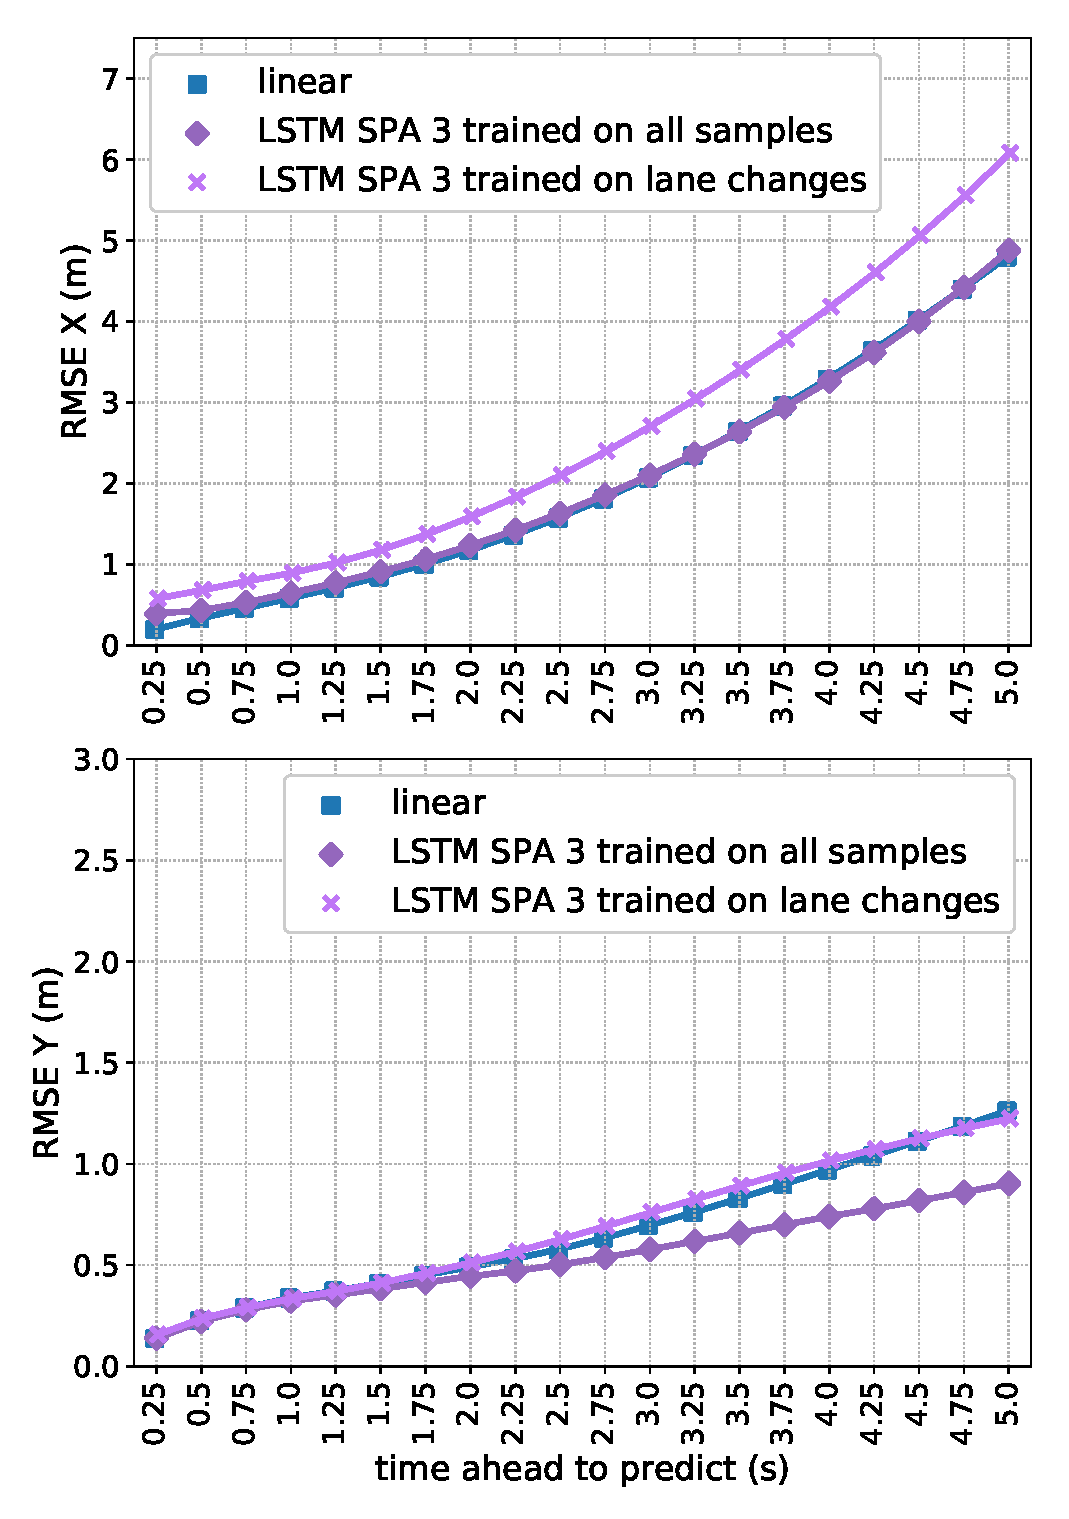
\includegraphics[width=0.25\linewidth]{imgs/rmse_large_all_spa_power_trained_on_lc_vs_trained_on_all.eps}
    }
    \subfloat[\label{subfig:rmse_large_all_lc_only_spa_power_trained_on_lc_vs_trained_on_all}Lane changes]{%
        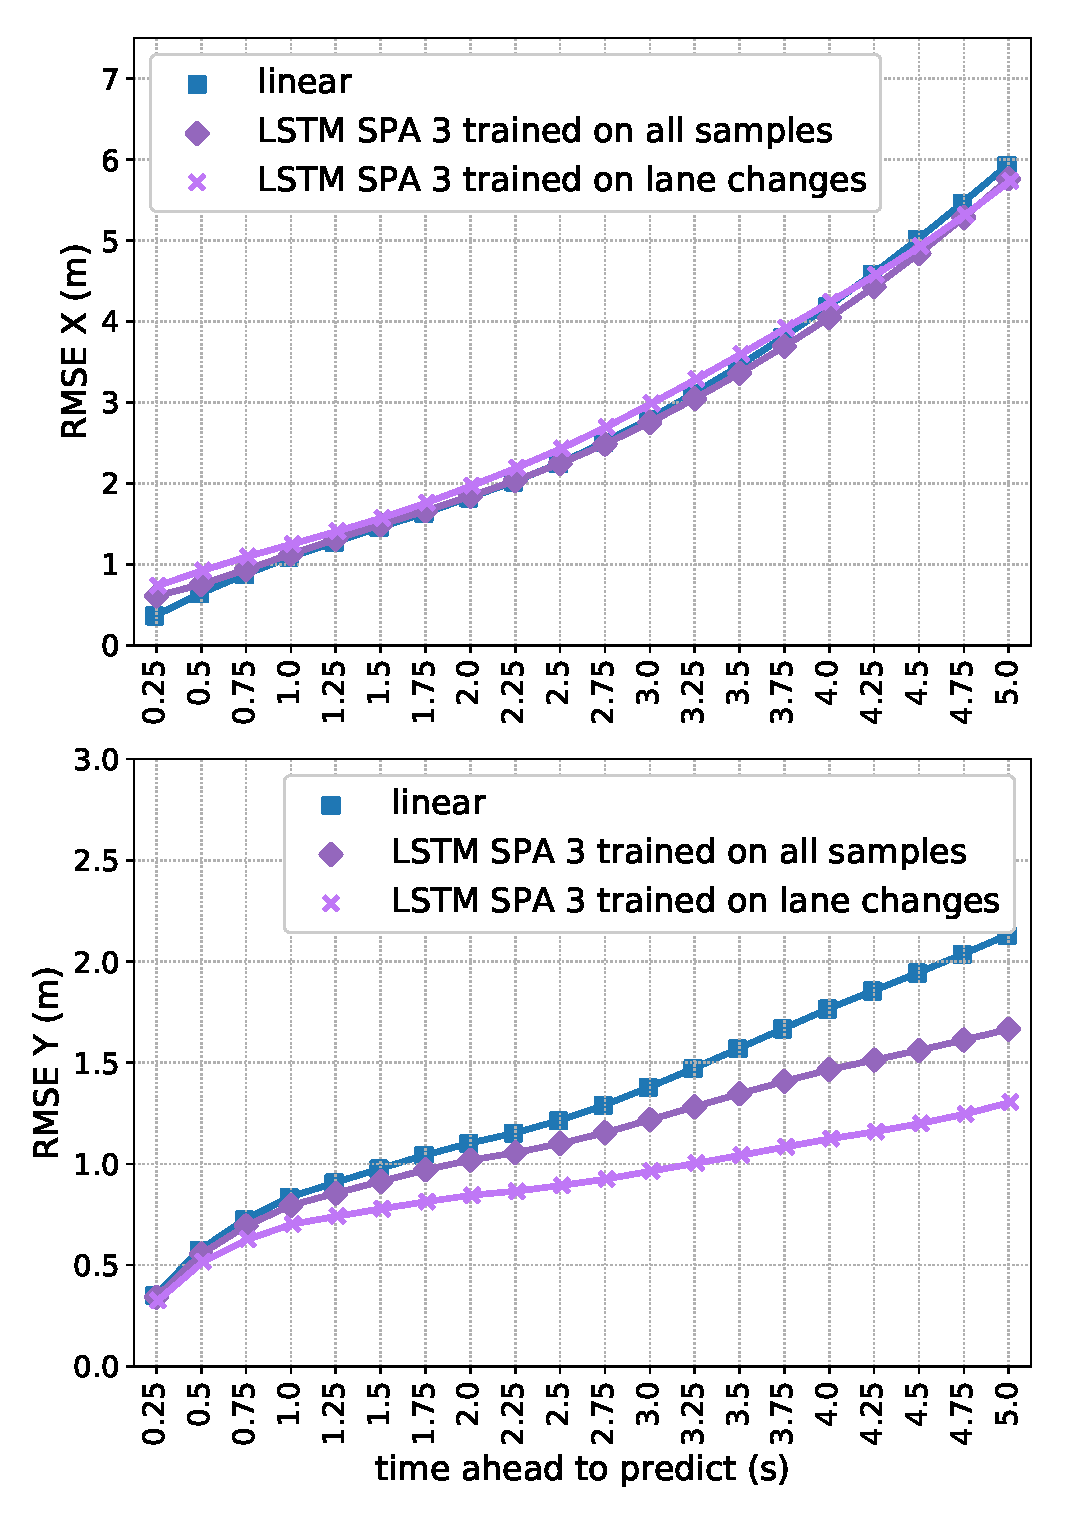
\includegraphics[width=0.25\linewidth]{imgs/rmse_large_all_lc_only_spa_power_trained_on_lc_vs_trained_on_all.eps}
    }
    \subfloat[\label{subfig:rmse_large_subset_spa_power_trained_on_lc_vs_trained_on_all}Crowded]{%
        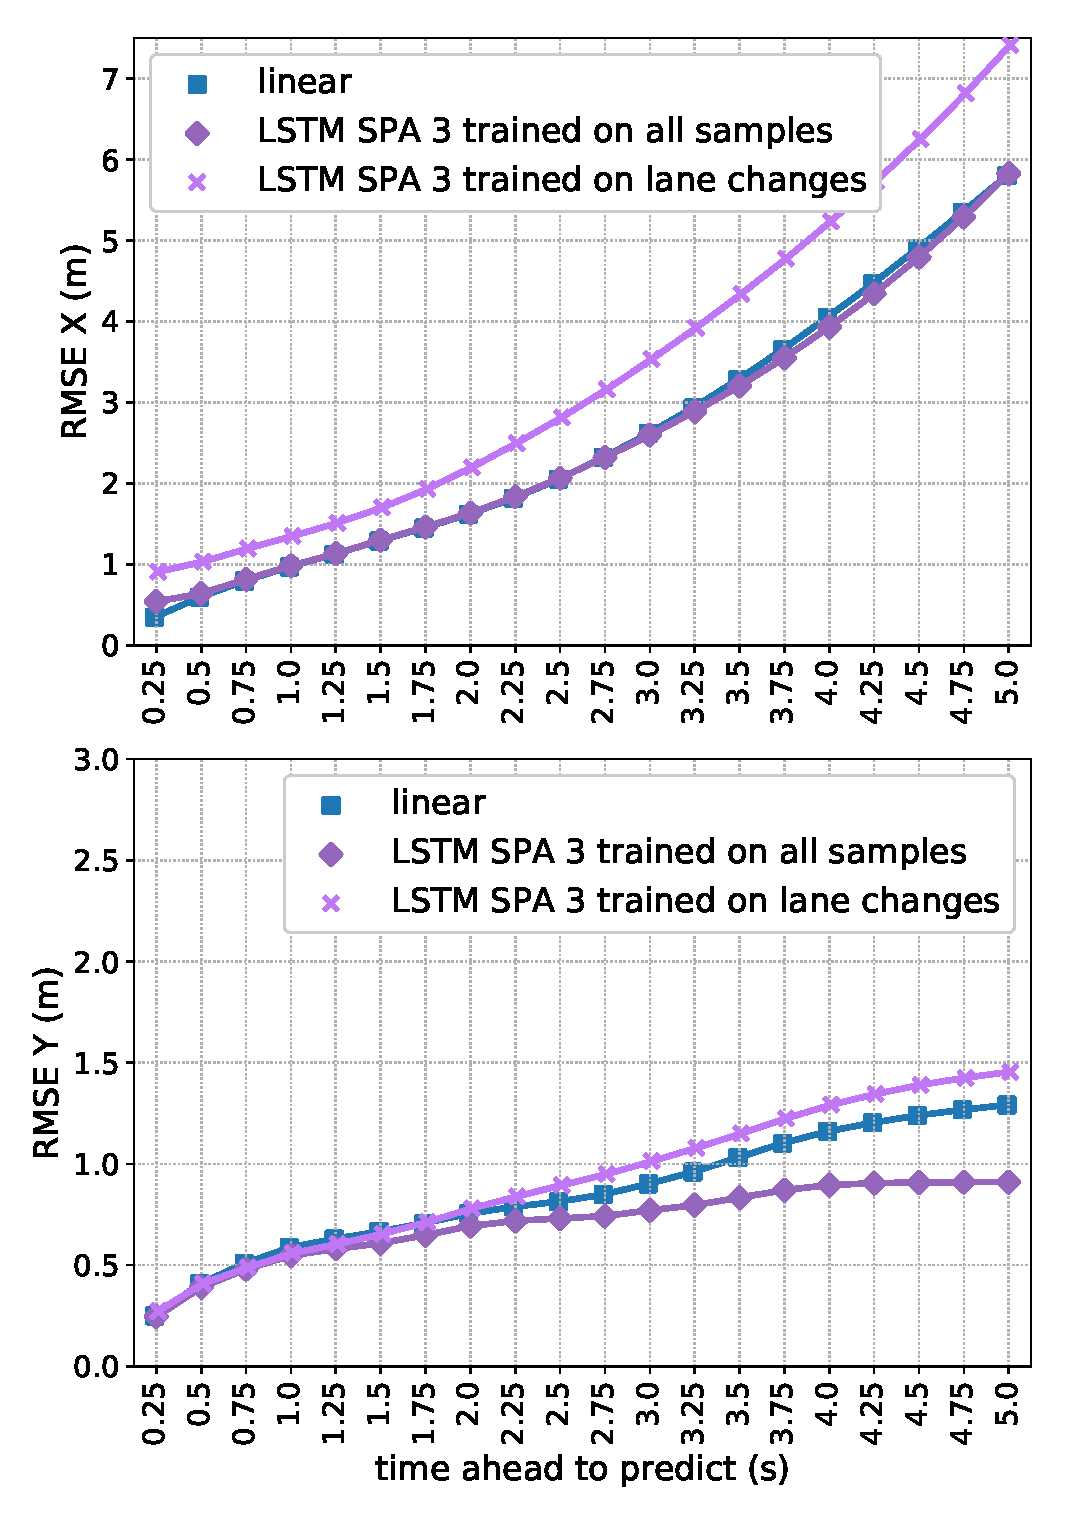
\includegraphics[width=0.25\linewidth]{imgs/rmse_large_subset_spa_power_trained_on_lc_vs_trained_on_all.eps}
    }
    \subfloat[\label{subfig:rmse_large_subset_lc_only_spa_power_trained_on_lc_vs_trained_on_all}Crowded lane changes]{%
        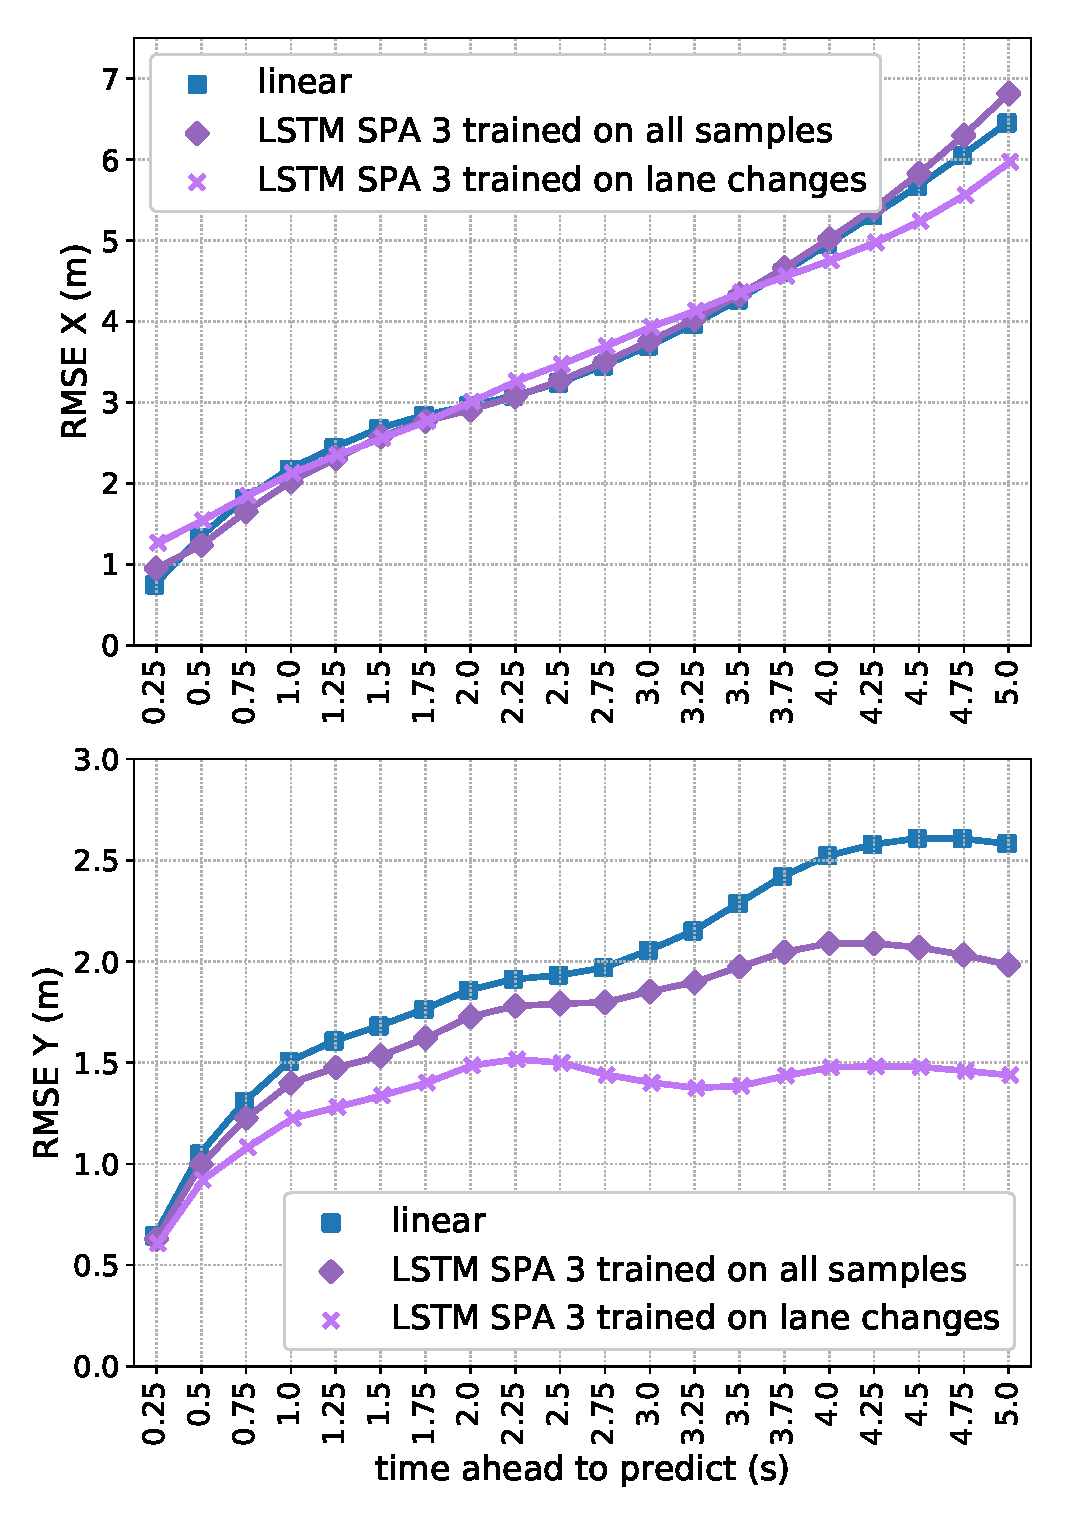
\includegraphics[width=0.25\linewidth]{imgs/rmse_large_subset_lc_only_spa_power_trained_on_lc_vs_trained_on_all.eps}
    }\\
    \subfloat[\label{subfig:rmse_large_all_numerical_trained_on_lc_vs_trained_on_all}All samples]{%
        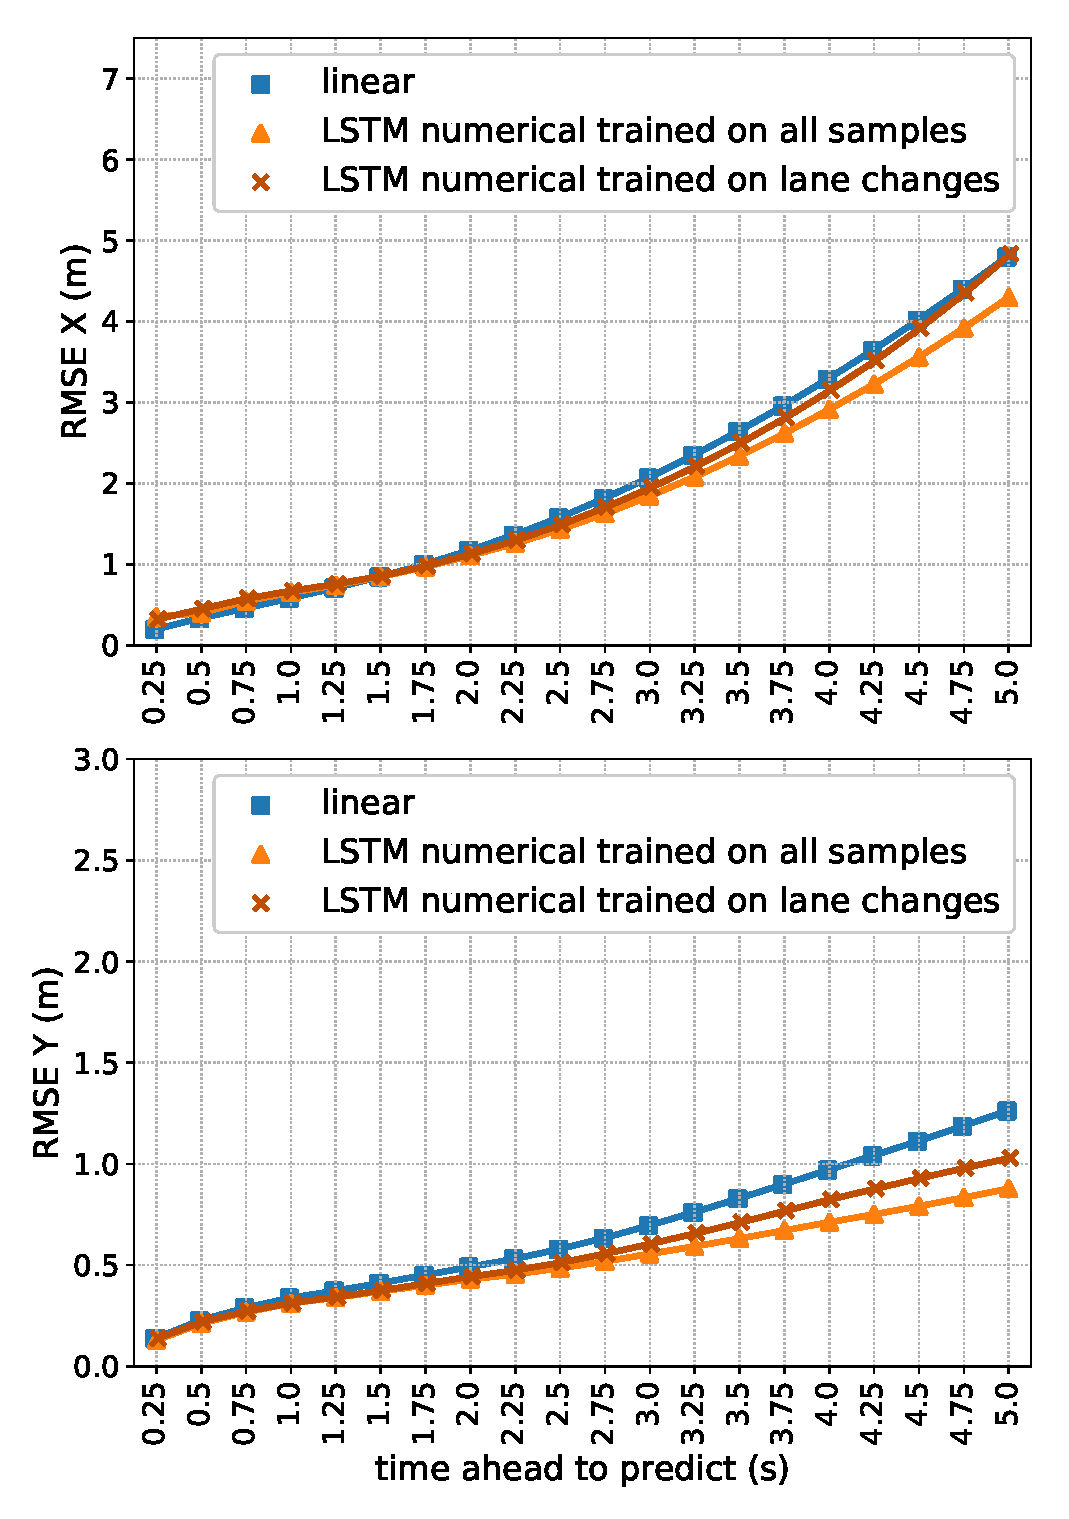
\includegraphics[width=0.25\linewidth]{imgs/rmse_large_all_numerical_trained_on_lc_vs_trained_on_all.eps}
    }
    \subfloat[\label{subfig:rmse_large_all_lc_only_numerical_trained_on_lc_vs_trained_on_all}Lane changes]{%
        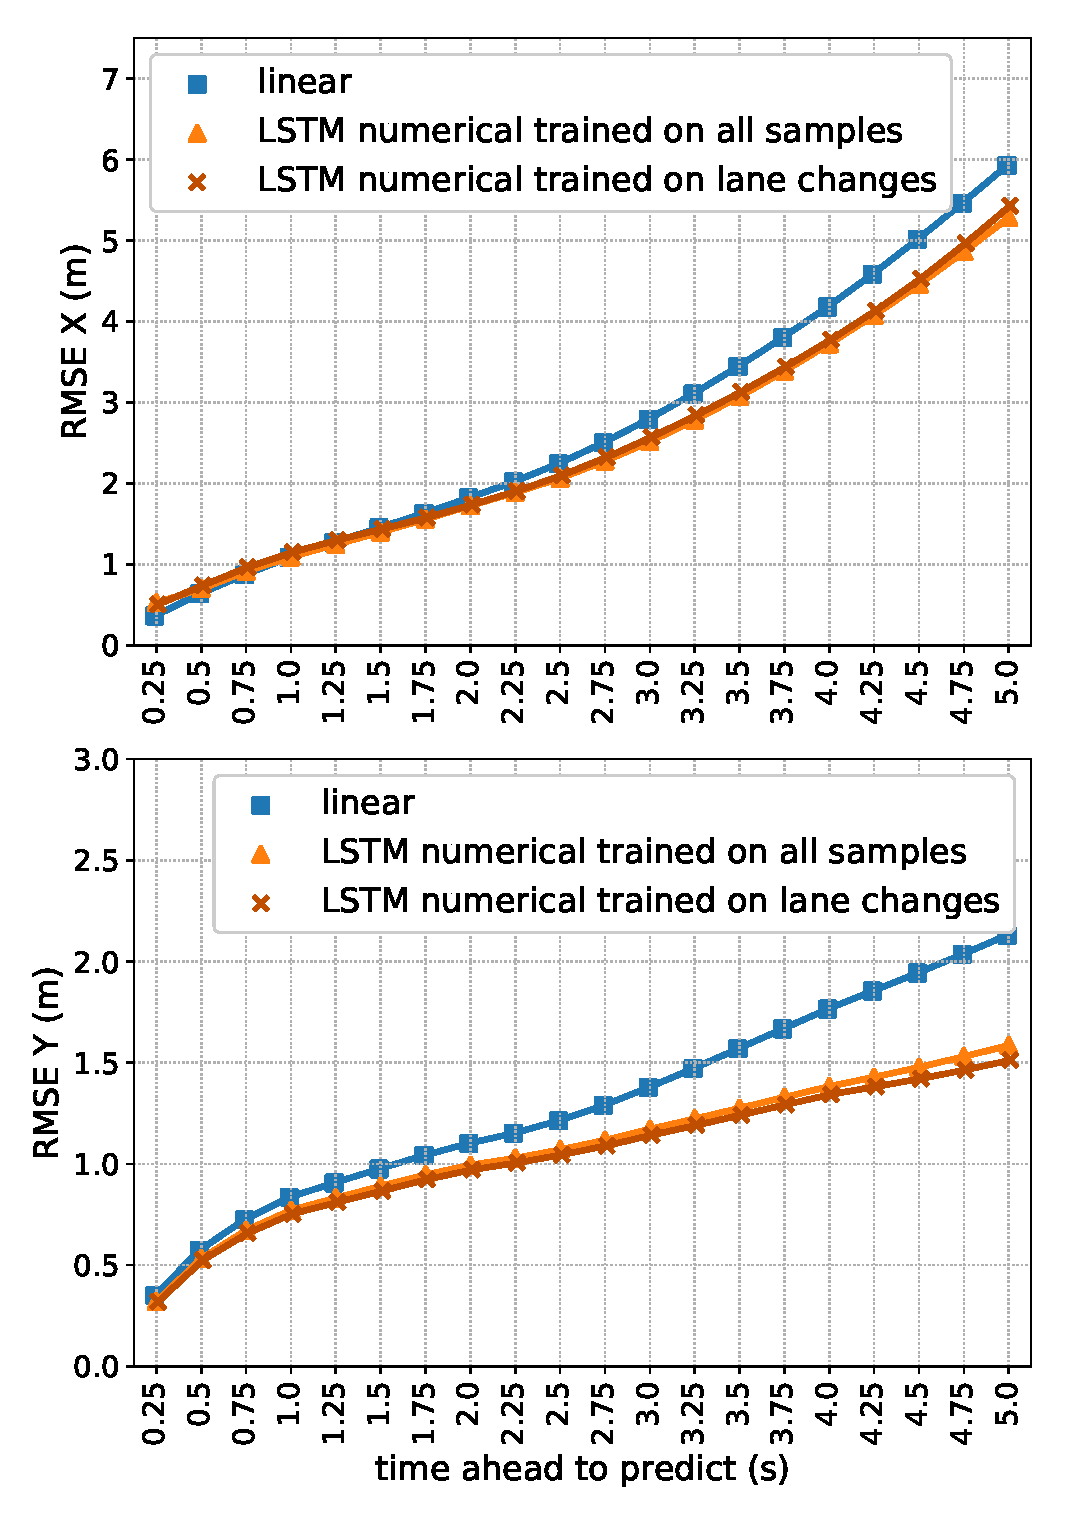
\includegraphics[width=0.25\linewidth]{imgs/rmse_large_all_lc_only_numerical_trained_on_lc_vs_trained_on_all.eps}
    }
    \subfloat[\label{subfig:rmse_large_subset_numerical_trained_on_lc_vs_trained_on_all}Crowded]{%
        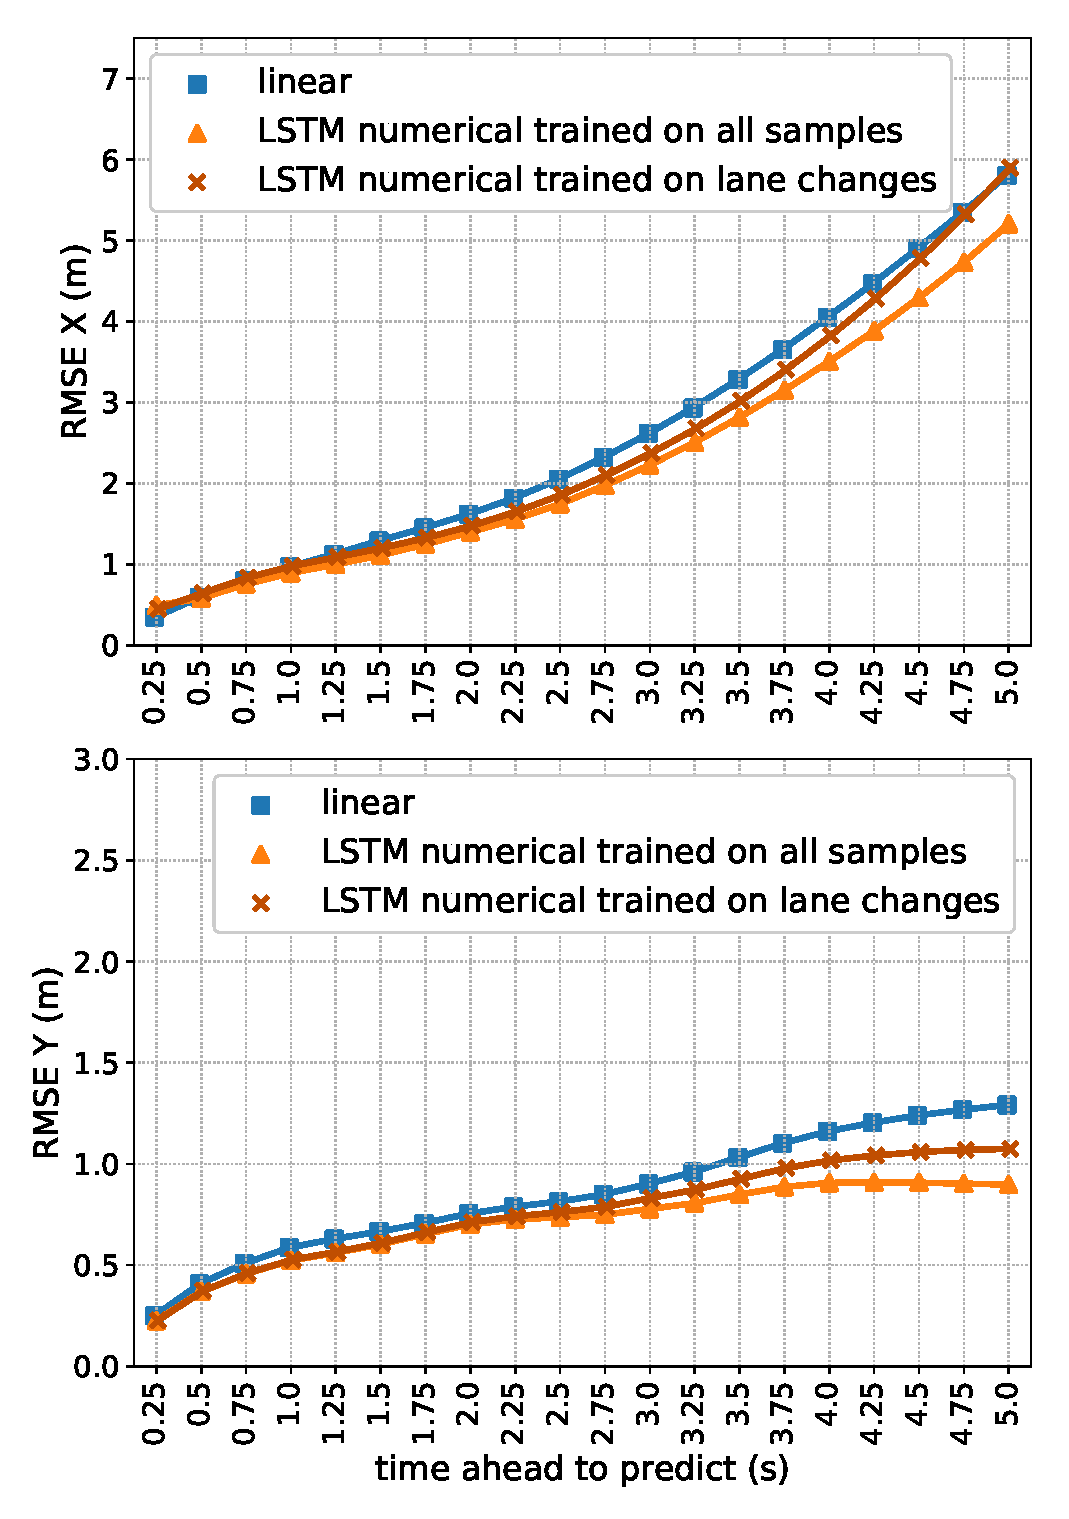
\includegraphics[width=0.25\linewidth]{imgs/rmse_large_subset_numerical_trained_on_lc_vs_trained_on_all.eps}
    }
    \subfloat[\label{subfig:rmse_large_subset_lc_only_numerical_trained_on_lc_vs_trained_on_all}Crowded lane changes]{%
        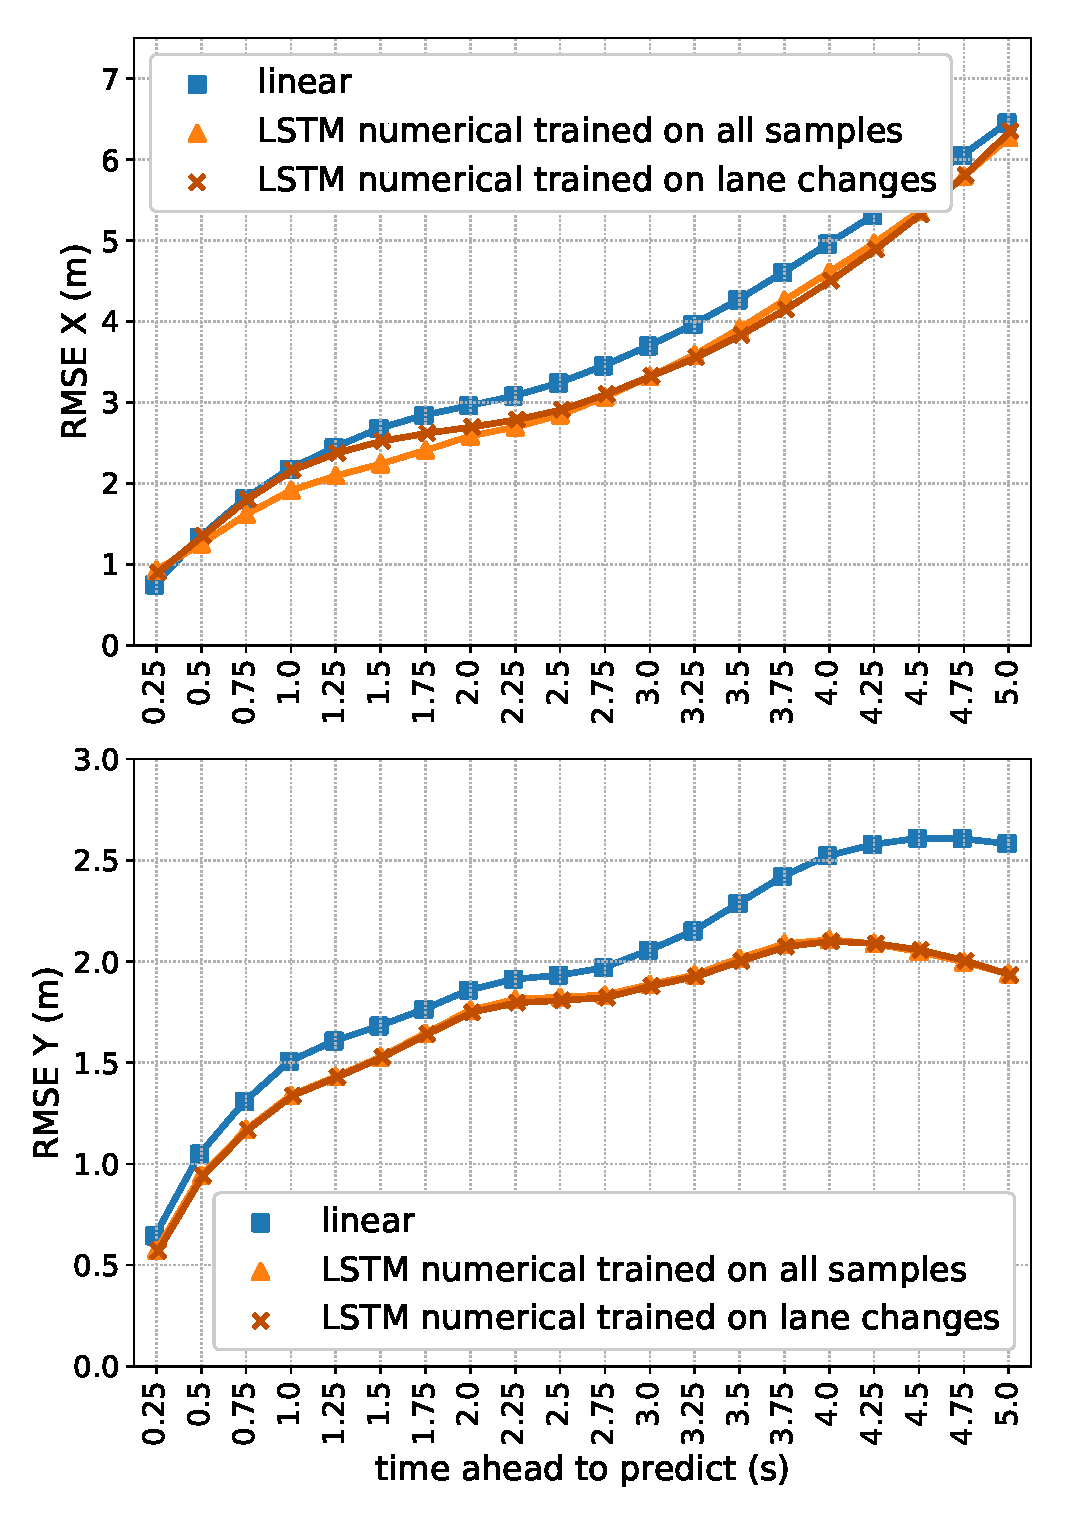
\includegraphics[width=0.25\linewidth]{imgs/rmse_large_subset_lc_only_numerical_trained_on_lc_vs_trained_on_all.eps}
    }
    \caption{Visualization of the changing \ac{RMSE} performance of particular prediction models depending on the data they have been trained on.
        The first four figures~\protect\subref{subfig:rmse_large_all_spa_power_trained_on_lc_vs_trained_on_all} -~\protect\subref{subfig:rmse_large_subset_lc_only_spa_power_trained_on_lc_vs_trained_on_all} illustrate the difference between the \ac{LSTM} \acs{SPA} \num{3} models when changing their training data, while the last four figures~\protect\subref{subfig:rmse_large_all_numerical_trained_on_lc_vs_trained_on_all} -
        ~\protect\subref{subfig:rmse_large_subset_lc_only_numerical_trained_on_lc_vs_trained_on_all} shows the same comparison for the \ac{LSTM} numerical models.
    }
    \label{fig:rmse_on_board_training_all_vs_training_on_lc_only}
\end{figure}

We observe that the models that have been trained only on samples containing a lane change performed by the target vehicle tend to achieve worse results than the models trained on the complete data set, when being evaluated on the entirety of all data samples (Fig.~\ref{subfig:rmse_large_all},~\ref{subfig:rmse_large_subset},~\ref{subfig:rmse_large_all_lc_only} and~\ref{subfig:rmse_large_subset_lc_only}).
Interestingly, the performance of the models based on the convolutive power encoding scheme (\acs{LSTM} \acs{SPA} \num{1} and \num{3}) deteriorates more significantly compared to the other data-driven models, especially in lateral ($y$) direction.
However, if we evaluate the same models only on the samples containing a target vehicle lane change, their performance changes significantly (Fig.~\ref{subfig:rmse_large_all_lc_only} -~\ref{subfig:rmse_large_subset_lc_only_trained_on_lc}).
We recapitulate the findings of section~\ref{subsec:data_set_peculiarities} that lane changes influence the lateral ($y$) position values more severely than the longitudinal ($x$) position compared to straight driving samples.
Therefore, the performance difference between the models trained on lane changes only and models trained on the complete data set, as we would expect, is also not that significant in longitudinal direction.
Considering the lateral ($y$) direction however, we observe a significant change between both model and evaluation variants.
If the models are trained only on lane change samples, the \ac{LSTM} \acs{SPA} \num{1} and \num{3} models outperform all other models in lateral direction when evaluated only on the data samples containing a lane change while their performance in longitudinal direction does not change significantly compared to the models trained on the complete data set.

So far, we have only compared either all models trained on the complete data set or all models trained only on the lane change samples.
However, we are also interested in how the performance for particular models changes when modifying the training data set.
Figure~\ref{fig:rmse_on_board_training_all_vs_training_on_lc_only} shows a comparison of the \ac{LSTM}-based models when modifying the training data for the \ac{LSTM} \acs{SPA} \num{3} model (Fig.~\ref{subfig:rmse_large_all_spa_power_trained_on_lc_vs_trained_on_all} -~\ref{subfig:rmse_large_subset_lc_only_spa_power_trained_on_lc_vs_trained_on_all}) as well as the \acs{LSTM} numerical model (Fig.
~\ref{subfig:rmse_large_all_numerical_trained_on_lc_vs_trained_on_all} -~\ref{subfig:rmse_large_subset_lc_only_numerical_trained_on_lc_vs_trained_on_all}).
In this direct comparison, we observe that there is no significant difference in the performance of the numerical \ac{LSTM} models trained on different samples for both evaluation sets containing either the complete data set or only the target vehicle lane changes.
For the \ac{LSTM} \acs{SPA} \num{3} model however, we observe significant improvements for the model trained on the lane change samples when evaluated on the lane changes performed by the target vehicle the model trained on all data samples.
This result indicates that either the numerical model trained on all samples generalizes sufficiently well to all possible situations compared to the convolutive power based model.
However, we have already seen, that both trajectory data sets show a significant imbalance towards straight driving compared to lane change maneuvers (cf.\ section~\ref{subsec:data_set_peculiarities}), which is the same for all models.
On the other hand, the results shown here could also hint, that the convolutive power model encapsulating the prior motion not only of the target vehicle but also other vehicles in its surroundings is better suited to predict lane change maneuvers given a more balanced data set.
These results suggest, that there is not only room for improvement for the models investigated here, but also other data-driven models used for trajectory prediction in the literature, by researching and evaluating the influence of the distribution of driving situations within the training data.

\subsection{Evaluation of \acs{NEF}-based feed-forward prediction models}%
\label{subsec:evaluation_of_nef_based_feed_forward_prediction_models}

In this section, we evaluate the simpler, feed-forward neural networks for trajectory prediction to compare our \ac{LSTM}-based models to.

\subsubsection{Hyperparameter analysis}%
\label{ssubsec:hyperparameter_analysis_nef}

\begin{figure}[t!]
  \centering
  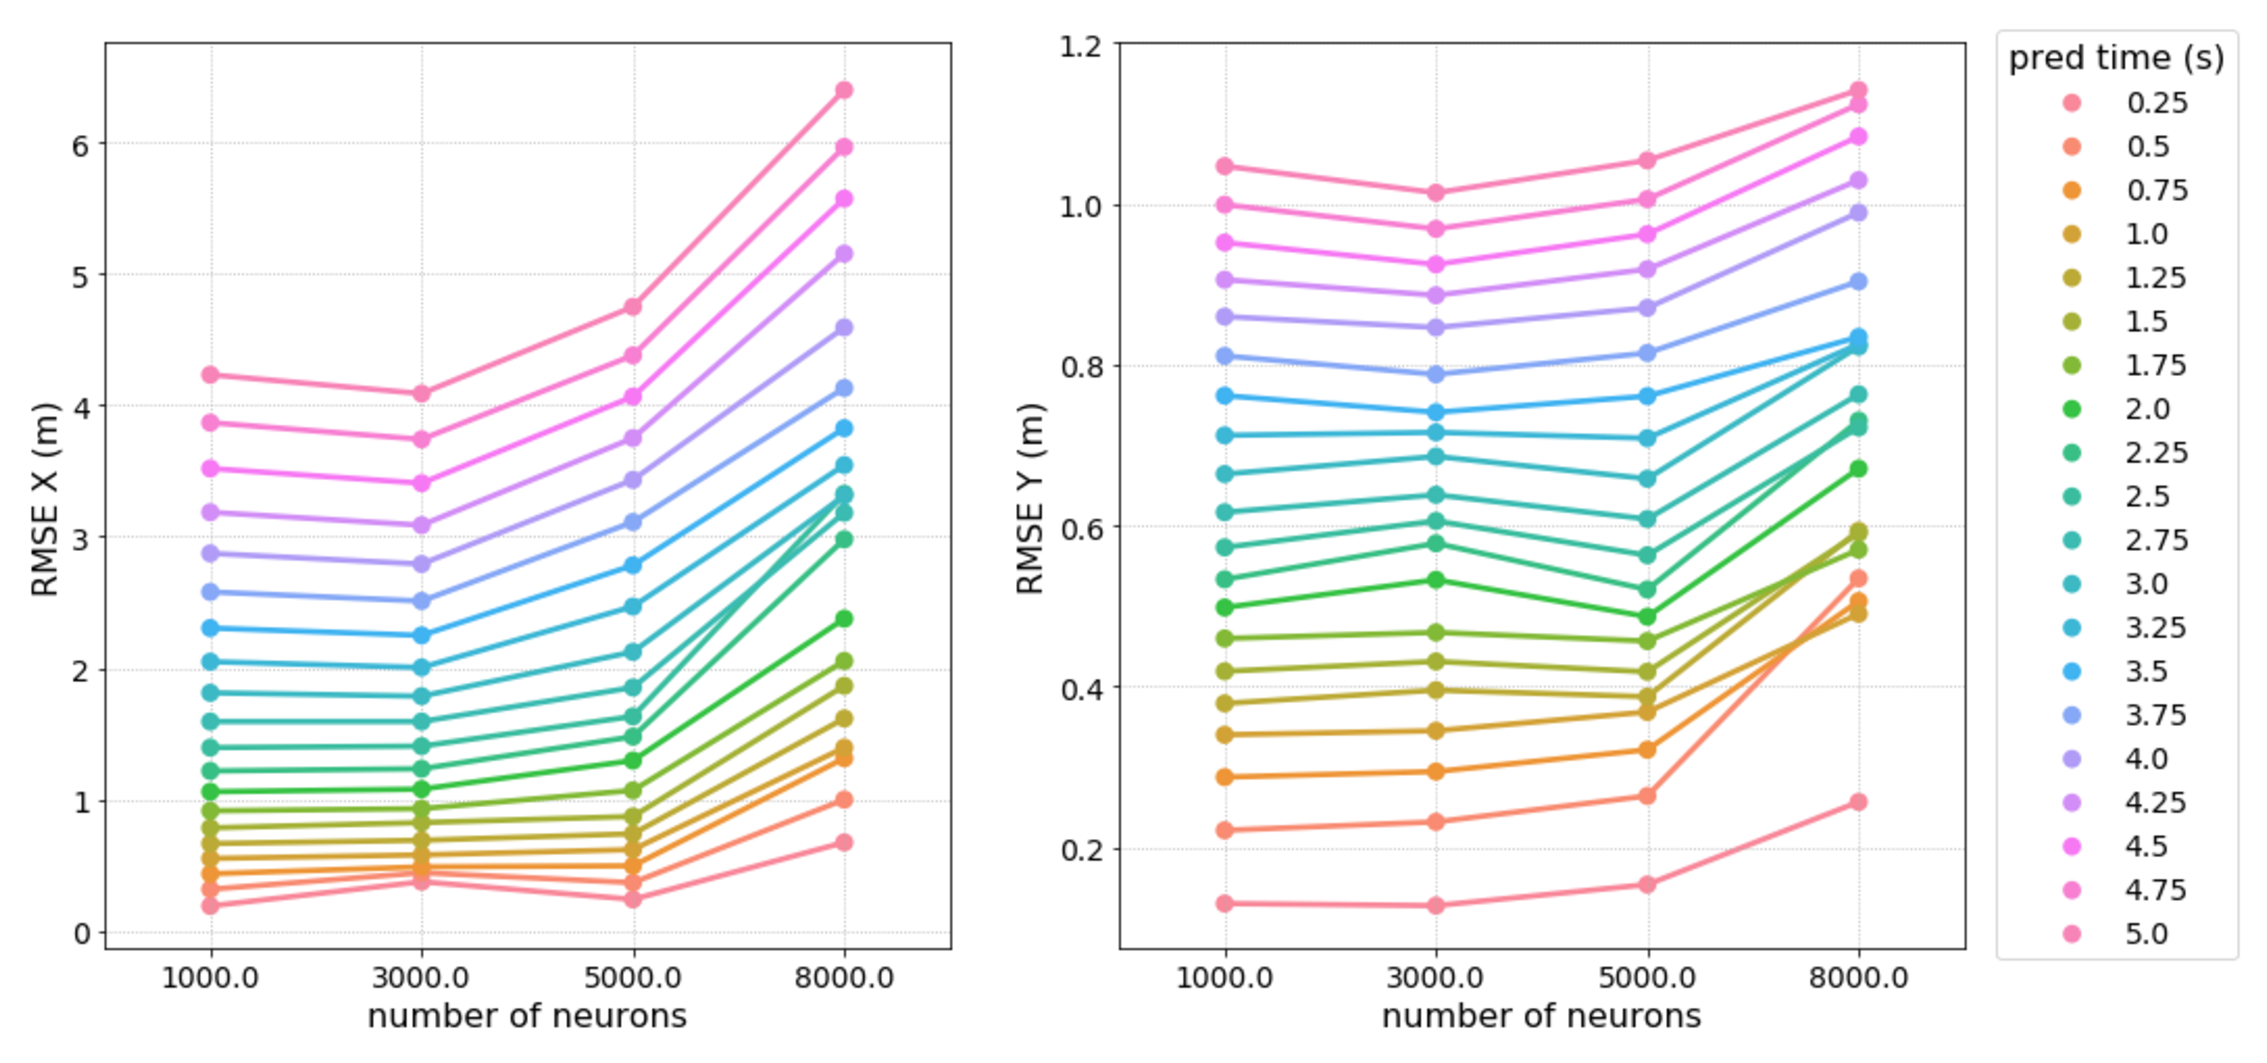
\includegraphics[width=0.95\textwidth]{imgs/nef_num_neurons_analysis.eps}
  \caption{Analysis of the \ac{RMSE} for a varying number of neurons in the learning population of our \ac{NEF} model trained on numerical input from the \emph{On-board} data set.}
  \label{fig:nef_num_neurons_analysis}
\end{figure}

For our \ac{NEF} networks, the main parameter influencing the models' performance is the number of neurons in the learning population, i.e., the hidden layer in terms of traditional neural networks, as well as the neuron model.
For simplicity, we use \acs{Nengo}'s rate-variant of the \ac{LIF} neuron model.
Here, we inspect the number of neurons in the learning population in more detail.
From the \ac{NEF}-theory \parencite{Eliasmith2003} we know that increasing the number of neurons in a population yields a more accurate representation of the data encoded in the population's activity.
Thus, we expect more accurate predictions when increasing the number of neurons.
Figure~\ref{fig:nef_num_neurons_analysis} shows the \ac{RMSE} of different model instantiations with varying number of neurons, namely \num{1000}, \num{3000}, \num{5000} and \num{8000} neurons.
We observe that a number of \num{3000} spiking neurons is sufficient and further increasing the number of neurons does not improve the model's prediction accuracy.
Note that the order of magnitude of the \ac{RMSE} in Fig.~\ref{fig:nef_num_neurons_analysis} is significantly higher than for the figures visualizing the \ac{LSTM} models \ac{RMSE} inspected in the previous section. 
This is due to the fact that the \ac{NEF} models investigated here receive less amount of information, namely only position data and instantaneous velocity of the target vehicle, compared to the \ac{LSTM} models.
Here, we are only interested to find the best possible parameter setup, whereas we will evaluate both models with comparable setups in later sections.

\subsubsection{Model training}%
\label{ssubsec:model_training_nef}

We train two different variants of our simpler \ac{NEF}-models using numerical input (\acs{NEF} numerical) as well as the \ac{SPA}-power-with-ego (\acs{NEF} \acs{SPA} \num{1}) and \ac{SPA}-power encoding (\acs{NEF} \acs{SPA} \num{2}) for the \emph{On-board} and the \emph{\ac{NGSIM}} data set respectively.
The neural weights are calculated using \acs{Nengo}'s default least-squares-optimization method with the exception, that we calculate the weights over smaller subsets of the input data for computational reasons.
Here, we adapt the input data such that for the numerical \ac{NEF}-model, we use the vector $(x_{t_{0}}, \ldots, x_{t_{N}}, y_{t_{0}}, \ldots, y_{t_{N}}, v)$ as input with $v$ denoting the instantaneous velocity of the target vehicle.
For the \ac{SPA}-power encoding schemes, instead of flattening the whole sequence of vectors into one giant single vector, we created a single semantic vector by summing the first, middle and last element of the original vector sequences

\begin{equation}
  \hat{\mathbf{S}} =  \mathbf{S}_{t_0} \oplus \mathbf{S}_{t_{\nicefrac{N}{2}}} \oplus \mathbf{S}_{t_N} = (\hat{s}_0, \ldots, \hat{s}_{D-1}).
\end{equation}
We only sum up these vectors instead of the whole sequence $(\mathbf{S}_{t})_{t_0}^{t_N}$ to avoid the accumulation of noise in the vector representation.
Note that thereby the \ac{NEF} model using the \ac{SPA}-power representation does not use the full trajectory history but only selected time steps, namely those visualized in Fig.~\ref{fig:spa_power}.
We also include the instantaneous velocity $v$ of the target vehicle as an additional vector element, which yields $(\hat{s}_0, \ldots, \hat{s}_{D-1}, v)$ as input of our model.
To make these simpler models as comparable as possible to the \ac{LSTM} models in terms of information available to the network, we add the instantaneously velocity of the target vehicle as an additional element to the input, since there is no intermediate embedding vector here where it could be included.

\subsubsection{Evaluation}%
\label{ssubsec:evaluation_nef}

\begin{figure}[t!]
	\centering
    \subfloat[\label{subfig:nef_rmse_512_onboard}]{%
        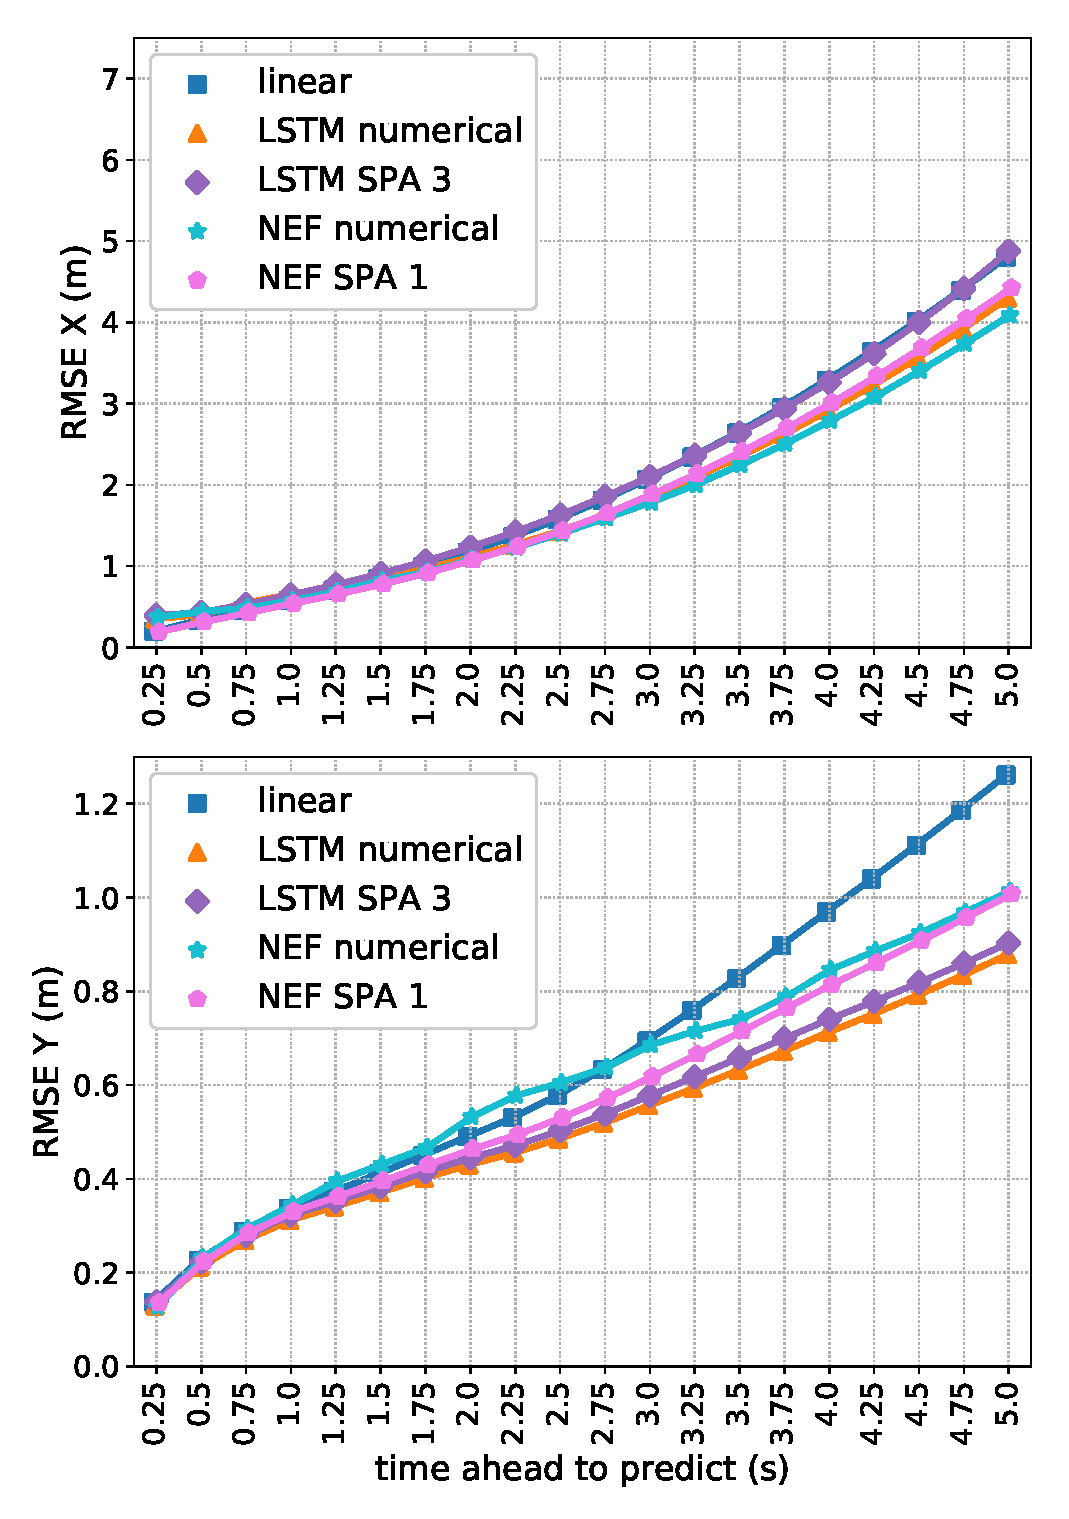
\includegraphics[width=0.5\columnwidth]{imgs/rmse_on_board_nef_nets.eps}
    }
    \subfloat[\label{subfig:nef_rmse_1024_ngsim}]{%
        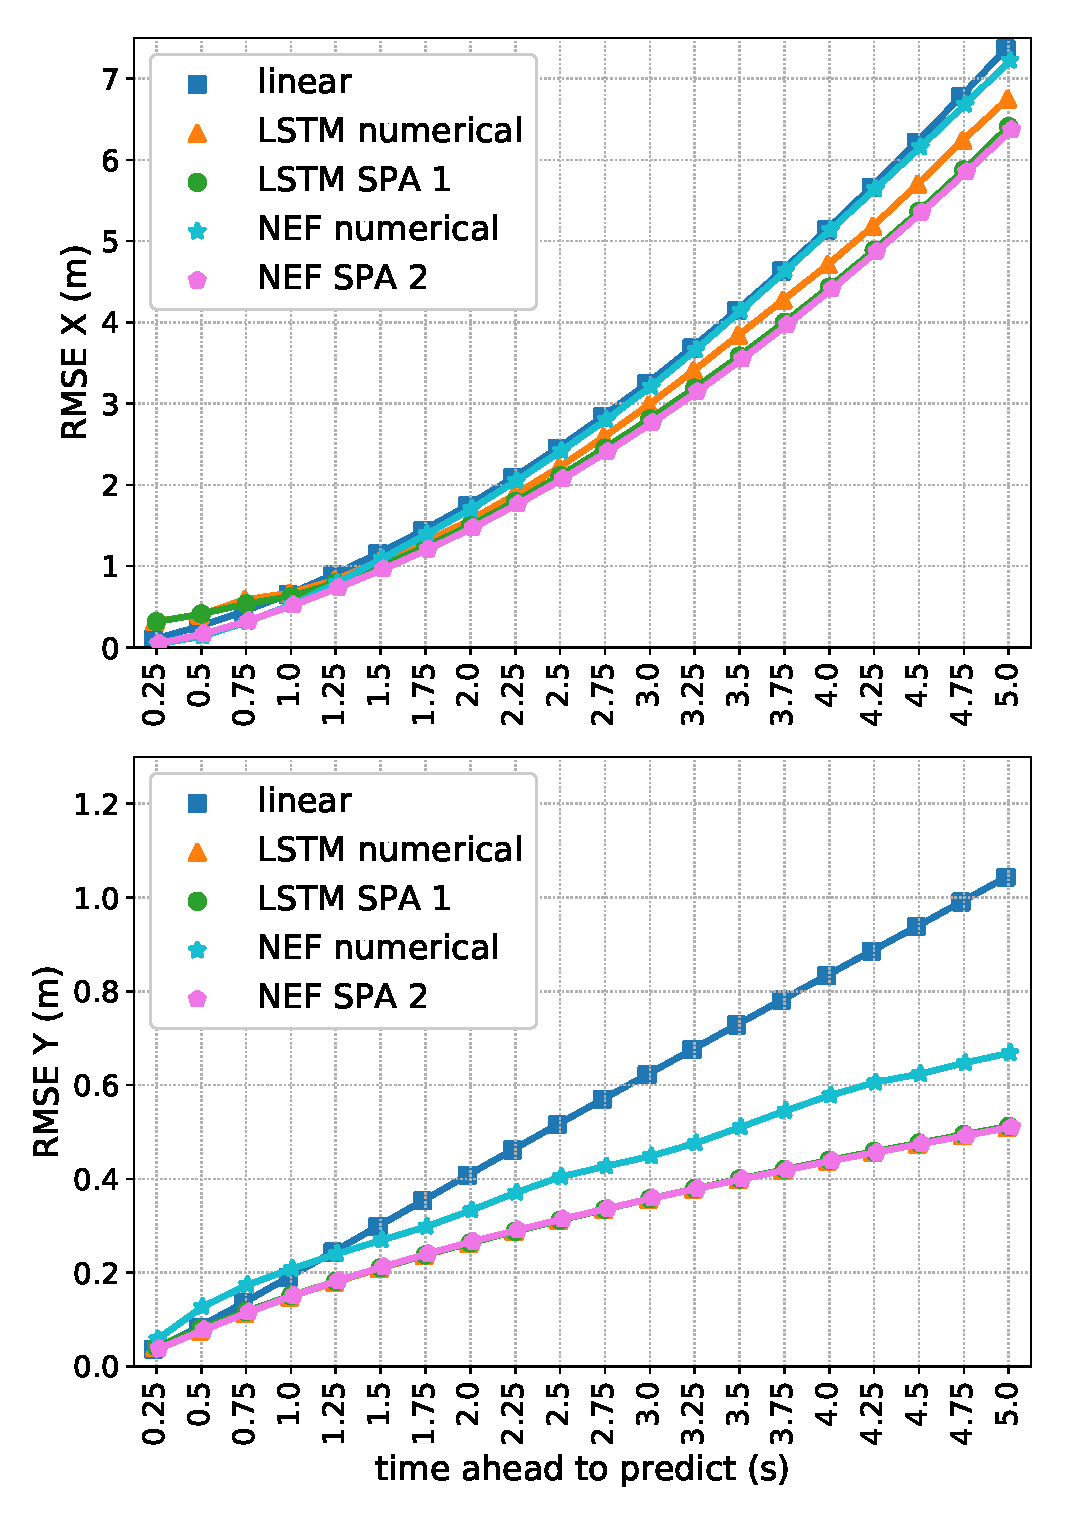
\includegraphics[width=0.5\columnwidth]{imgs/rmse_ngsim_nef_nets.eps}
    }
    \caption{Visualization of the \ac{RMSE} of all \ac{NEF}-network models~\protect\subref{subfig:nef_rmse_512_onboard} on the \emph{On-board} validation set $V_1 \subset D_1$ using \num{512}-dimensional vectors for the \ac{SPA}-power vectors and~\protect\subref{subfig:nef_rmse_1024_ngsim} on the \emph{\ac{NGSIM}} data set $D_2$ using \num{1024}-dimensional vectors for the \ac{SPA}-power vectors.}\label{fig:rmse_nef_nets}

\end{figure}

Figure~\ref{fig:rmse_nef_nets} visualizes the \ac{RMSE} of our \ac{NEF}-network models on both data sets.
The \ac{NEF}-network using the \ac{SPA}-power encoding schemes processes \num{512}-dimensional for the \emph{On-board} (\ac{NEF} \ac{SPA} \num{1}) and \num{1024}-dimensional vectors for the \emph{\ac{NGSIM}} data set (\ac{NEF} \ac{SPA} \num{2}).
For reference, we included the performance of the most relevant \ac{LSTM} models, namely \ac{LSTM} \ac{SPA} \num{1} and \num{3} for the \emph{\ac{NGSIM}} and \emph{On-board} data set respectively as well as \ac{LSTM} numerical, in Fig.~\ref{fig:rmse_nef_nets} as well.
We observe that, despite a simpler network architecture and learning algorithm, the \ac{NEF}-networks achieve a performance comparable to the more sophisticated \ac{LSTM} models on both data sets.
For the \emph{\ac{NGSIM}} data set, the \ac{NEF} \ac{SPA} \num{1} model performs on par with its \ac{LSTM} model counterpart \ac{LSTM} \ac{SPA} \num{3}.
In this case, the \ac{NEF}-model is not only simpler, but also has access to less information as its input data is a sum of a subset of the input sequence used for the corresponding \ac{LSTM}-model.

\subsection{Evaluation of the unsupervised anomaly detection}%
\label{subsec:evaluation_of_the_unsupervised_anomaly_detection}

\begin{figure}[t]
    \centering
    \subfloat[\label{subfig:anomalies_on_board_boxplots_distances}]{%
        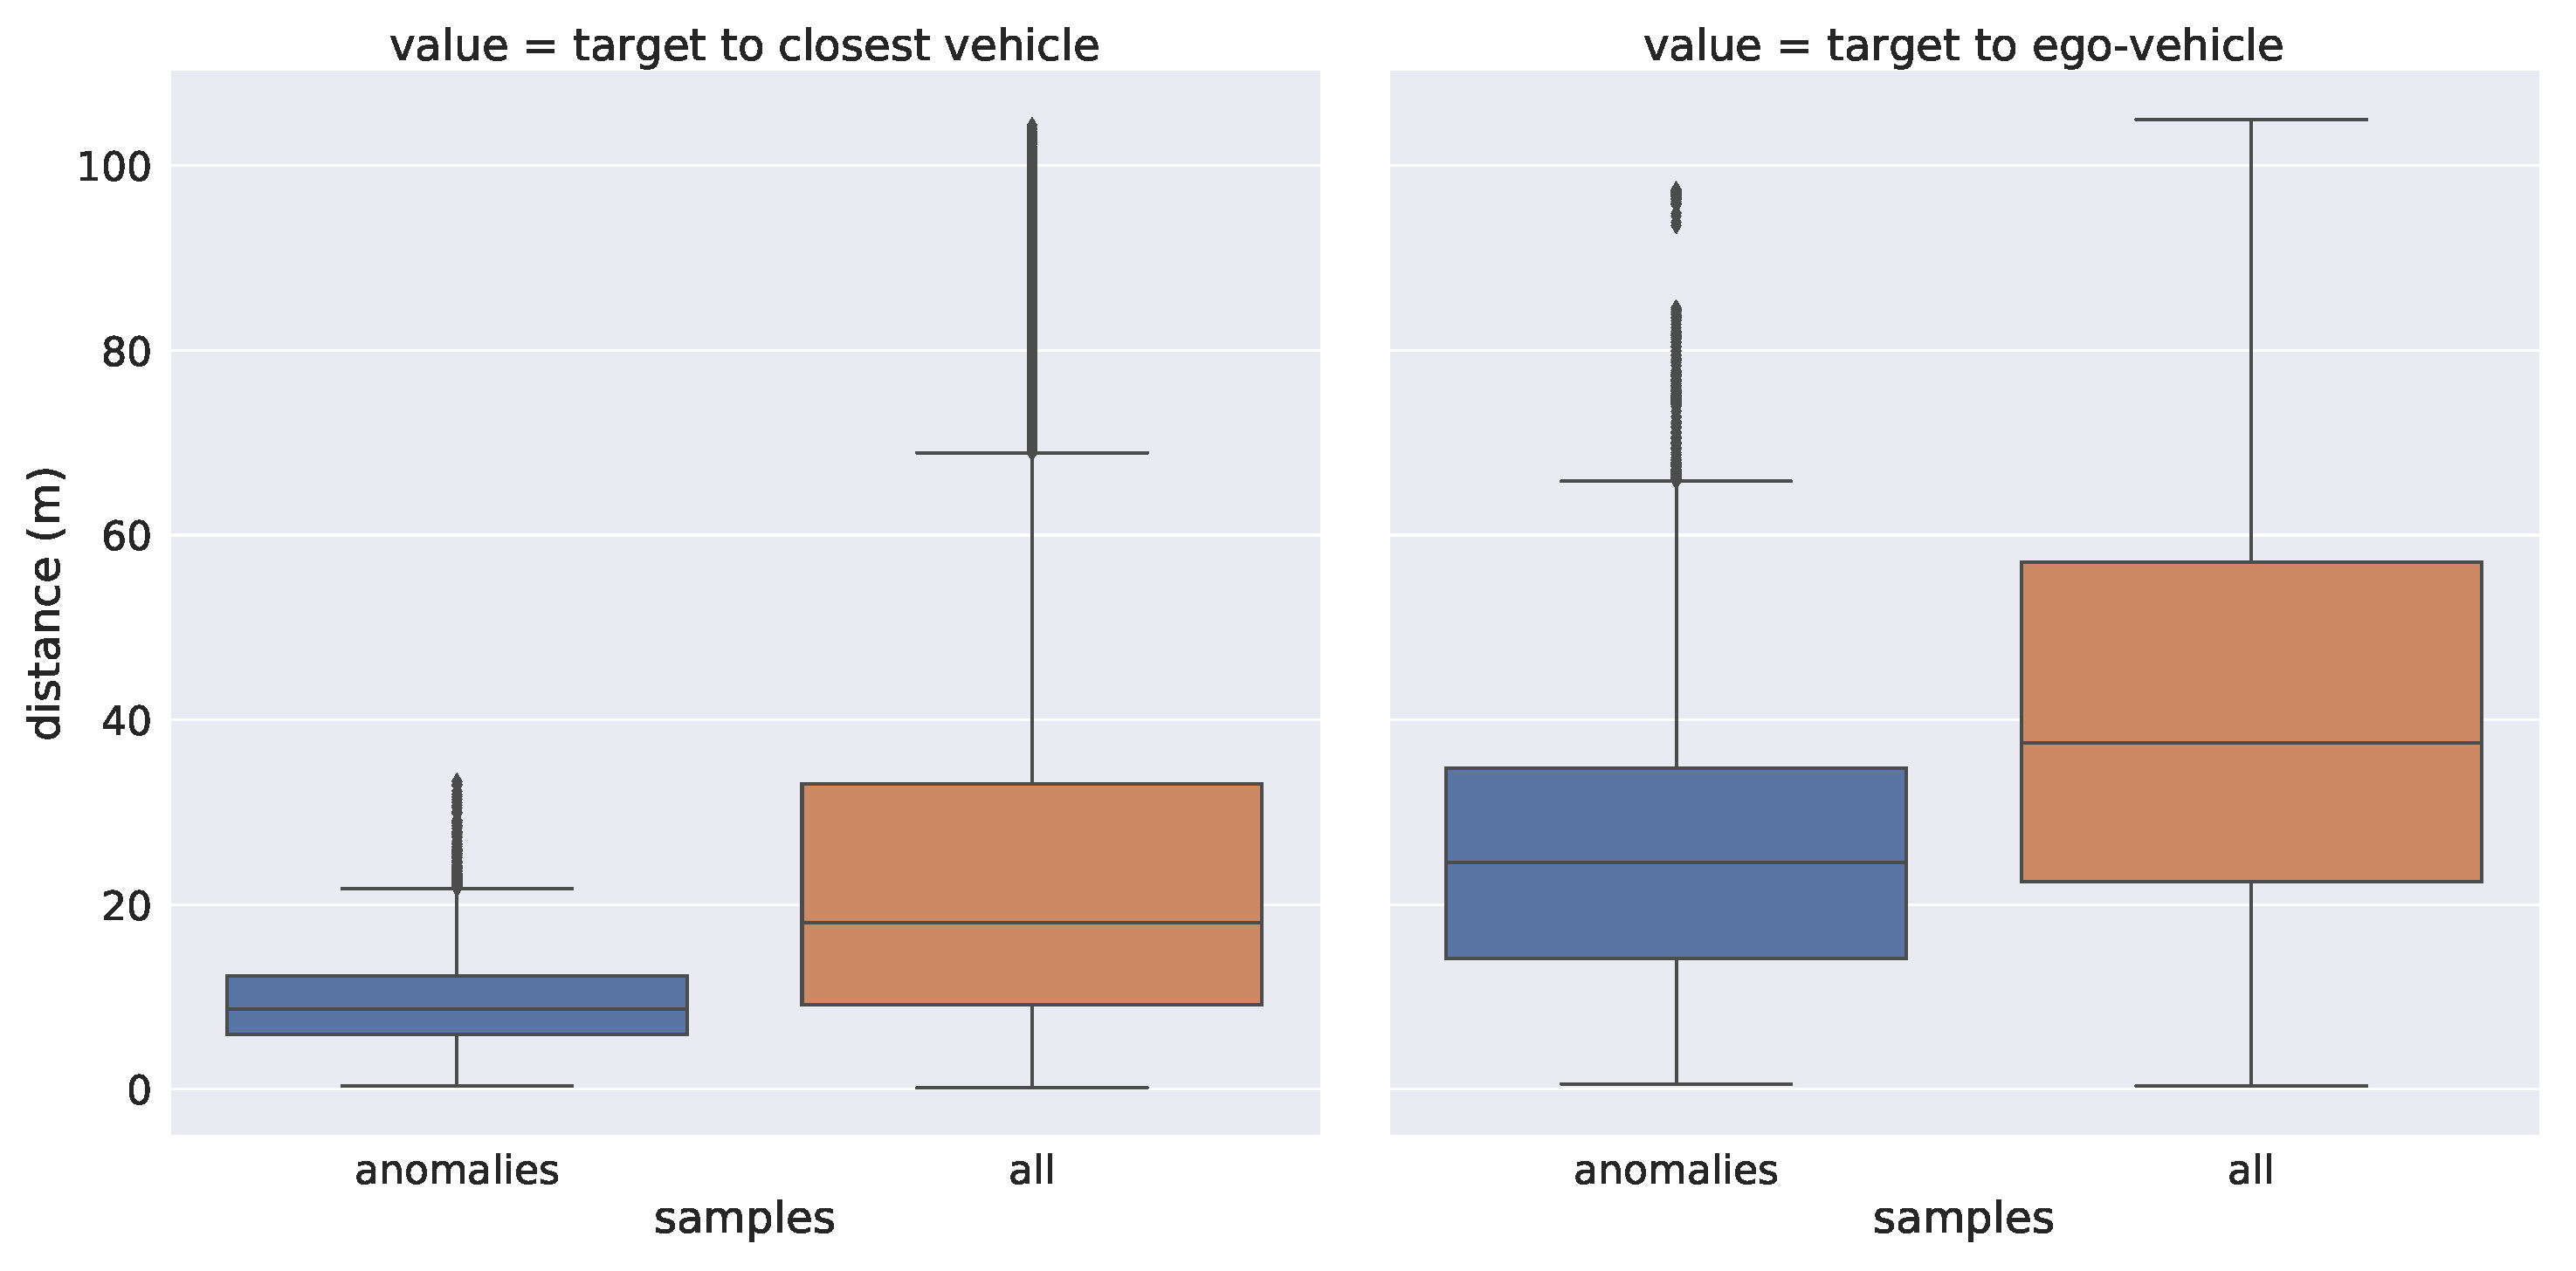
\includegraphics[width=0.5\linewidth]{imgs/anomalies_on_board_boxplots_distances.eps}
    }
    \subfloat[\label{subfig:anomalies_on_board_boxplots_other_vehicles}]{%
        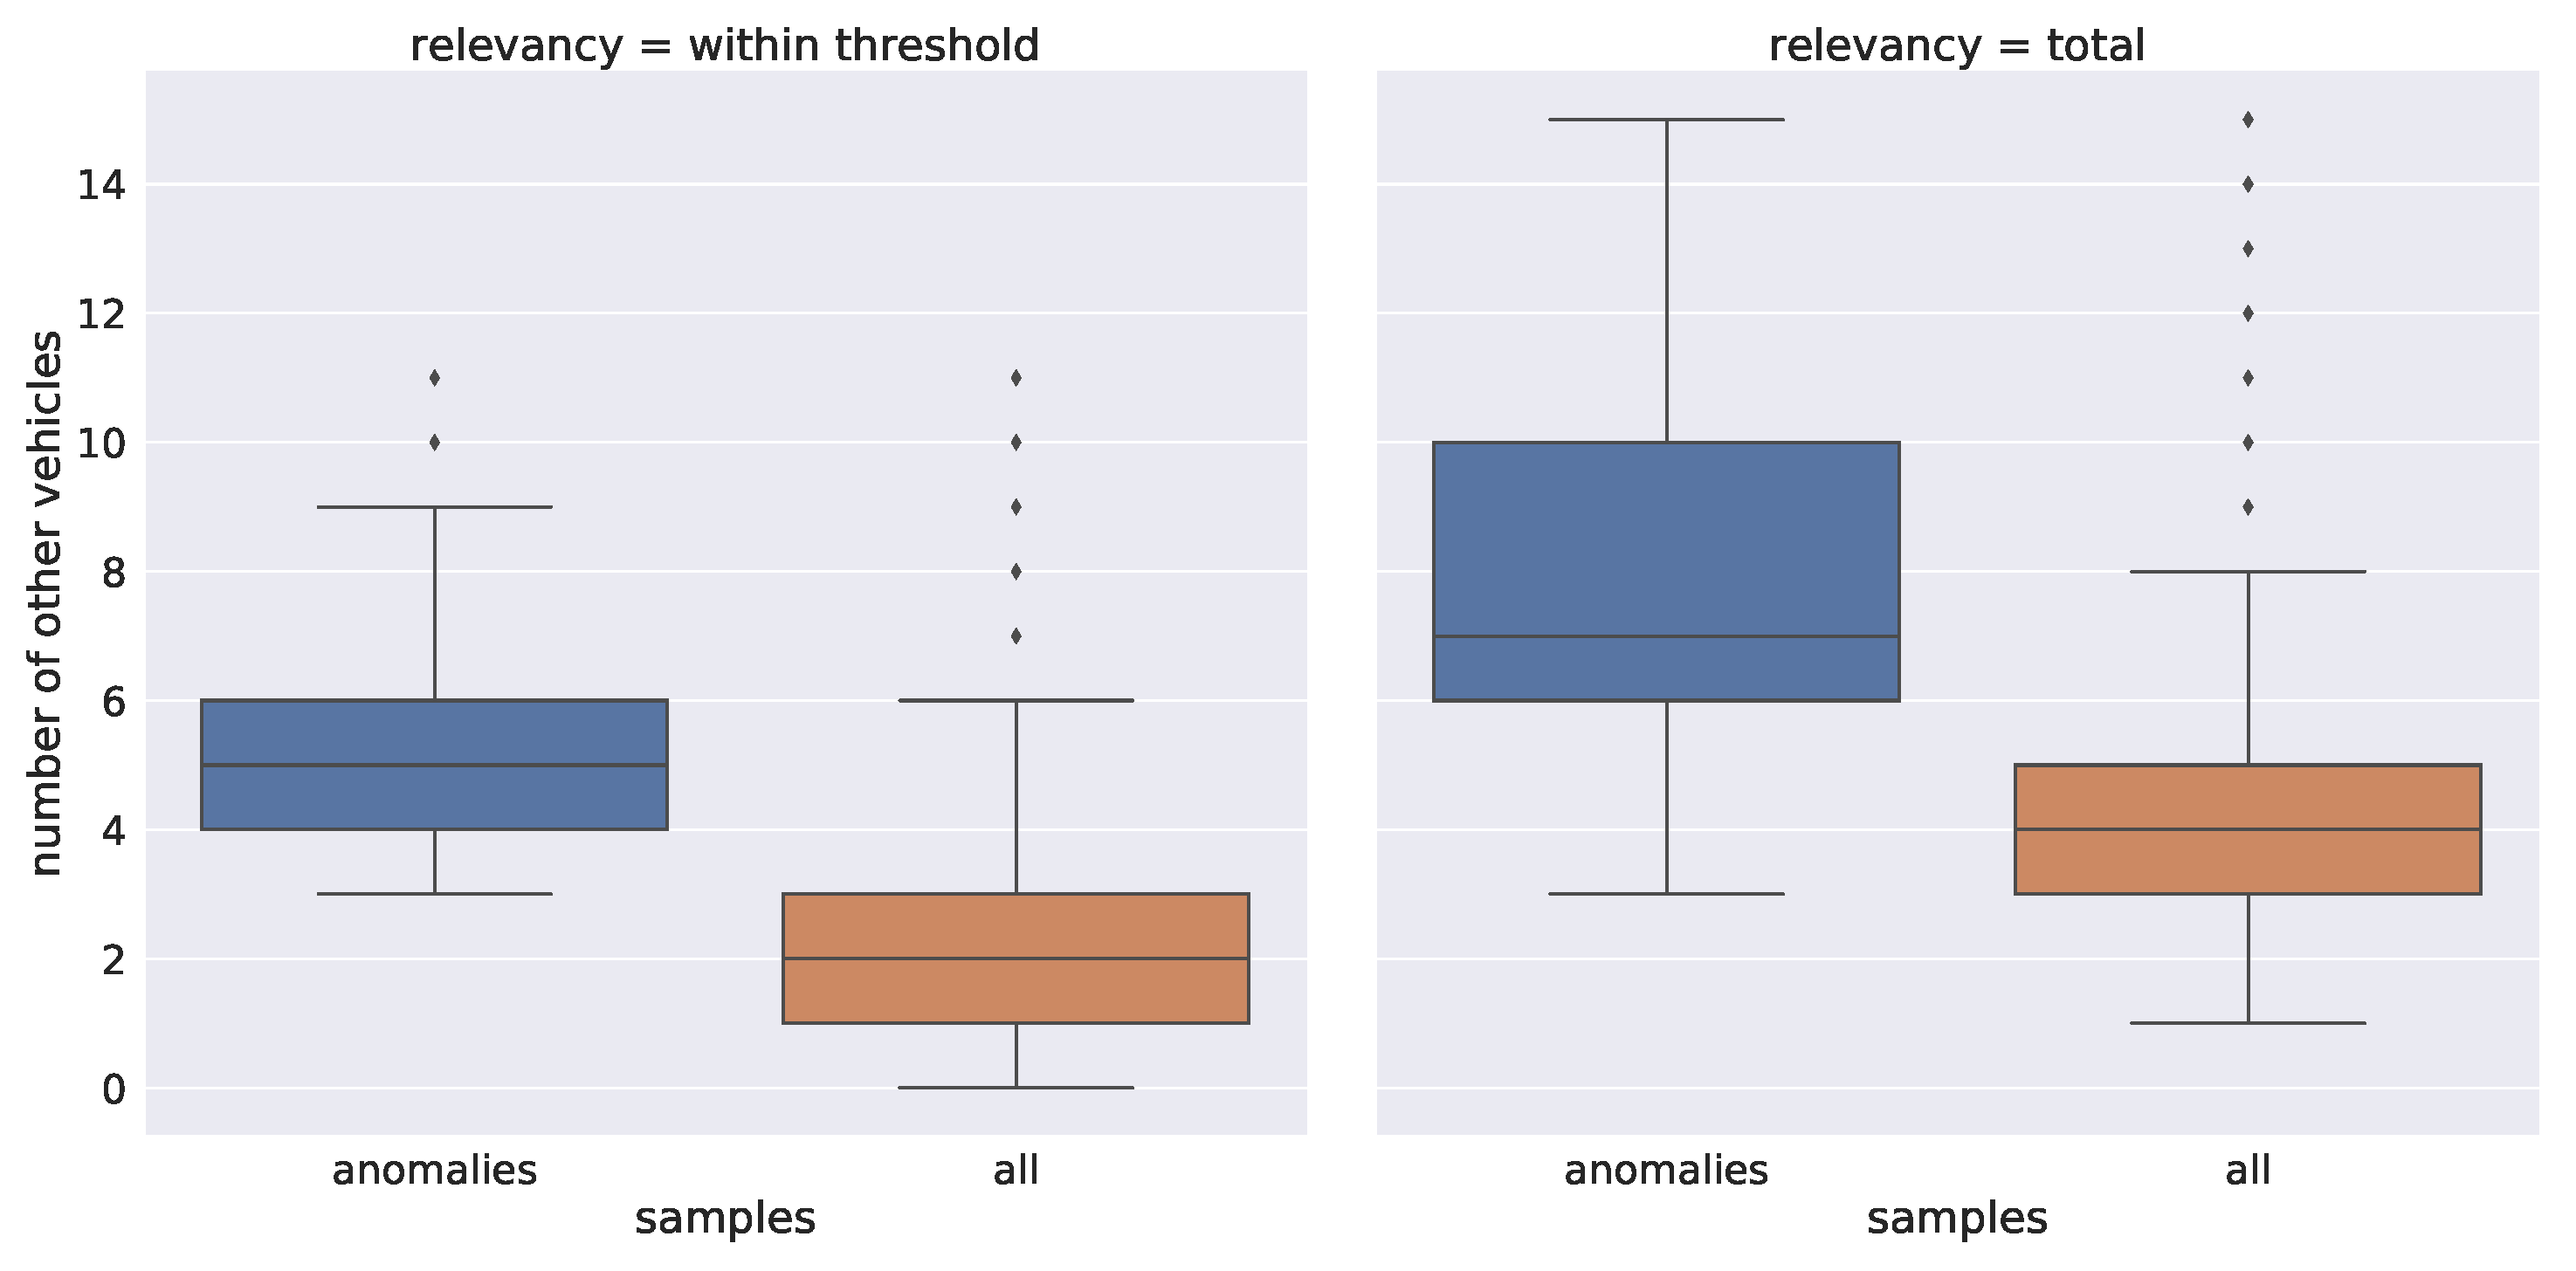
\includegraphics[width=0.5\linewidth]{imgs/anomalies_on_board_boxplots_other_vehicles.eps}
    }\\
    \subfloat[\label{subfig:anomalies_on_board_histograms_distances}]{%
        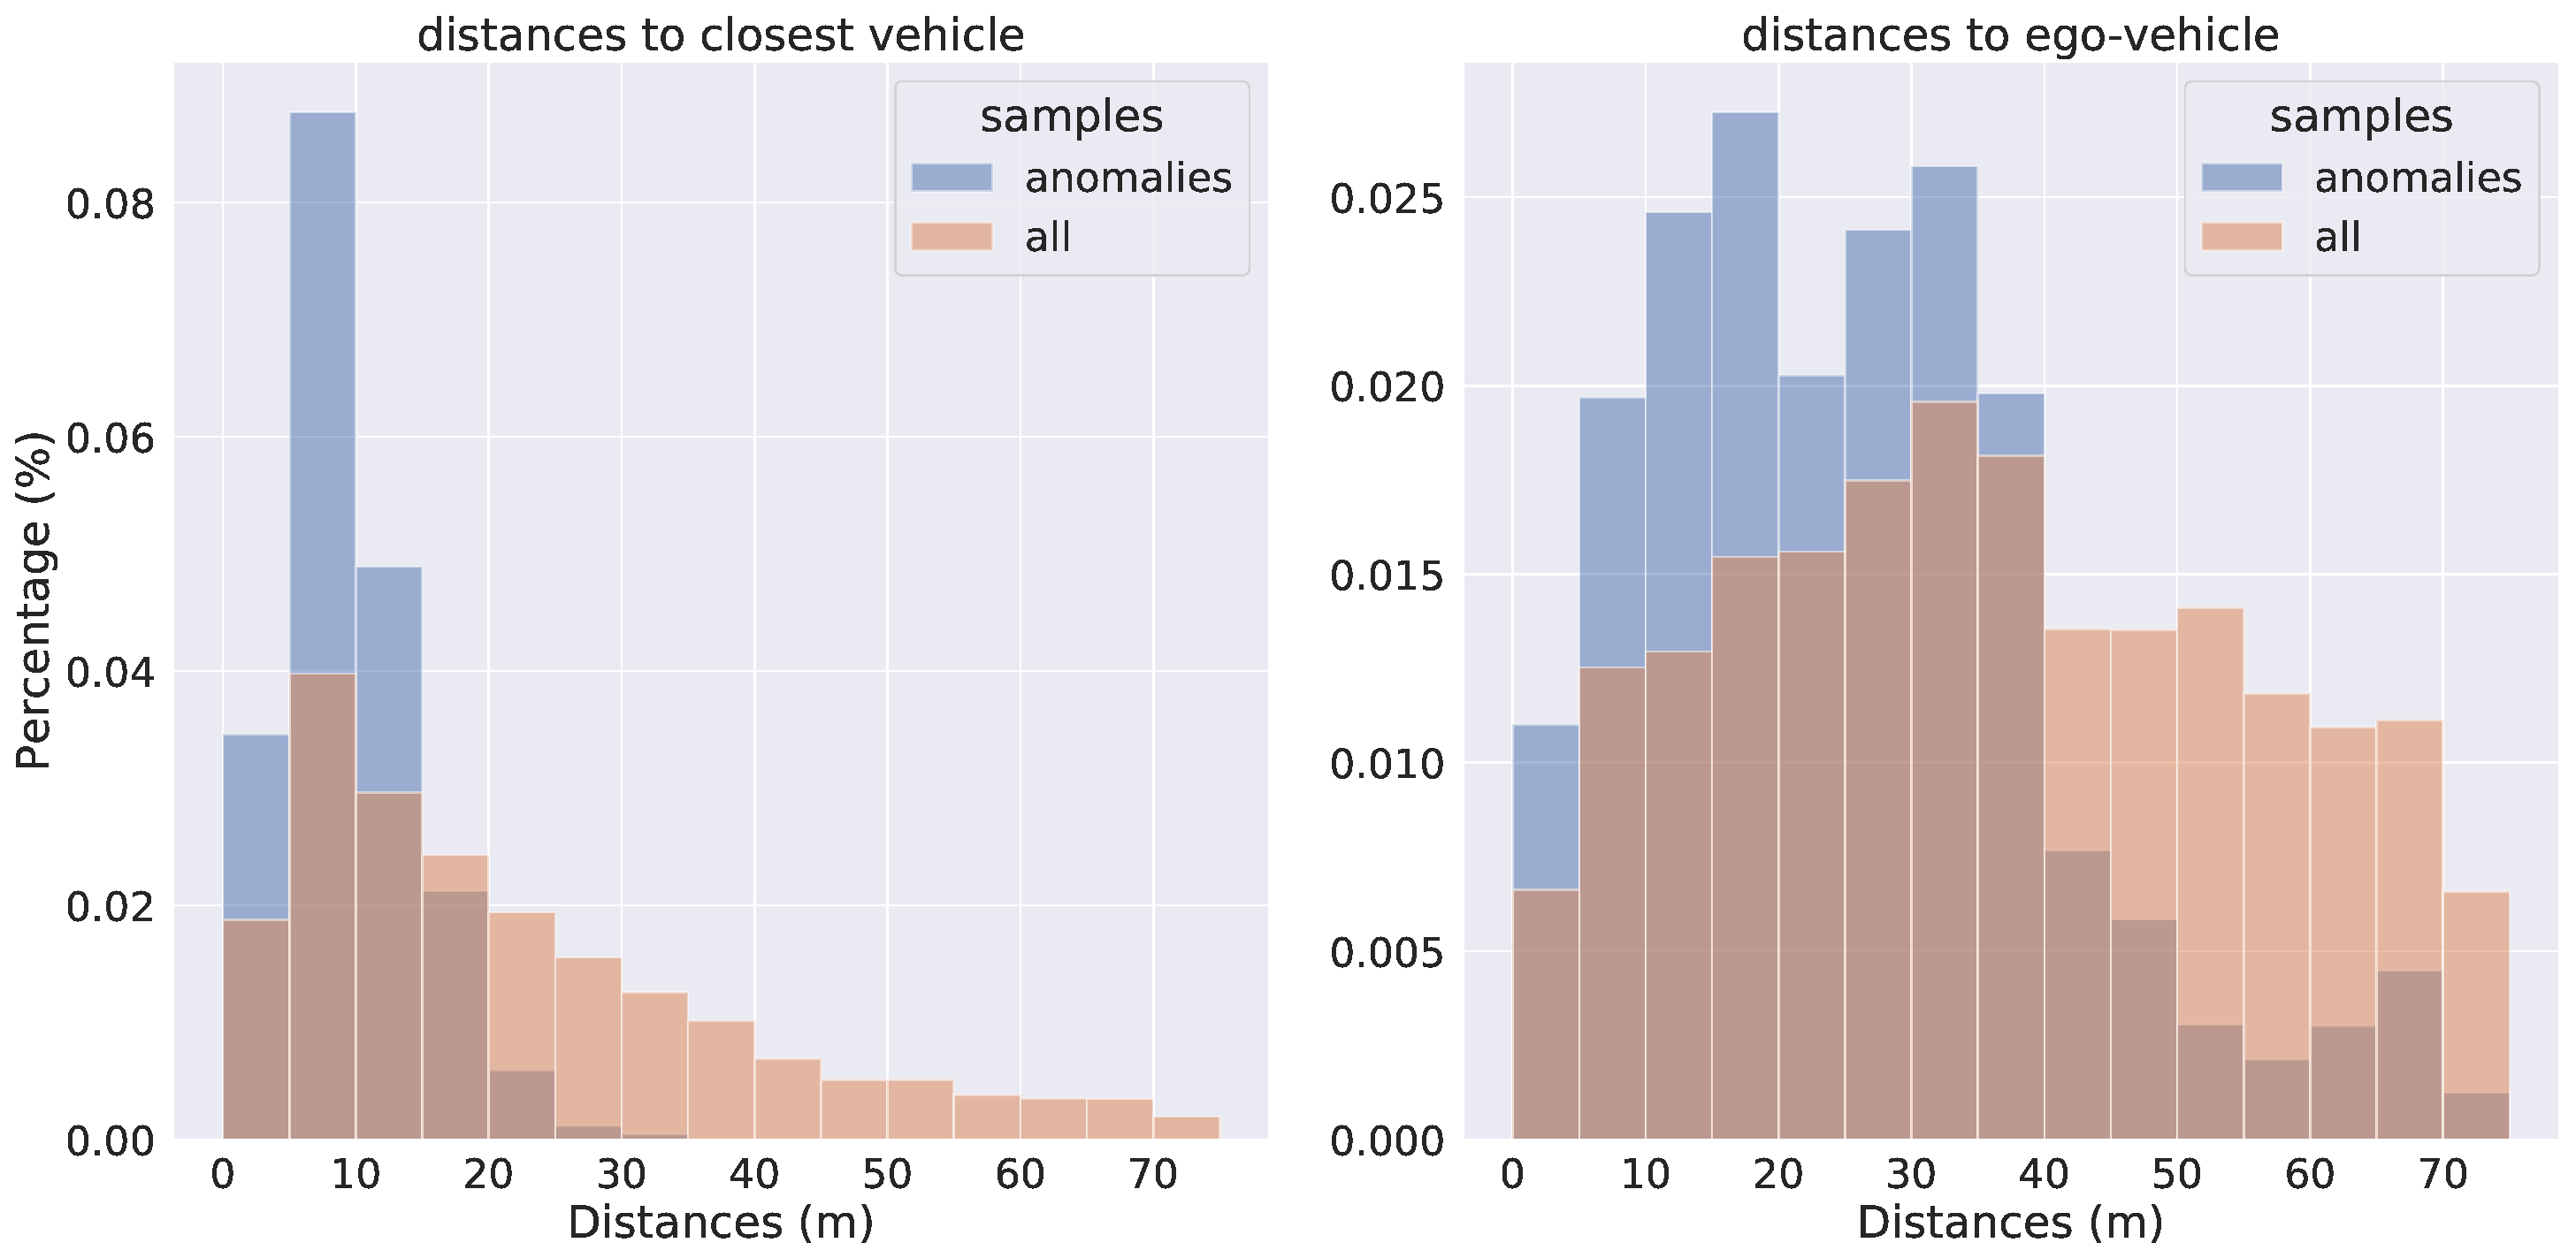
\includegraphics[width=0.5\linewidth]{imgs/anomalies_on_board_histograms_distances.eps}
    }
    \subfloat[\label{subfig:anomalies_on_board_histograms_other_vehicles}]{%
        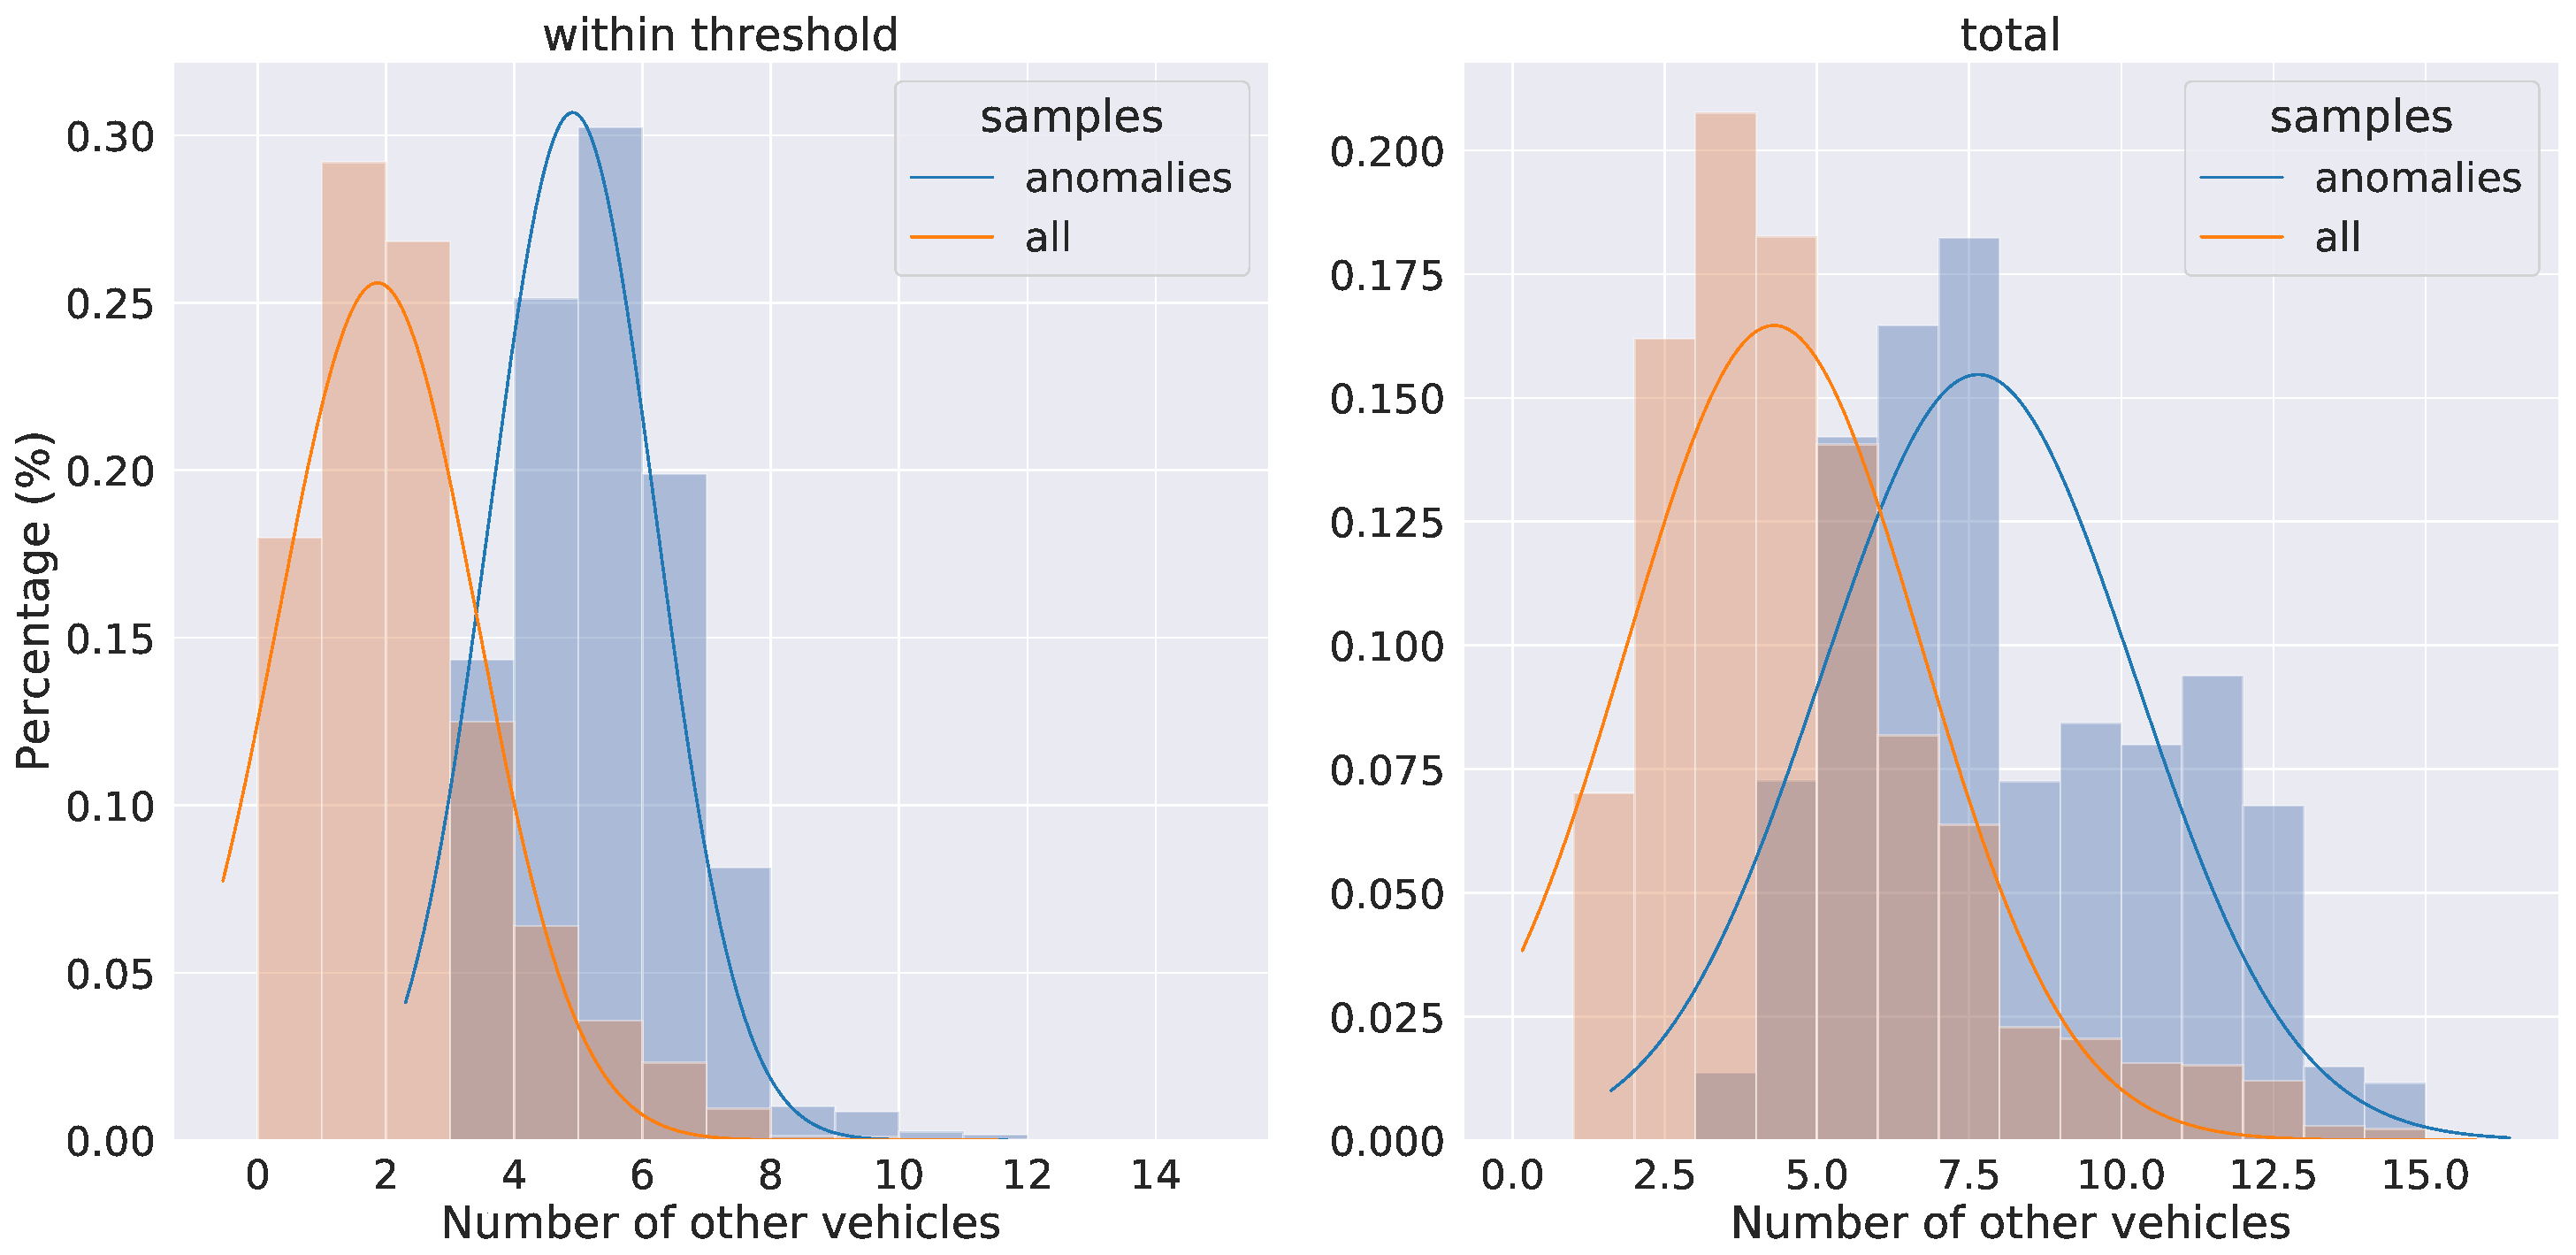
\includegraphics[width=0.5\linewidth]{imgs/anomalies_on_board_histograms_other_vehicles.eps}
    }
    \caption{Visualization of the results of the autoencoder neural network used for unsupervised anomaly detection on the \emph{On-board} data set.
        The figures show the distribution of certain characteristic values, namely distances between the target and other vehicles (Fig.~\protect\subref{subfig:anomalies_on_board_boxplots_distances} and~\protect\subref{subfig:anomalies_on_board_histograms_distances}) as well as the number of other vehicles (Fig.~\protect\subref{subfig:anomalies_on_board_boxplots_other_vehicles} and~\protect\subref{subfig:anomalies_on_board_histograms_other_vehicles}), for situations classified as anomalies and for the complete data set.
        The upper row shows box plots to visualize the difference between anomalies and the complete data set, whereas the lower row shows histograms for a more in-depth visualization of the metrics' distribution.
}
    \label{fig:anomaly_on_board}
\end{figure}

In this section, we analyze and evaluate the results of the performance of the anomaly detection network introduced in section~\ref{subsec:excursion_on_unsupervised_anomaly_detection}.
We train a fully-connected autoencoder neural network with \num{4} hidden layers consisting of \num{64}, \num{32}, \num{32} and \num{64} neurons in unsupervised fashion to generate replicates of the original vectors used as input to the network.
We use the reconstruction error between the original vectors and the replicates generated by the neural network as anomaly score and calculate a threshold for the error to detect outliers based on the percentage of anomalies we expect in the data set.
For this evaluation, we use \SI{10}{\percent} for the amount of expected outliers within the data set and trained the network for \num{100} epochs on the vectors encoding the current scene using the convolutive power representation as described in section~\ref{ssubsec:convolutive_power_representation}.

Since the data we are using to train the network is unlabeled, i.e., we do not have any information available which vectors belong to unusual or atypical situations, we have no way of comparing the results produced by the neural network with actual ground truth data.
Hence, our only option is to analyze the anomalies detected by our neural network with respect to certain characteristic values describing the driving situation and compare them to the values of the complete data set.
If this comparison uncovers significant differences between the anomalies detected by the neural network and the entirety of all data samples, we can at least conclude that the anomalies are reasonably different from the rest of the data set and furthermore, that there is sufficient information encoded in our vector representation to unravel them.
For this analysis, we use the same metrics already analyzed in section~\ref{ssubsec:evaluation_nef} to characterize crowded and potentially dangerous driving situations, namely the distance between the target and the ego-vehicle, the distance between the target and the closest other vehicle and the number of other vehicles present in the scene.
Figure~\ref{fig:anomaly_on_board} visualizes the distribution of these metrics on the set of anomalies produced by the neural network and on all data samples in the \emph{On-board} data set.
Figure~\ref{subfig:anomalies_on_board_boxplots_distances} shows box plots of the distances between the target and the closest other vehicle (left plot in Fig.~\ref{subfig:anomalies_on_board_boxplots_distances}) as well the target and the closest other vehicle (right plot in Fig.~\ref{subfig:anomalies_on_board_boxplots_distances}) while Fig.~\ref{subfig:anomalies_on_board_histograms_distances} shows the same data, but illustrated as histograms.
Figure~\ref{subfig:anomalies_on_board_boxplots_other_vehicles} and~\ref{subfig:anomalies_on_board_histograms_other_vehicles} visualize a similar evaluation for the number of other vehicles within a certain distance (left plots), namely \SI{40}{\meter}, and all other vehicles in the scene (right plots).

\begin{figure}[t]
    \centering
    \resizebox{.9\textwidth}{!}{%
        \subfloat[\label{subfig:anomalies_ngsim_boxplot_distance}]{%
            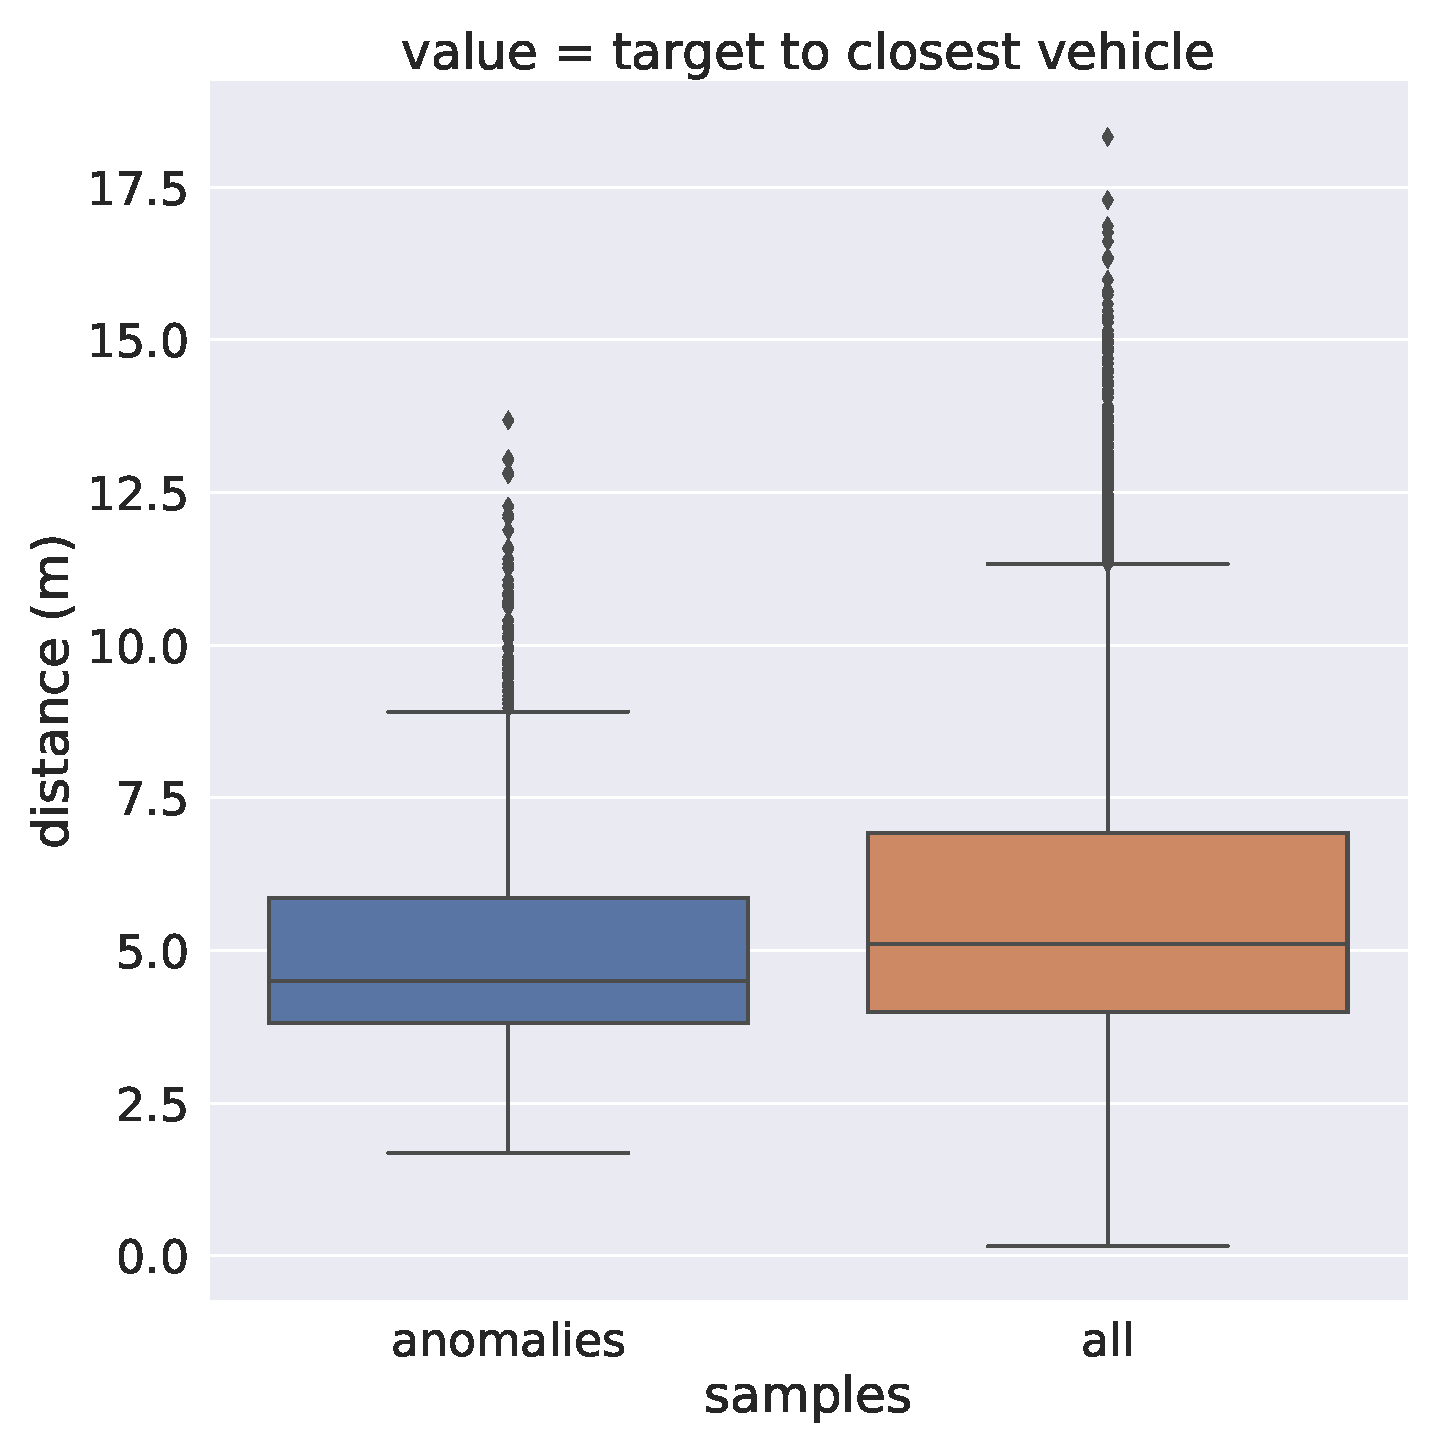
\includegraphics[height=3cm]{imgs/anomalies_ngsim_boxplot_distance.eps}
        }
        \subfloat[\label{subfig:anomalies_ngsim_histogram_distance}]{%
            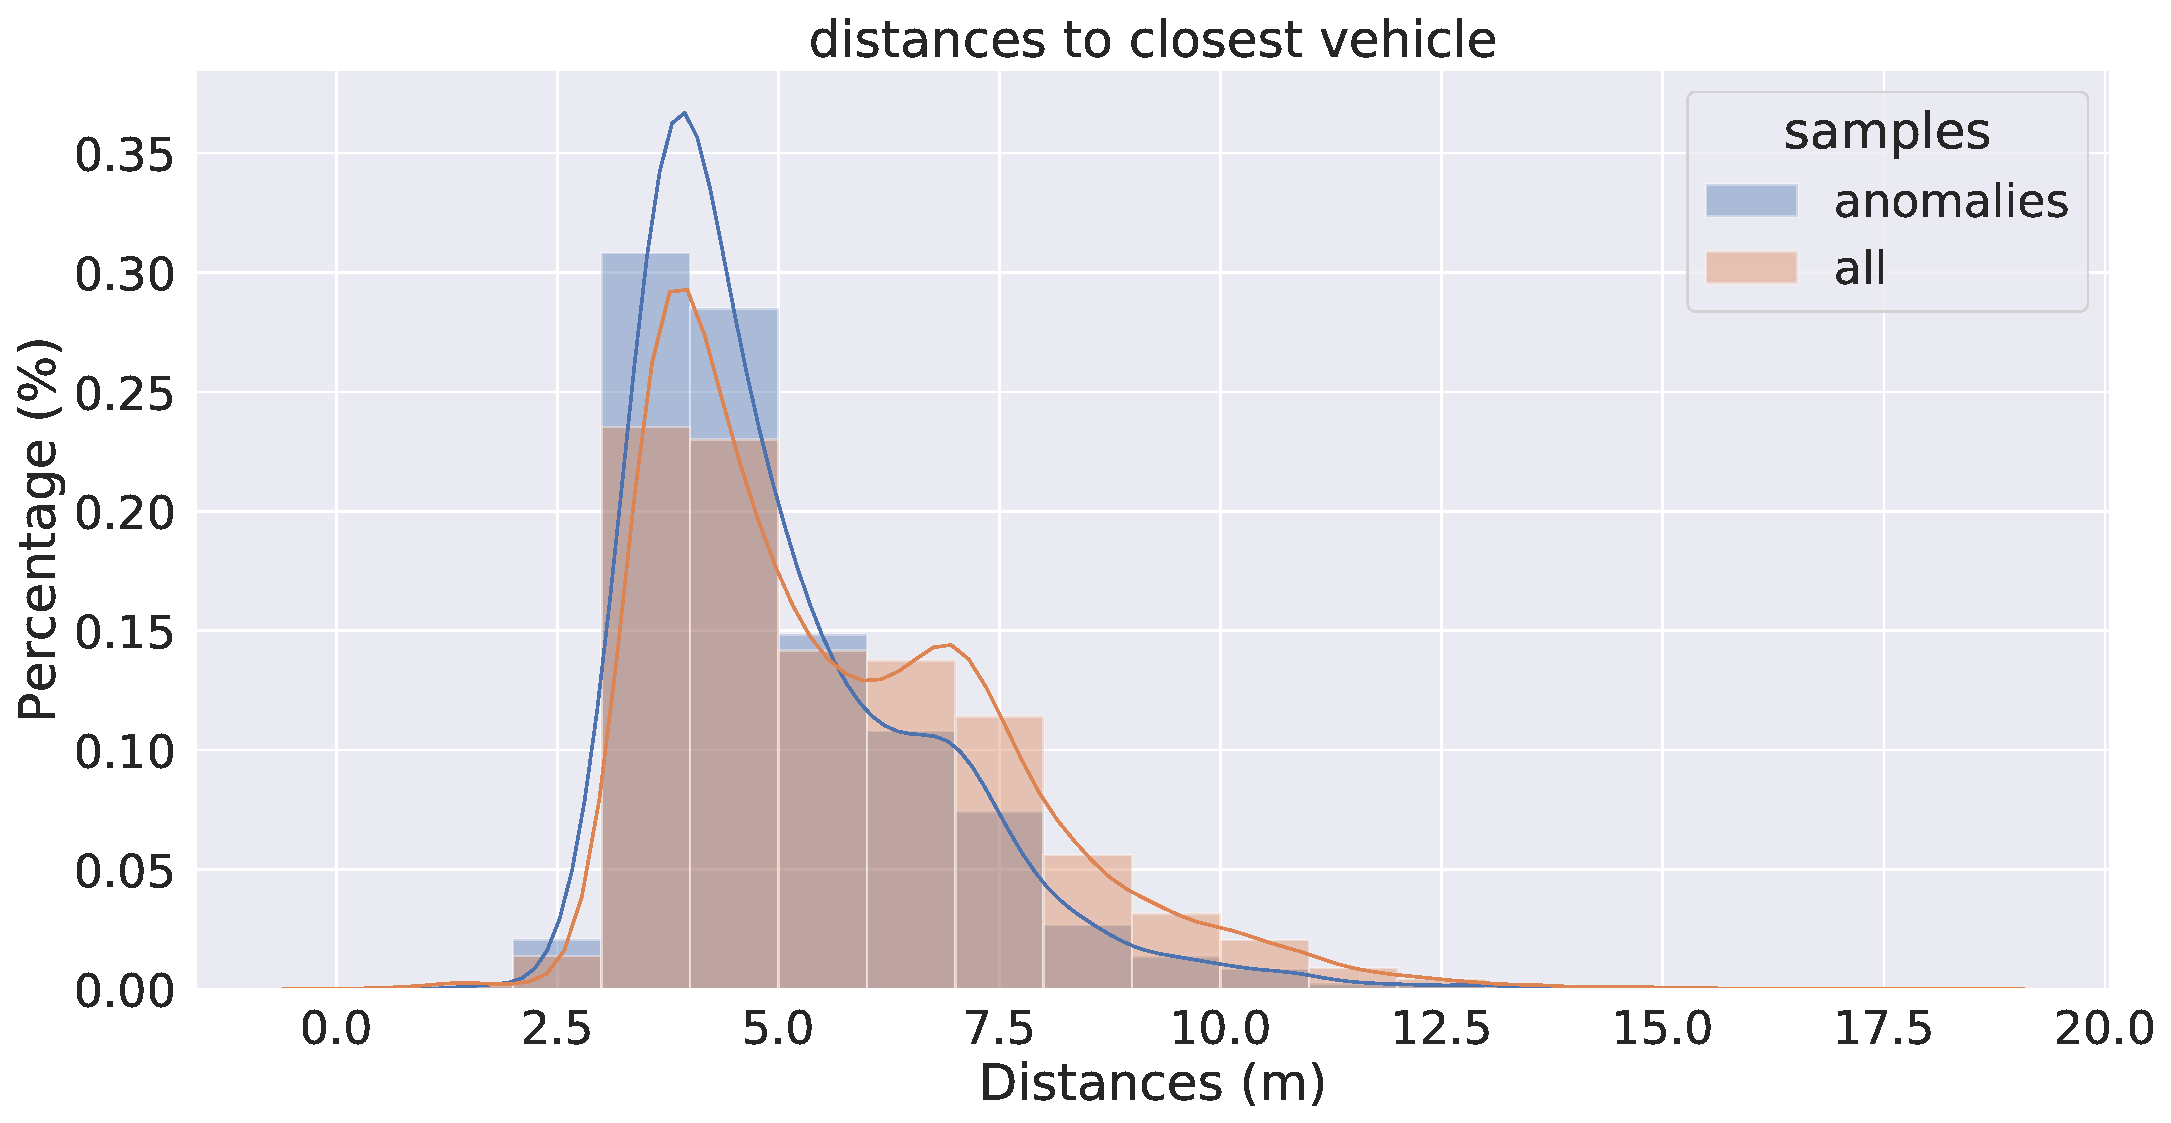
\includegraphics[height=3cm]{imgs/anomalies_ngsim_histogram_distance.eps}
        }
    }\\
    \resizebox{.9\textwidth}{!}{%
        \subfloat[\label{subfig:anomalies_ngsim_boxplot_other_vehicles}]{%
            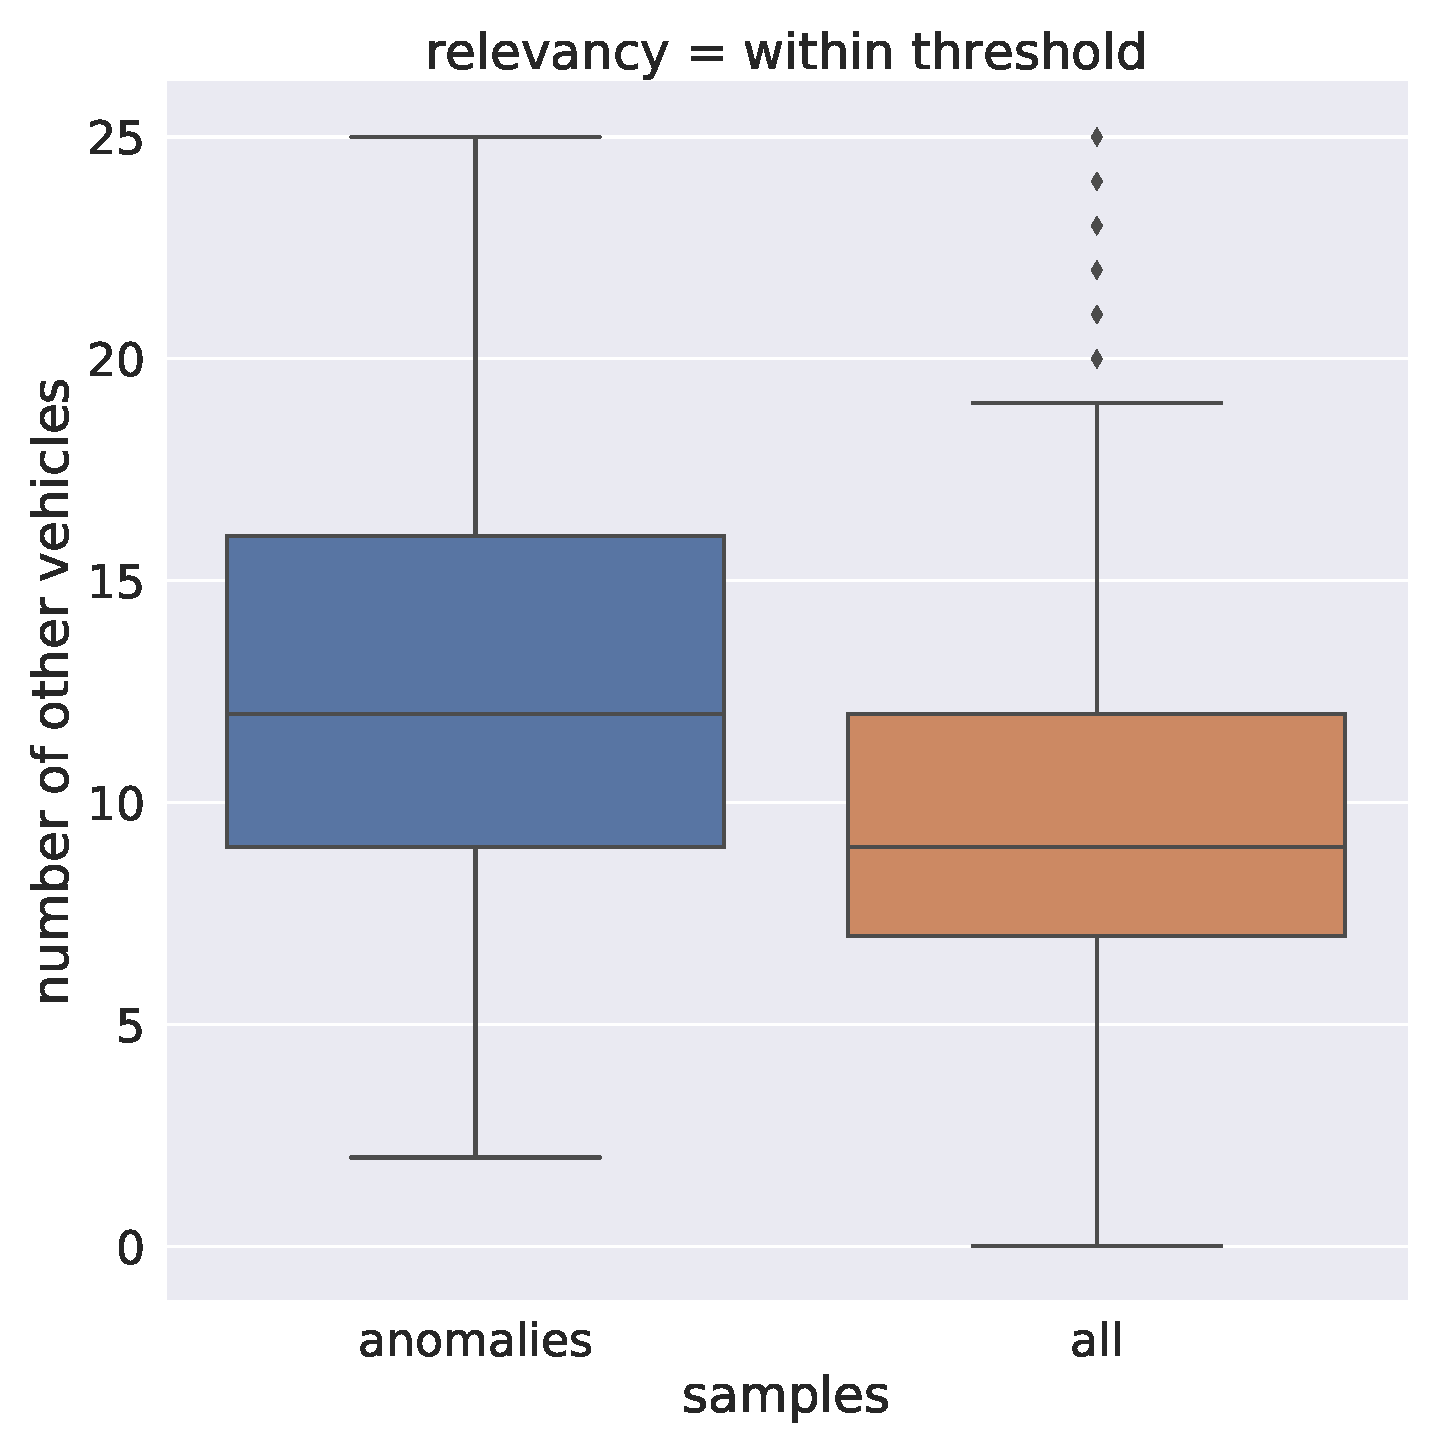
\includegraphics[height=3cm]{imgs/anomalies_ngsim_boxplot_other_vehicles.eps}
        }
        \subfloat[\label{subfig:anomalies_ngsim_histogram_other_vehicles}]{%
            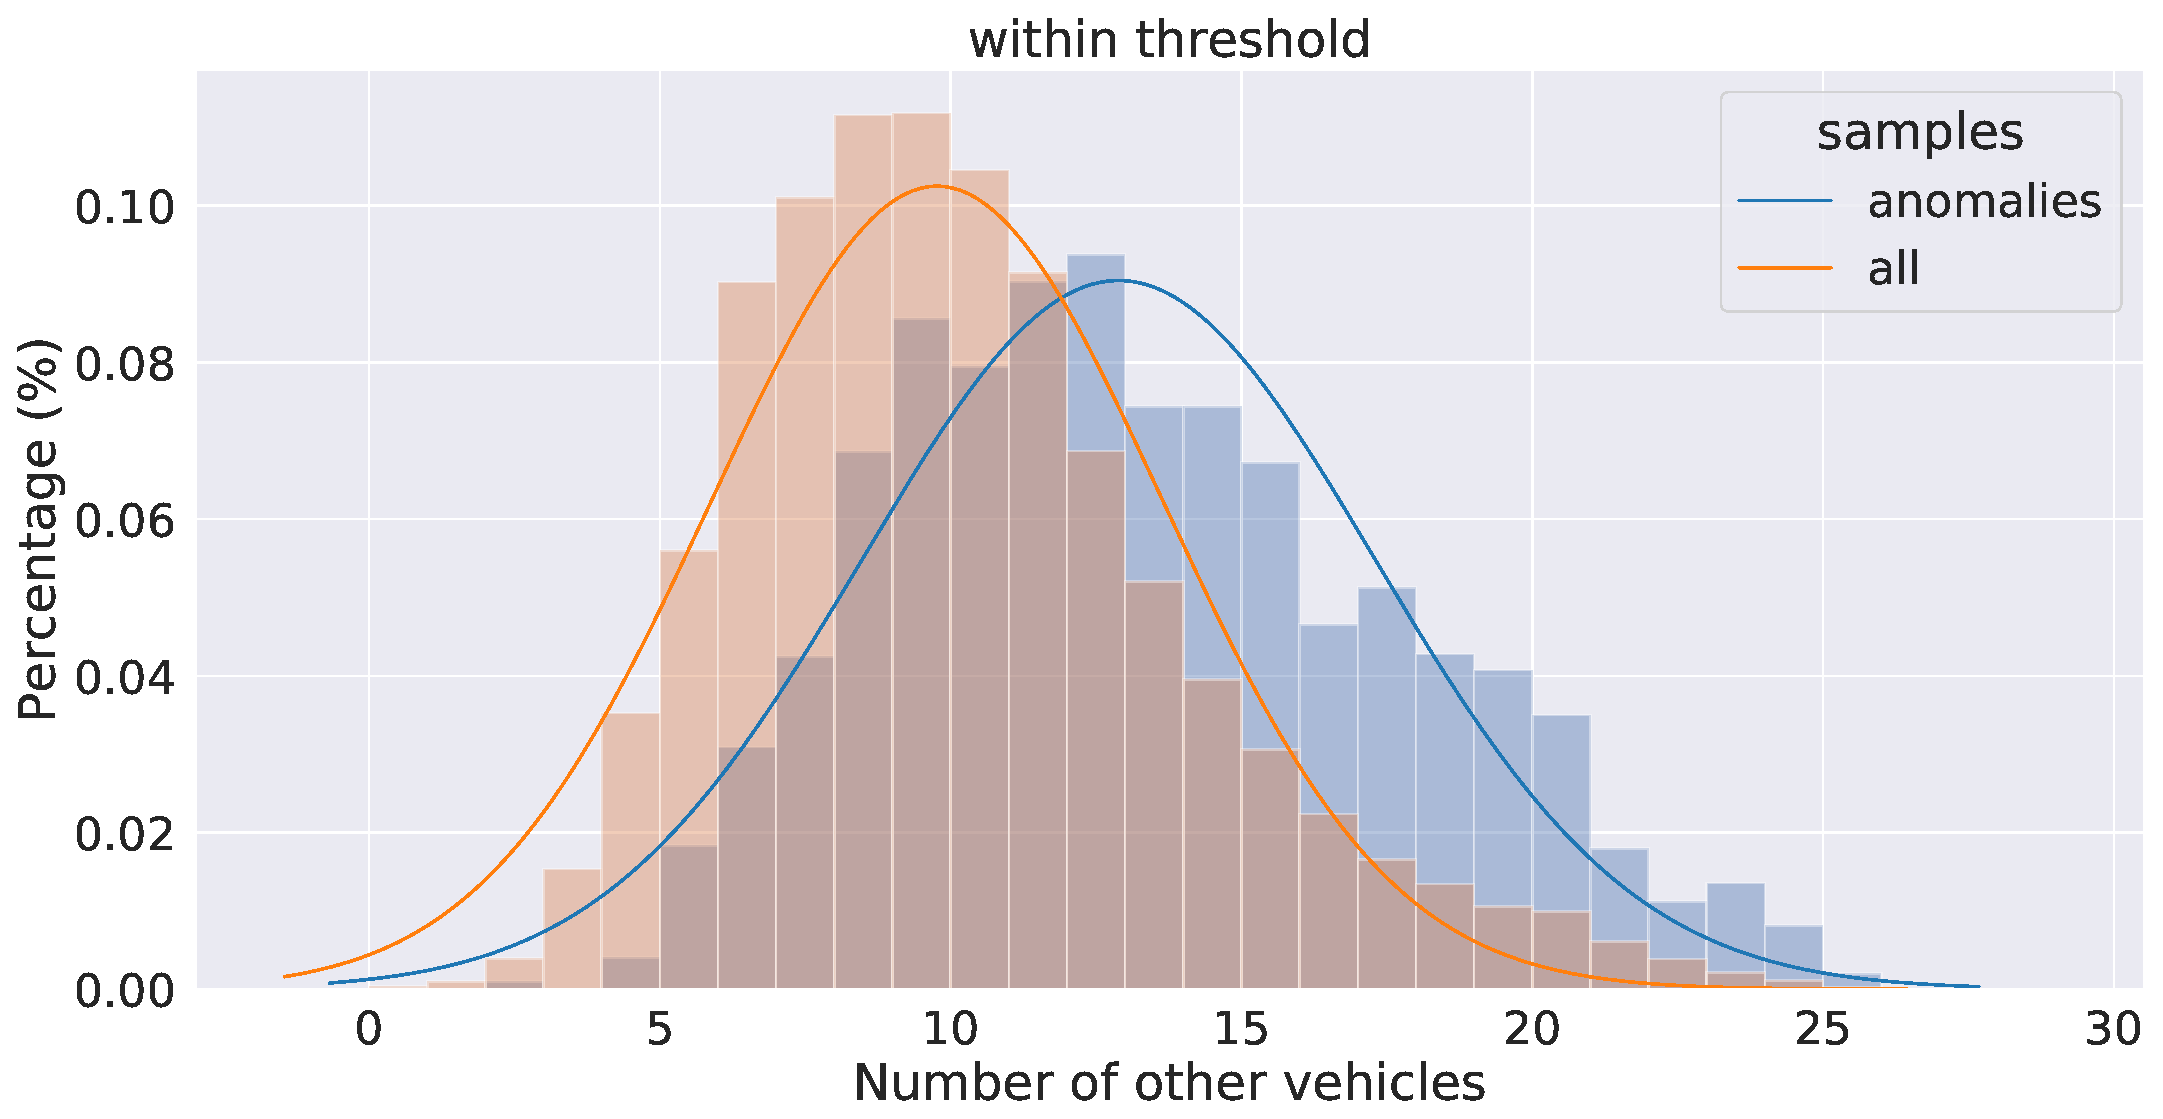
\includegraphics[height=3cm]{imgs/anomalies_ngsim_histogram_other_vehicles.eps}
        }
    }
    \caption{Visualization of the results of the autoencoder neural network used for unsupervised anomaly detection on the \emph{\ac{NGSIM}} data set.
        The figures show the distribution of distances between the target and other vehicles (Fig.~\protect\subref{subfig:anomalies_ngsim_boxplot_distance} and~\protect\subref{subfig:anomalies_ngsim_histogram_other_vehicles}) as well as the number of other vehicles (Fig.~\protect\subref{subfig:anomalies_ngsim_boxplot_other_vehicles} and~\protect\subref{subfig:anomalies_ngsim_histogram_other_vehicles}), for situations classified as anomalies and for the complete data set.
    The left figures (Fig.~\protect\subref{subfig:anomalies_ngsim_boxplot_distance} and~\protect\subref{subfig:anomalies_ngsim_boxplot_other_vehicles}) show box plots to visualize the difference between anomalies and the complete data set, whereas the right figures (Fig.~\protect\subref{subfig:anomalies_ngsim_histogram_distance} and~\protect\subref{subfig:anomalies_ngsim_histogram_other_vehicles}) show histograms for a more in-depth visualization of the metrics' distribution.}
    \label{fig:anomaly_ngsim}
\end{figure}

We observe a clear difference for both, the evaluation of the distances and the number of other vehicles, between the anomalies detected by our neural network and the complete set of data samples.
Focusing on the distance information, the number of instances with smaller distances between the ego-vehicle or the closest other vehicle and the target is significantly higher for the anomalies than for the complete data set.
While the mean distance between the target and closest other vehicle is slightly below \SI{20}{\meter} for the complete data set, the mean distance for the anomalies is \SI{10}{\meter} (cf.\ Fig.~\ref{subfig:anomalies_on_board_boxplots_distances}) with clear concentration below \SIrange{0}{15}{\meter} (cf.\ Fig.~\ref{subfig:anomalies_on_board_histograms_distances}).
We observe a similar distribution for the distance between the target and the ego-vehicle, where the distances are more or less equally distributed around the mean of \SI{40}{\meter} for the complete data set.
For the anomalies, we observe a concentration of the distances between the target and the ego-vehicle below \SI{40}{\meter} around the mean of \SI{25}{\meter}.
Regarding the number of other vehicles, the difference between the complete data set and the anomalies detected by our neural network is even clearer.
For the complete data set, the mean number of other vehicles within \SI{40}{\meter} to the target vehicle is \num{2}, while the total mean number of other vehicles is around \num{4}.
Both numbers are significantly higher for the anomalies with a mean number of \num{5} other vehicles within \SI{40}{\meter} and a mean of \num{7} other vehicles in total (cf.\ Fig.~\ref{subfig:anomalies_on_board_boxplots_other_vehicles}).
Looking at the distribution shown in the histograms in Fig.~\ref{subfig:anomalies_on_board_histograms_other_vehicles}, the picture becomes even clearer. 
There are no situations with less then \num{3} other vehicles within \SI{40}{\meter} to the target vehicle in the set of anomalies, whereas in this same range fall the majority of samples of the complete data set.
We observe a similar distribution for the total number of other vehicles in the scene with the anomaly samples having at least \num{3} and the majority of examples having at least \num{4} other vehicles present in the scene.
In contrast, the great majority of samples from the complete data set has at most \num{7} other vehicles present and the overall distribution is somewhat inverse to that of the anomalies.

Figure~\ref{fig:anomaly_ngsim} shows a similar analysis for the \emph{\ac{NGSIM}} data set with a few systematic differences.
Since the \emph{\ac{NGSIM}} data set is recorded with external cameras observing highway traffic, there is no ego-vehicle to evaluate regarding the distance to the target vehicle.
Hence, we only analyze the distance between the target vehicle and the closest other vehicle (see Fig.~\ref{subfig:anomalies_ngsim_boxplot_distance} and~\ref{subfig:anomalies_ngsim_histogram_distance}).
Furthermore, since the external cameras record highway traffic on \num{6} lanes on a segment of \SI{640}{\meter} length for the \emph{\ac{NGSIM}} data set, we needed to reduce the number of vehicles to be included in our vector representation to the ones most relevant for the prediction task.
Therefore, we focus on vehicles within a distance of \SI{40}{\meter} on lanes adjacent to the target vehicle's lane for the analysis of our anomaly detection network here as well (see Fig.~\ref{subfig:anomalies_ngsim_boxplot_other_vehicles} and~\ref{subfig:anomalies_ngsim_histogram_other_vehicles}).
While the differences between anomalies and the complete data set regarding the distance between the target and the closest other vehicle is not as significant for the \emph{\ac{NGSIM}} data set in comparison to the \emph{On-board} data set, we still observe a similar tendency for the anomalies to capture situations with smaller distances between the target and the closest other vehicle.
For the number of other vehicles however, we also observe that the samples detected as anomalies by our autoencoder network tend to have more vehicles in the target vehicle's surroundings present than for all the samples within the \emph{\ac{NGSIM}} data set.

In conclusion, our autoencoder neural network is able to detect a subset of anomalies consistently for both, the \emph{On-board} and \emph{\ac{NGSIM}} data set, which show sufficiently significant differences to the complete data set regarding certain metrics.
The results indicate, that the anomalies detected by the network have a tendency towards crowded situations with rather small distances between the target vehicle and the other vehicles in its surroundings.
Since these are the kind of situations, where our prediction models based on the \ac{SPA}-based convolutive power encoding tend to perform better than the other reference models, these results offer interesting directions for future research.
For instance, we could combine the anomaly detection network based on our vector representation presented in this section with the behavior prediction networks to decide whether the current driving situation is potentially hazardous and needs more accurate predictions than less crowded or dangerous situations. 
We have already seen in section~\ref{subsec:evaluation_of_the_lstm_based_prediction_models}, that the \ac{LSTM} models employing the convolutive power representation (\ac{LSTM} \ac{SPA} \num{1} and \num{3}) outperform the other models in such situations particularly in lateral direction. 
Furthermore, one could also imagine to let the outlier detection network guide the training process of the behavior prediction networks.
That is, we could train prediction models particularly on lane changes, the outliers and a similar amount of \enquote{normal} samples to create a more balanced training data set.
We have already seen that the networks using semantic vectors benefit from a more focused and specific training data set, since the models trained particularly on lane changes improved especially in lane change situations compared to network variants trained on all samples.
Finally, we could also investigate other anomaly detection algorithms in addition to the autoencoder models shown here to get a better idea what sort of data samples are actually  outliers by evaluating how different models classify anomalies differently.

\section{Summary}%
\label{sec:summary_behavior_prediction}

In this chapter, we showed a novel approach to encapsulate spatial information of multiple objects in a sequence of semantic pointers of fixed vector length.
We used a \ac{LSTM} sequence to sequence model as well as a simple feed-forward \acl{SNN} to predict future vehicle positions from this representation.
For each of those models, we implemented at least one reference model using other encoding schemes to compare their performance to.
Furthermore, we compared all our models to a simple linear predictor based on a constant velocity assumption.
We evaluated our models on two different data sets, one recorded with on-board sensors from a driving vehicle and one publicly available trajectory data set recorded with an external camera observing a highway segment and conducted a thorough analysis.

For the trained neural networks, simple feed-forward \ac{NEF} models and more sophisticated \ac{LSTM} models alike, we observe that most improvements over the linear model are achieved in $y$-direction.
That makes sense as linear prediction is unable to account for lane-changes or driving curves, which are mainly characterized by non-linear changes in $y$-direction.
We found that the \ac{LSTM} models based on our \ac{SPA}-power representation achieve promising results on both data sets.
However, for the \emph{On-board} data set, this encoding scheme achieves its best result in crowded and potentially dangerous driving situations, without clearly outperforming the other approaches on the whole data set (see section~\ref{subsec:evaluation_of_the_lstm_based_prediction_models} and Fig.~\ref{fig:rmse_on_board_all}).
Given these finding, we investigated situations, where the \ac{SPA}-power representation does outperform all other approaches in $y$-direction and thereby came up with metrics characterizing such crowded situations (see Fig. \ref{fig:histograms_on_board}).
This result did not hold that clearly on the \emph{\ac{NGSIM}} data set $D_2$, since the \ac{LSTM} models achieve an almost identical performance in $y$-direction on this data set.
On the other hand, employing an unsupervised learning method for anomaly detection yielded a significantly higher amount of such crowded situations within the samples classified as anomalies compared to the normal samples.
Additionally, we found that when training the \ac{LSTM} models only on data samples containing a lane change performed by the target vehicle, that the model employing the \ac{SPA}-power representation clearly outperforms all other approaches in $y$-direction when evaluated on the samples containing a lane change.
These results suggest that training the whole system on a more balanced data set containing equally many lane change and straight driving samples could improve overall model performance.

Another interesting result of our experiments is the fact that the simple, feed-forward \ac{NEF} networks show results comparable to the more sophisticated \ac{LSTM} models.
For those simple models, the \ac{SPA}-power representation shows promising results comparable to the \ac{NEF} model using numerical input on the \emph{On-board} data set and clearly outperforming it on the \emph{\ac{NGSIM}} data set (Fig. \ref{fig:rmse_nef_nets}).
Although the \ac{NEF} models do not clearly outperform the \ac{LSTM} models (which would be surprising), it is quite remarkable that they achieve results comparable to the more sophisticated models with a simpler network architecture, training procedure and, partly, less information.
These results make those simple models using our proposed vector-representation as well as a numerical encoding scheme (possibly in combination with an online learning system like the one proposed in chapter~\ref{chap:mix_online_learning}) potential candidates to be deployed on dedicated neuromorphic hardware in mobile applications, as they can be efficiently implemented in a spiking neuron substrate.
This could be an interesting, power-efficient approach in future automated vehicles.

Finally, given the results that there is not one model clearly outperforming all the others in all evaluated situations, we aim to implement an online model meant to be trained at run time to weight the predictions of several models, which have been trained offline, to improve over the individual predictors.
We will introduce and evaluate such a model in the next chapter.
